%&preformat-synopsis
\RequirePackage[l2tabu,orthodox]{nag} % Раскомментировав, можно в логе получать рекомендации относительно правильного использования пакетов и предупреждения об устаревших и нерекомендуемых пакетах

% Откомментируйте, чтобы отключить генерацию закладок в pdf
% \PassOptionsToPackage{bookmarks=false}{hyperref}
\documentclass[a5paper,10pt,oneside,openany,article]{memoir} %,draft

%%%%%%%%%%%%%%%%%%%%%%%%%%%%%%%%%%%%%%%%%%%%%%%%%%%%%%%
%%%% Файл упрощённых настроек шаблона автореферата %%%%
%%%%%%%%%%%%%%%%%%%%%%%%%%%%%%%%%%%%%%%%%%%%%%%%%%%%%%%

%%% Инициализирование переменных, не трогать!  %%%
\newcounter{showperssign}
\newcounter{showsecrsign}
\newcounter{showopplead}
%%%%%%%%%%%%%%%%%%%%%%%%%%%%%%%%%%%%%%%%%%%%%%%%%%%%%%%

%%% Список публикаций %%%
\makeatletter
\@ifundefined{c@usefootcite}{
  \newcounter{usefootcite}
  \setcounter{usefootcite}{0} % 0 --- два списка литературы;
                              % 1 --- список публикаций автора + цитирование
                              %       других работ в сносках
}{}
\makeatother

\makeatletter
\@ifundefined{c@bibgrouped}{
  \newcounter{bibgrouped}
  \setcounter{bibgrouped}{0}  % 0 --- единый список работ автора;
                              % 1 --- сгруппированные работы автора
}{}
\makeatother

%%% Область упрощённого управления оформлением %%%

%% Управление зазором между подрисуночной подписью и основным текстом %%
\setlength{\belowcaptionskip}{10pt plus 20pt minus 2pt}


%% Подпись таблиц %%

% смещение строк подписи после первой
\newcommand{\tabindent}{0cm}

% тип форматирования таблицы
% plain --- название и текст в одной строке
% split --- название и текст в разных строках
\newcommand{\tabformat}{plain}

%%% настройки форматирования таблицы `plain'

% выравнивание по центру подписи, состоящей из одной строки
% true  --- выравнивать
% false --- не выравнивать
\newcommand{\tabsinglecenter}{false}

% выравнивание подписи таблиц
% justified   --- выравнивать как обычный текст
% centering   --- выравнивать по центру
% centerlast  --- выравнивать по центру только последнюю строку
% centerfirst --- выравнивать по центру только первую строку
% raggedleft  --- выравнивать по правому краю
% raggedright --- выравнивать по левому краю
\newcommand{\tabjust}{justified}

% Разделитель записи «Таблица #» и названия таблицы
\newcommand{\tablabelsep}{~\cyrdash\ }

%%% настройки форматирования таблицы `split'

% положение названия таблицы
% \centering   --- выравнивать по центру
% \raggedleft  --- выравнивать по правому краю
% \raggedright --- выравнивать по левому краю
\newcommand{\splitformatlabel}{\raggedleft}

% положение текста подписи
% \centering   --- выравнивать по центру
% \raggedleft  --- выравнивать по правому краю
% \raggedright --- выравнивать по левому краю
\newcommand{\splitformattext}{\raggedright}

%% Подпись рисунков %%
%Разделитель записи «Рисунок #» и названия рисунка
\newcommand{\figlabelsep}{~\cyrdash\ }  % (ГОСТ 2.105, 4.3.1)
                                        % "--- здесь не работает

%Демонстрация подписи диссертанта на автореферате
\setcounter{showperssign}{1}  % 0 --- не показывать;
                              % 1 --- показывать
%Демонстрация подписи учёного секретаря на автореферате
\setcounter{showsecrsign}{1}  % 0 --- не показывать;
                              % 1 --- показывать
%Демонстрация информации об оппонентах и ведущей организации на автореферате
\setcounter{showopplead}{1}   % 0 --- не показывать;
                              % 1 --- показывать

%%% Цвета гиперссылок %%%
% Latex color definitions: http://latexcolor.com/
% \definecolor{linkcolor}{rgb}{0.9,0,0}
% \definecolor{citecolor}{rgb}{0,0.6,0}
% \definecolor{urlcolor}{rgb}{0,0,1}
\definecolor{linkcolor}{rgb}{0,0,0} %black
\definecolor{citecolor}{rgb}{0,0,0} %black
\definecolor{urlcolor}{rgb}{0,0,0} %black
          % общие настройки шаблона
%%% Проверка используемого TeX-движка %%%
\newif\ifxetexorluatex   % определяем новый условный оператор (http://tex.stackexchange.com/a/47579)
\ifxetex
    \xetexorluatextrue
\else
    \ifluatex
        \xetexorluatextrue
    \else
        \xetexorluatexfalse
    \fi
\fi

\newif\ifsynopsis           % Условие, проверяющее, что документ --- автореферат

\usepackage{etoolbox}[2015/08/02]   % Для продвинутой проверки разных условий
\providebool{presentation}

\usepackage{comment}    % Позволяет убирать блоки текста (добавляет
                        % окружение comment и команду \excludecomment)

%%% Поля и разметка страницы %%%
\usepackage{pdflscape}  % Для включения альбомных страниц
\usepackage{geometry}   % Для последующего задания полей

%%% Математические пакеты %%%
\usepackage{amsthm,amsmath,amscd}   % Математические дополнения от AMS
\usepackage{amsfonts,amssymb}       % Математические дополнения от AMS
\usepackage{mathtools}              % Добавляет окружение multlined
\usepackage{xfrac}                  % Красивые дроби
\usepackage[
    locale = DE,
    list-separator       = {;\,},
    list-final-separator = {;\,},
    list-pair-separator  = {;\,},
    list-units           = single,
    range-units          = single,
    range-phrase={\text{\ensuremath{-}}},
    % quotient-mode        = fraction, % красивые дроби могут не соответствовать ГОСТ
    fraction-function    = \sfrac,
    separate-uncertainty,
    ]{siunitx}[=v2]                 % Размерности SI
\sisetup{inter-unit-product = \ensuremath{{}\cdot{}}}

% Кириллица в нумерации subequations
% Для правильной работы требуется выполнение сразу после загрузки пакетов
\patchcmd{\subequations}{\def\theequation{\theparentequation\alph{equation}}}
{\def\theequation{\theparentequation\asbuk{equation}}}
{\typeout{subequations patched}}{\typeout{subequations not patched}}

%%%% Установки для размера шрифта 14 pt %%%%
%% Формирование переменных и констант для сравнения (один раз для всех подключаемых файлов)%%
%% должно располагаться до вызова пакета fontspec или polyglossia, потому что они сбивают его работу
\newlength{\curtextsize}
\newlength{\bigtextsize}
\setlength{\bigtextsize}{13.9pt}

\makeatletter
%\show\f@size    % неплохо для отслеживания, но вызывает стопорение процесса,
                 % если документ компилируется без команды  -interaction=nonstopmode
\setlength{\curtextsize}{\f@size pt}
\makeatother

%%% Кодировки и шрифты %%%
\ifxetexorluatex
    \ifpresentation
        \providecommand*\autodot{} % quick fix for polyglossia 1.50
    \fi
    \PassOptionsToPackage{no-math}{fontspec}    % https://tex.stackexchange.com/a/26295/104425
    \usepackage{polyglossia}[2014/05/21]        % Поддержка многоязычности
                                        % (fontspec подгружается автоматически)
\else
   %%% Решение проблемы копирования текста в буфер кракозябрами
    \ifnumequal{\value{usealtfont}}{0}{}{
        \input glyphtounicode.tex
        \input glyphtounicode-cmr.tex %from pdfx package
        \pdfgentounicode=1
    }
    \usepackage{cmap}   % Улучшенный поиск русских слов в полученном pdf-файле
    \ifnumequal{\value{usealtfont}}{2}{}{
        \defaulthyphenchar=127  % Если стоит до fontenc, то переносы
                                % не впишутся в выделяемый текст при
                                % копировании его в буфер обмена
    }
    \usepackage{textcomp}
    \usepackage[T1,T2A]{fontenc}                    % Поддержка русских букв
    \ifnumequal{\value{usealtfont}}{1}{% Используется pscyr, при наличии
        \IfFileExists{pscyr.sty}{\usepackage{pscyr}}{}  % Подключение pscyr
    }{}
    \usepackage[utf8]{inputenc}[2014/04/30]         % Кодировка utf8
    \usepackage[english, russian]{babel}[2014/03/24]% Языки: русский, английский
    \makeatletter\AtBeginDocument{\let\@elt\relax}\makeatother % babel 3.40 fix
    \ifnumequal{\value{usealtfont}}{2}{
        % http://dxdy.ru/post1238763.html#p1238763
        \usepackage[scaled=0.914]{XCharter}[2017/12/19] % Подключение русифицированных шрифтов XCharter
        \usepackage[charter, vvarbb, scaled=1.048]{newtxmath}[2017/12/14]
        \ifpresentation
        \else
            \setDisplayskipStretch{-0.078}
        \fi
    }{}
\fi

%%% Оформление абзацев %%%
\ifpresentation
\else
    \indentafterchapter     % Красная строка после заголовков типа chapter
    \usepackage{indentfirst}
\fi

%%% Цвета %%%
\ifpresentation
\else
    \usepackage[dvipsnames, table, hyperref]{xcolor} % Совместимо с tikz
\fi

%%% Таблицы %%%
\usepackage{longtable,ltcaption} % Длинные таблицы
\usepackage{multirow,makecell}   % Улучшенное форматирование таблиц
\usepackage{tabu, tabulary}      % таблицы с автоматически подбирающейся
                                 % шириной столбцов (tabu обязательно
                                 % до hyperref вызывать)
\makeatletter
%https://github.com/tabu-issues-for-future-maintainer/tabu/issues/26
\@ifpackagelater{longtable}{2020/02/07}{
\def\tabuendlongtrial{%
    \LT@echunk  \global\setbox\LT@gbox \hbox{\unhbox\LT@gbox}\kern\wd\LT@gbox
                \LT@get@widths
}%
}{}
\makeatother

\usepackage{threeparttable}      % автоматический подгон ширины подписи таблицы

%%% Общее форматирование
\usepackage{soulutf8}% Поддержка переносоустойчивых подчёркиваний и зачёркиваний
\usepackage{icomma}  % Запятая в десятичных дробях

%%% Оптимизация расстановки переносов и длины последней строки абзаца
\IfFileExists{impnattypo.sty}{% проверка установленности пакета impnattypo
    \ifluatex
        \ifnumequal{\value{draft}}{1}{% Черновик
            \usepackage[hyphenation, lastparline, nosingleletter, homeoarchy,
            rivers, draft]{impnattypo}
        }{% Чистовик
            \usepackage[hyphenation, lastparline, nosingleletter]{impnattypo}
        }
    \else
        \usepackage[hyphenation, lastparline]{impnattypo}
    \fi
}{}

%% Векторная графика

\usepackage{tikz}                   % Продвинутый пакет векторной графики
\usetikzlibrary{chains}             % Для примера tikz рисунка
\usetikzlibrary{shapes.geometric}   % Для примера tikz рисунка
\usetikzlibrary{shapes.symbols}     % Для примера tikz рисунка
\usetikzlibrary{arrows}             % Для примера tikz рисунка

\usetikzlibrary{decorations.pathreplacing,calligraphy,calc,graphs}

%%% Гиперссылки %%%
\ifxetexorluatex
    \let\CYRDZE\relax
\fi
\usepackage{hyperref}[2012/11/06]

%%% Изображения %%%
\usepackage{graphicx}[2014/04/25]   % Подключаем пакет работы с графикой
\usepackage{caption}                % Подписи рисунков и таблиц
\usepackage{subcaption}             % Подписи подрисунков и подтаблиц
\usepackage{makecell}
\usepackage{qrcode}
\usepackage{float}
\usepackage{pdfpages}               % Добавление внешних pdf файлов
\usepackage[]{algorithm2e}
%%% Счётчики %%%
\usepackage{aliascnt}
\usepackage[figure,table]{totalcount}   % Счётчик рисунков и таблиц
\usepackage{totcount}   % Пакет создания счётчиков на основе последнего номера
                        % подсчитываемого элемента (может требовать дважды
                        % компилировать документ)
\usepackage{totpages}   % Счётчик страниц, совместимый с hyperref (ссылается
                        % на номер последней страницы). Желательно ставить
                        % последним пакетом в преамбуле

\newcommand\pic[1]{(рис. \cref{#1})} %Где нужно сослаться на рисунок
\newcommand\tab[1]{(табл. \cref{#1})} %Где нужно сослаться на таблицу
\usepackage{hhline}
\usepackage{rotating}

%%% Продвинутое управление групповыми ссылками (пока только формулами) %%%
\ifpresentation
\else
    \usepackage[russian]{cleveref} % cleveref имеет сложности со считыванием
    % языка из babel. Такое решение русификации вывода выбрано вместо
    % определения в documentclass из опасности что-то лишнее передать во все
    % остальные пакеты, включая библиографию.

    % Добавление возможности использования пробелов в \labelcref
    % https://tex.stackexchange.com/a/340502/104425
    \usepackage{kvsetkeys}
    \makeatletter
    \let\org@@cref\@cref
    \renewcommand*{\@cref}[2]{%
        \edef\process@me{%
            \noexpand\org@@cref{#1}{\zap@space#2 \@empty}%
        }\process@me
    }
    \makeatother
\fi

\usepackage{placeins} % для \FloatBarrier

\ifnumequal{\value{draft}}{1}{% Черновик
    \usepackage[firstpage]{draftwatermark}
    \SetWatermarkText{DRAFT}
    \SetWatermarkFontSize{14pt}
    \SetWatermarkScale{15}
    \SetWatermarkAngle{45}
}{}

%%% Цитата, не приводимая в автореферате:
% возможно, актуальна только для biblatex
%\newcommand{\citeinsynopsis}[1]{\ifsynopsis\else ~\cite{#1} \fi}

% если текущий процесс запущен библиотекой tikz-external, то прекомпиляция должна быть включена
\ifdefined\tikzexternalrealjob
    \setcounter{imgprecompile}{1}
\fi

\ifnumequal{\value{imgprecompile}}{1}{% Только если у нас включена предкомпиляция
    \usetikzlibrary{external}   % подключение возможности предкомпиляции
    \tikzexternalize[prefix=images/cache/,optimize command away=\includepdf] % activate! % здесь можно указать отдельную папку для скомпилированных файлов
    \ifxetex
        \tikzset{external/up to date check={diff}}
    \fi
}{}

       % Пакеты общие для диссертации и автореферата
\synopsistrue                 % Этот документ --- автореферат
%%% Опционально %%%
% Следующий пакет может быть полезен, если надо ужать текст, чтобы сам текст не править, но чтобы места он занимал поменьше
%\usepackage{savetrees}

%%% Списки %%%
\usepackage{enumitem}

% Этот пакет может быть полезен для печати текста брошюрой
%\usepackage[print]{booklet}
  % Пакеты для автореферата
%%% Микротипографика %%%
%\ifnumequal{\value{draft}}{0}{% Только если у нас режим чистовика
%    \usepackage[final]{microtype}[2016/05/14] % улучшает представление букв и слов в строках, может помочь при наличии отдельно висящих слов
%}{}

% \usepackage[skip=2pt]{caption}
% % will apply to all subcaptions
% \usepackage[skip=2pt]{subcaption}

% \setlength{\abovecaptionskip}{1pt} 
% \setlength{\belowcaptionskip}{1pt}  % Пакеты для специфических пользовательских задач

% Новые переменные, которые могут использоваться во всём проекте
% ГОСТ 7.0.11-2011
% 9.2 Оформление текста автореферата диссертации
% 9.2.1 Общая характеристика работы включает в себя следующие основные структурные
% элементы:
% актуальность темы исследования;
\newcommand{\actualityTXT}{Актуальность темы исследования.}
% степень ее разработанности;
\newcommand{\progressTXT}{Степень разработанности темы.}
% цели и задачи;
\newcommand{\aimTXT}{Целью диссертационной работы}
\newcommand{\tasksTXT}{задачи}
% научную новизну;
\newcommand{\noveltyTXT}{Научная новизна:}
% теоретическую и практическую значимость работы;
%\newcommand{\influenceTXT}{Теоретическая и практическая значимость}
% или чаще используют просто
\newcommand{\influenceTXT}{Значимость работы.}
% методологию и методы исследования;
\newcommand{\methodsTXT}{Методологическая основа исследования.}
% положения, выносимые на защиту;
\newcommand{\defpositionsTXT}{Основные положения, выносимые на~защиту:}
% степень достоверности и апробацию результатов.
\newcommand{\reliabilityTXT}{Достоверность и обоснованность результатов.}
\newcommand{\probationTXT}{Апробация работы.}

\newcommand{\contributionTXT}{Личный вклад автора.}
\newcommand{\publicationsTXT}{Публикации.}
\newcommand{\structTXT}{Объем и структура работы.}
\newcommand{\researchobjTXT}{Объект исследования.}


%%% Заголовки библиографии:

% для автореферата:
\newcommand{\bibtitleauthor}{Публикации автора по теме диссертации}

% для стиля библиографии `\insertbiblioauthorgrouped`
\newcommand{\bibtitleauthorvak}{В изданиях из списка ВАК РФ}
\newcommand{\bibtitleauthorscopus}{В изданиях, входящих в международную базу цитирования Scopus}
\newcommand{\bibtitleauthorwos}{В изданиях, входящих в международную базу цитирования Web of Science}
\newcommand{\bibtitleauthorother}{В прочих изданиях}
\newcommand{\bibtitleauthorconf}{В сборниках трудов конференций}
\newcommand{\bibtitleauthorpatent}{Зарегистрированные патенты}
\newcommand{\bibtitleauthorprogram}{Зарегистрированные программы для ЭВМ}

% для стиля библиографии `\insertbiblioauthorimportant`:
\newcommand{\bibtitleauthorimportant}{Наиболее значимые \protect\MakeLowercase\bibtitleauthor}

% для списка литературы в диссертации и списка чужих работ в автореферате:
\newcommand{\bibtitlefull}{Список литературы} % (ГОСТ Р 7.0.11-2011, 4)
       % Новые переменные, которые могут использоваться во всём проекте
%%%%%%%%%%%%%%%%%%%%%%%%%%%%%%%%%%%%%%%%%%%%%%%%%%%%%%%
%%%% Файл упрощённых настроек шаблона автореферата %%%%
%%%%%%%%%%%%%%%%%%%%%%%%%%%%%%%%%%%%%%%%%%%%%%%%%%%%%%%

%%% Инициализирование переменных, не трогать!  %%%
\newcounter{showperssign}
\newcounter{showsecrsign}
\newcounter{showopplead}
%%%%%%%%%%%%%%%%%%%%%%%%%%%%%%%%%%%%%%%%%%%%%%%%%%%%%%%

%%% Список публикаций %%%
\makeatletter
\@ifundefined{c@usefootcite}{
  \newcounter{usefootcite}
  \setcounter{usefootcite}{0} % 0 --- два списка литературы;
                              % 1 --- список публикаций автора + цитирование
                              %       других работ в сносках
}{}
\makeatother

\makeatletter
\@ifundefined{c@bibgrouped}{
  \newcounter{bibgrouped}
  \setcounter{bibgrouped}{0}  % 0 --- единый список работ автора;
                              % 1 --- сгруппированные работы автора
}{}
\makeatother

%%% Область упрощённого управления оформлением %%%

%% Управление зазором между подрисуночной подписью и основным текстом %%
\setlength{\belowcaptionskip}{10pt plus 20pt minus 2pt}


%% Подпись таблиц %%

% смещение строк подписи после первой
\newcommand{\tabindent}{0cm}

% тип форматирования таблицы
% plain --- название и текст в одной строке
% split --- название и текст в разных строках
\newcommand{\tabformat}{plain}

%%% настройки форматирования таблицы `plain'

% выравнивание по центру подписи, состоящей из одной строки
% true  --- выравнивать
% false --- не выравнивать
\newcommand{\tabsinglecenter}{false}

% выравнивание подписи таблиц
% justified   --- выравнивать как обычный текст
% centering   --- выравнивать по центру
% centerlast  --- выравнивать по центру только последнюю строку
% centerfirst --- выравнивать по центру только первую строку
% raggedleft  --- выравнивать по правому краю
% raggedright --- выравнивать по левому краю
\newcommand{\tabjust}{justified}

% Разделитель записи «Таблица #» и названия таблицы
\newcommand{\tablabelsep}{~\cyrdash\ }

%%% настройки форматирования таблицы `split'

% положение названия таблицы
% \centering   --- выравнивать по центру
% \raggedleft  --- выравнивать по правому краю
% \raggedright --- выравнивать по левому краю
\newcommand{\splitformatlabel}{\raggedleft}

% положение текста подписи
% \centering   --- выравнивать по центру
% \raggedleft  --- выравнивать по правому краю
% \raggedright --- выравнивать по левому краю
\newcommand{\splitformattext}{\raggedright}

%% Подпись рисунков %%
%Разделитель записи «Рисунок #» и названия рисунка
\newcommand{\figlabelsep}{~\cyrdash\ }  % (ГОСТ 2.105, 4.3.1)
                                        % "--- здесь не работает

%Демонстрация подписи диссертанта на автореферате
\setcounter{showperssign}{1}  % 0 --- не показывать;
                              % 1 --- показывать
%Демонстрация подписи учёного секретаря на автореферате
\setcounter{showsecrsign}{1}  % 0 --- не показывать;
                              % 1 --- показывать
%Демонстрация информации об оппонентах и ведущей организации на автореферате
\setcounter{showopplead}{1}   % 0 --- не показывать;
                              % 1 --- показывать

%%% Цвета гиперссылок %%%
% Latex color definitions: http://latexcolor.com/
% \definecolor{linkcolor}{rgb}{0.9,0,0}
% \definecolor{citecolor}{rgb}{0,0.6,0}
% \definecolor{urlcolor}{rgb}{0,0,1}
\definecolor{linkcolor}{rgb}{0,0,0} %black
\definecolor{citecolor}{rgb}{0,0,0} %black
\definecolor{urlcolor}{rgb}{0,0,0} %black
        % Упрощённые настройки шаблона

%%% Основные сведения %%%
\newcommand{\thesisAuthorLastName}{\fixme{Буличев}}
\newcommand{\thesisAuthorOtherNames}{\fixme{Олег Викторович}}
\newcommand{\thesisAuthorInitials}{\fixme{О.\,В.}}
\newcommand{\thesisAuthor}             % Диссертация, ФИО автора
{%
    \texorpdfstring{% \texorpdfstring takes two arguments and uses the first for (La)TeX and the second for pdf
        \thesisAuthorLastName~\thesisAuthorOtherNames% так будет отображаться на титульном листе или в тексте, где будет использоваться переменная
    }{%
        \thesisAuthorLastName, \thesisAuthorOtherNames% эта запись для свойств pdf-файла. В таком виде, если pdf будет обработан программами для сбора библиографических сведений, будет правильно представлена фамилия.
    }
}
\newcommand{\thesisAuthorShort}        % Диссертация, ФИО автора инициалами
{\thesisAuthorInitials~\thesisAuthorLastName}
%\newcommand{\thesisUdk}                % Диссертация, УДК
%{\fixme{xxx.xxx}}
\newcommand{\thesisTitle}              % Диссертация, название
{\fixme{Разработка метода тактильного очувствления для мобильного шагающего робота}}
\newcommand{\thesisSpecialtyNumber}    % Диссертация, специальность, номер
{\fixme{2.5.4}}
\newcommand{\thesisSpecialtyTitle}     % Диссертация, специальность, название (название взято с сайта ВАК для примера)
{\fixme{Разработка метода тактильного очувствления для мобильного шагающего робота}}
%% \newcommand{\thesisSpecialtyTwoNumber} % Диссертация, вторая специальность, номер
%% {\fixme{XX.XX.XX}}
%% \newcommand{\thesisSpecialtyTwoTitle}  % Диссертация, вторая специальность, название
%% {\fixme{Теория и~методика физического воспитания, спортивной тренировки,
%% оздоровительной и~адаптивной физической культуры}}
\newcommand{\thesisDegree}             % Диссертация, ученая степень
{\fixme{кандидата технических наук}}
\newcommand{\thesisDegreeShort}        % Диссертация, ученая степень, краткая запись
{\fixme{канд. тех. наук}}
\newcommand{\thesisCity}               % Диссертация, город написания диссертации
{\fixme{Иннополис}}
\newcommand{\thesisYear}               % Диссертация, год написания диссертации
{\the\year}
\newcommand{\thesisOrganization}       % Диссертация, организация
{\fixme{Автономная некоммерческая организация высшего образования «Университет Иннополис»}}
\newcommand{\thesisOrganizationShort}  % Диссертация, краткое название организации для доклада
{\fixme{Университет Иннополис}}

\newcommand{\thesisInOrganization}     % Диссертация, организация в предложном падеже: Работа выполнена в ...
{\fixme{университете Иннополис}}

%% \newcommand{\supervisorDead}{}           % Рисовать рамку вокруг фамилии
\newcommand{\supervisorFio}              % Научный руководитель, ФИО
{\fixme{Малолетов Александр Васильевич}}
\newcommand{\supervisorRegalia}          % Научный руководитель, регалии
{\fixme{Доктор наук, профессор}}
\newcommand{\supervisorFioShort}         % Научный руководитель, ФИО
{\fixme{А.\,В.~Малолетов}}
\newcommand{\supervisorRegaliaShort}     % Научный руководитель, регалии
{\fixme{д.т.н.}}

%% \newcommand{\supervisorTwoDead}{}        % Рисовать рамку вокруг фамилии
%% \newcommand{\supervisorTwoFio}           % Второй научный руководитель, ФИО
%% {\fixme{Фамилия Имя Отчество}}
%% \newcommand{\supervisorTwoRegalia}       % Второй научный руководитель, регалии
%% {\fixme{уч. степень, уч. звание}}
%% \newcommand{\supervisorTwoFioShort}      % Второй научный руководитель, ФИО
%% {\fixme{И.\,О.~Фамилия}}
%% \newcommand{\supervisorTwoRegaliaShort}  % Второй научный руководитель, регалии
%% {\fixme{уч.~ст.,~уч.~зв.}}

\newcommand{\opponentOneFio}           % Оппонент 1, ФИО
{\fixme{Фамилия Имя Отчество}}
\newcommand{\opponentOneRegalia}       % Оппонент 1, регалии
{\fixme{доктор физико-математических наук, профессор}}
\newcommand{\opponentOneJobPlace}      % Оппонент 1, место работы
{\fixme{Не очень длинное название для места работы}}
\newcommand{\opponentOneJobPost}       % Оппонент 1, должность
{\fixme{старший научный сотрудник}}

\newcommand{\opponentTwoFio}           % Оппонент 2, ФИО
{\fixme{Фамилия Имя Отчество}}
\newcommand{\opponentTwoRegalia}       % Оппонент 2, регалии
{\fixme{кандидат физико-математических наук}}
\newcommand{\opponentTwoJobPlace}      % Оппонент 2, место работы
{\fixme{Основное место работы c длинным длинным длинным длинным названием}}
\newcommand{\opponentTwoJobPost}       % Оппонент 2, должность
{\fixme{старший научный сотрудник}}

%% \newcommand{\opponentThreeFio}         % Оппонент 3, ФИО
%% {\fixme{Фамилия Имя Отчество}}
%% \newcommand{\opponentThreeRegalia}     % Оппонент 3, регалии
%% {\fixme{кандидат физико-математических наук}}
%% \newcommand{\opponentThreeJobPlace}    % Оппонент 3, место работы
%% {\fixme{Основное место работы c длинным длинным длинным длинным названием}}
%% \newcommand{\opponentThreeJobPost}     % Оппонент 3, должность
%% {\fixme{старший научный сотрудник}}

\newcommand{\leadingOrganizationTitle} % Ведущая организация, дополнительные строки. Удалить, чтобы не отображать в автореферате
{\fixme{Федеральное государственное бюджетное образовательное учреждение высшего
профессионального образования с~длинным длинным длинным длинным названием}}

\newcommand{\defenseDate}              % Защита, дата
{\fixme{DD mmmmmmmm YYYY~г.~в~XX часов}}
\newcommand{\defenseCouncilNumber}     % Защита, номер диссертационного совета
{\fixme{Д\,123.456.78}}
\newcommand{\defenseCouncilTitle}      % Защита, учреждение диссертационного совета
{\fixme{Название учреждения}}
\newcommand{\defenseCouncilAddress}    % Защита, адрес учреждение диссертационного совета
{\fixme{Адрес}}
\newcommand{\defenseCouncilPhone}      % Телефон для справок
{\fixme{+7~(0000)~00-00-00}}

\newcommand{\defenseSecretaryFio}      % Секретарь диссертационного совета, ФИО
{\fixme{Фамилия Имя Отчество}}
\newcommand{\defenseSecretaryRegalia}  % Секретарь диссертационного совета, регалии
{\fixme{д-р~физ.-мат. наук}}            % Для сокращений есть ГОСТы, например: ГОСТ Р 7.0.12-2011 + http://base.garant.ru/179724/#block_30000

\newcommand{\synopsisLibrary}          % Автореферат, название библиотеки
{\fixme{Название библиотеки}}
\newcommand{\synopsisDate}             % Автореферат, дата рассылки
{\fixme{DD mmmmmmmm}\the\year~года}

% To avoid conflict with beamer class use \providecommand
\providecommand{\keywords}%            % Ключевые слова для метаданных PDF диссертации и автореферата
{}
           % Основные сведения
%%% Кодировки и шрифты %%%
\ifxetexorluatex
    % Язык по-умолчанию русский с поддержкой приятных команд пакета babel
    \setmainlanguage[babelshorthands=true]{russian}
    % Дополнительный язык = английский (в американской вариации по-умолчанию)
    \setotherlanguage{english}

    % Проверка существования шрифтов. Недоступна в pdflatex
    \ifnumequal{\value{fontfamily}}{1}{
        \IfFontExistsTF{Times New Roman}{}{\setcounter{fontfamily}{0}}
    }{}
    \ifnumequal{\value{fontfamily}}{2}{
        \IfFontExistsTF{LiberationSerif}{}{\setcounter{fontfamily}{0}}
    }{}

    \ifnumequal{\value{fontfamily}}{0}{                    % Семейство шрифтов CMU. Используется как fallback
        \setmonofont{CMU Typewriter Text}                  % моноширинный шрифт
        \newfontfamily\cyrillicfonttt{CMU Typewriter Text} % моноширинный шрифт для кириллицы
        \defaultfontfeatures{Ligatures=TeX}                % стандартные лигатуры TeX, замены нескольких дефисов на тире и т. п. Настройки моноширинного шрифта должны идти до этой строки, чтобы при врезках кода программ в коде не применялись лигатуры и замены дефисов
        \setmainfont{CMU Serif}                            % Шрифт с засечками
        \newfontfamily\cyrillicfont{CMU Serif}             % Шрифт с засечками для кириллицы
        \setsansfont{CMU Sans Serif}                       % Шрифт без засечек
        \newfontfamily\cyrillicfontsf{CMU Sans Serif}      % Шрифт без засечек для кириллицы
    }

    \ifnumequal{\value{fontfamily}}{1}{                    % Семейство MS шрифтов
        \setmonofont{Courier New}                          % моноширинный шрифт
        \newfontfamily\cyrillicfonttt{Courier New}         % моноширинный шрифт для кириллицы
        \defaultfontfeatures{Ligatures=TeX}                % стандартные лигатуры TeX, замены нескольких дефисов на тире и т. п. Настройки моноширинного шрифта должны идти до этой строки, чтобы при врезках кода программ в коде не применялись лигатуры и замены дефисов
        \setmainfont{Times New Roman}                      % Шрифт с засечками
        \newfontfamily\cyrillicfont{Times New Roman}       % Шрифт с засечками для кириллицы
        \setsansfont{Arial}                                % Шрифт без засечек
        \newfontfamily\cyrillicfontsf{Arial}               % Шрифт без засечек для кириллицы
    }

    \ifnumequal{\value{fontfamily}}{2}{                    % Семейство шрифтов Liberation (https://pagure.io/liberation-fonts)
        \setmonofont{LiberationMono}[Scale=0.87] % моноширинный шрифт
        \newfontfamily\cyrillicfonttt{LiberationMono}[     % моноширинный шрифт для кириллицы
            Scale=0.87]
        \defaultfontfeatures{Ligatures=TeX}                % стандартные лигатуры TeX, замены нескольких дефисов на тире и т. п. Настройки моноширинного шрифта должны идти до этой строки, чтобы при врезках кода программ в коде не применялись лигатуры и замены дефисов
        \setmainfont{LiberationSerif}                      % Шрифт с засечками
        \newfontfamily\cyrillicfont{LiberationSerif}       % Шрифт с засечками для кириллицы
        \setsansfont{LiberationSans}                       % Шрифт без засечек
        \newfontfamily\cyrillicfontsf{LiberationSans}      % Шрифт без засечек для кириллицы
    }

\else
    \ifnumequal{\value{usealtfont}}{1}{% Используется pscyr, при наличии
        \IfFileExists{pscyr.sty}{\renewcommand{\rmdefault}{ftm}}{}
    }{}
\fi

\definecolor{Gray}{gray}{0.9}
\definecolor{LightGray}{gray}{0.95}          % Определение шрифтов (частичное)
%%% Шаблон %%%
\DeclareRobustCommand{\fixme}{\textcolor{red}}  % решаем проблему превращения
                                % названия цвета в результате \MakeUppercase,
                                % http://tex.stackexchange.com/a/187930,
                                % \DeclareRobustCommand protects \fixme
                                % from expanding inside \MakeUppercase
\AtBeginDocument{%
    \setlength{\parindent}{2.5em}                   % Абзацный отступ. Должен быть одинаковым по всему тексту и равен пяти знакам (ГОСТ Р 7.0.11-2011, 5.3.7).
}

%%% Таблицы %%%
\DeclareCaptionLabelSeparator{tabsep}{\tablabelsep} % нумерация таблиц
\DeclareCaptionFormat{split}{\splitformatlabel#1\par\splitformattext#3}

\captionsetup[table]{
        format=\tabformat,                % формат подписи (plain|hang)
        font=normal,                      % нормальные размер, цвет, стиль шрифта
        skip=.0pt,                        % отбивка под подписью
        parskip=.0pt,                     % отбивка между параграфами подписи
        position=above,                   % положение подписи
        justification=\tabjust,           % центровка
        indent=\tabindent,                % смещение строк после первой
        labelsep=tabsep,                  % разделитель
        singlelinecheck=\tabsinglecenter, % не выравнивать по центру, если умещается в одну строку
}

%%% Рисунки %%%
\DeclareCaptionLabelSeparator{figsep}{\figlabelsep} % нумерация рисунков

\captionsetup[figure]{
        format=plain,                     % формат подписи (plain|hang)
        font=normal,                      % нормальные размер, цвет, стиль шрифта
        skip=.0pt,                        % отбивка под подписью
        parskip=.0pt,                     % отбивка между параграфами подписи
        position=below,                   % положение подписи
        singlelinecheck=true,             % выравнивание по центру, если умещается в одну строку
        justification=centerlast,         % центровка
        labelsep=figsep,                  % разделитель
}

%%% Подписи подрисунков %%%
\DeclareCaptionSubType{figure}
\renewcommand\thesubfigure{\asbuk{subfigure}} % нумерация подрисунков
\ifsynopsis
\DeclareCaptionFont{norm}{\fontsize{10pt}{11pt}\selectfont}
\newcommand{\subfigureskip}{2.pt}
\else
\DeclareCaptionFont{norm}{\fontsize{14pt}{16pt}\selectfont}
\newcommand{\subfigureskip}{0.pt}
\fi

\captionsetup[subfloat]{
        labelfont=norm,                 % нормальный размер подписей подрисунков
        textfont=norm,                  % нормальный размер подписей подрисунков
        labelsep=space,                 % разделитель
        labelformat=brace,              % одна скобка справа от номера
        justification=centering,        % центровка
        singlelinecheck=true,           % выравнивание по центру, если умещается в одну строку
        skip=\subfigureskip,            % отбивка над подписью
        parskip=.0pt,                   % отбивка между параграфами подписи
        position=below,                 % положение подписи
}

%%% Настройки ссылок на рисунки, таблицы и др. %%%
% команды \cref...format отвечают за форматирование при помощи команды \cref
% команды \labelcref...format отвечают за форматирование при помощи команды \labelcref

\ifpresentation
\else
    \crefdefaultlabelformat{#2#1#3}

    % Уравнение
    \crefformat{equation}{(#2#1#3)} % одиночная ссылка с приставкой
    \labelcrefformat{equation}{(#2#1#3)} % одиночная ссылка без приставки
    \crefrangeformat{equation}{(#3#1#4) \cyrdash~(#5#2#6)} % диапазон ссылок с приставкой
    \labelcrefrangeformat{equation}{(#3#1#4) \cyrdash~(#5#2#6)} % диапазон ссылок без приставки
    \crefmultiformat{equation}{(#2#1#3)}{ и~(#2#1#3)}{, (#2#1#3)}{ и~(#2#1#3)} % перечисление ссылок с приставкой
    \labelcrefmultiformat{equation}{(#2#1#3)}{ и~(#2#1#3)}{, (#2#1#3)}{ и~(#2#1#3)} % перечисление без приставки

    % Подуравнение
    \crefformat{subequation}{(#2#1#3)} % одиночная ссылка с приставкой
    \labelcrefformat{subequation}{(#2#1#3)} % одиночная ссылка без приставки
    \crefrangeformat{subequation}{(#3#1#4) \cyrdash~(#5#2#6)} % диапазон ссылок с приставкой
    \labelcrefrangeformat{subequation}{(#3#1#4) \cyrdash~(#5#2#6)} % диапазон ссылок без приставки
    \crefmultiformat{subequation}{(#2#1#3)}{ и~(#2#1#3)}{, (#2#1#3)}{ и~(#2#1#3)} % перечисление ссылок с приставкой
    \labelcrefmultiformat{subequation}{(#2#1#3)}{ и~(#2#1#3)}{, (#2#1#3)}{ и~(#2#1#3)} % перечисление без приставки

    % Глава
    \crefformat{chapter}{#2#1#3} % одиночная ссылка с приставкой
    \labelcrefformat{chapter}{#2#1#3} % одиночная ссылка без приставки
    \crefrangeformat{chapter}{#3#1#4 \cyrdash~#5#2#6} % диапазон ссылок с приставкой
    \labelcrefrangeformat{chapter}{#3#1#4 \cyrdash~#5#2#6} % диапазон ссылок без приставки
    \crefmultiformat{chapter}{#2#1#3}{ и~#2#1#3}{, #2#1#3}{ и~#2#1#3} % перечисление ссылок с приставкой
    \labelcrefmultiformat{chapter}{#2#1#3}{ и~#2#1#3}{, #2#1#3}{ и~#2#1#3} % перечисление без приставки

    % Параграф
    \crefformat{section}{#2#1#3} % одиночная ссылка с приставкой
    \labelcrefformat{section}{#2#1#3} % одиночная ссылка без приставки
    \crefrangeformat{section}{#3#1#4 \cyrdash~#5#2#6} % диапазон ссылок с приставкой
    \labelcrefrangeformat{section}{#3#1#4 \cyrdash~#5#2#6} % диапазон ссылок без приставки
    \crefmultiformat{section}{#2#1#3}{ и~#2#1#3}{, #2#1#3}{ и~#2#1#3} % перечисление ссылок с приставкой
    \labelcrefmultiformat{section}{#2#1#3}{ и~#2#1#3}{, #2#1#3}{ и~#2#1#3} % перечисление без приставки

    % Приложение
    \crefformat{appendix}{#2#1#3} % одиночная ссылка с приставкой
    \labelcrefformat{appendix}{#2#1#3} % одиночная ссылка без приставки
    \crefrangeformat{appendix}{#3#1#4 \cyrdash~#5#2#6} % диапазон ссылок с приставкой
    \labelcrefrangeformat{appendix}{#3#1#4 \cyrdash~#5#2#6} % диапазон ссылок без приставки
    \crefmultiformat{appendix}{#2#1#3}{ и~#2#1#3}{, #2#1#3}{ и~#2#1#3} % перечисление ссылок с приставкой
    \labelcrefmultiformat{appendix}{#2#1#3}{ и~#2#1#3}{, #2#1#3}{ и~#2#1#3} % перечисление без приставки

    % Рисунок
    \crefformat{figure}{#2#1#3} % одиночная ссылка с приставкой
    \labelcrefformat{figure}{#2#1#3} % одиночная ссылка без приставки
    \crefrangeformat{figure}{#3#1#4 \cyrdash~#5#2#6} % диапазон ссылок с приставкой
    \labelcrefrangeformat{figure}{#3#1#4 \cyrdash~#5#2#6} % диапазон ссылок без приставки
    \crefmultiformat{figure}{#2#1#3}{ и~#2#1#3}{, #2#1#3}{ и~#2#1#3} % перечисление ссылок с приставкой
    \labelcrefmultiformat{figure}{#2#1#3}{ и~#2#1#3}{, #2#1#3}{ и~#2#1#3} % перечисление без приставки

    % Таблица
    \crefformat{table}{#2#1#3} % одиночная ссылка с приставкой
    \labelcrefformat{table}{#2#1#3} % одиночная ссылка без приставки
    \crefrangeformat{table}{#3#1#4 \cyrdash~#5#2#6} % диапазон ссылок с приставкой
    \labelcrefrangeformat{table}{#3#1#4 \cyrdash~#5#2#6} % диапазон ссылок без приставки
    \crefmultiformat{table}{#2#1#3}{ и~#2#1#3}{, #2#1#3}{ и~#2#1#3} % перечисление ссылок с приставкой
    \labelcrefmultiformat{table}{#2#1#3}{ и~#2#1#3}{, #2#1#3}{ и~#2#1#3} % перечисление без приставки

    % Листинг
    \crefformat{lstlisting}{#2#1#3} % одиночная ссылка с приставкой
    \labelcrefformat{lstlisting}{#2#1#3} % одиночная ссылка без приставки
    \crefrangeformat{lstlisting}{#3#1#4 \cyrdash~#5#2#6} % диапазон ссылок с приставкой
    \labelcrefrangeformat{lstlisting}{#3#1#4 \cyrdash~#5#2#6} % диапазон ссылок без приставки
    \crefmultiformat{lstlisting}{#2#1#3}{ и~#2#1#3}{, #2#1#3}{ и~#2#1#3} % перечисление ссылок с приставкой
    \labelcrefmultiformat{lstlisting}{#2#1#3}{ и~#2#1#3}{, #2#1#3}{ и~#2#1#3} % перечисление без приставки

    % Листинг
    \crefformat{ListingEnv}{#2#1#3} % одиночная ссылка с приставкой
    \labelcrefformat{ListingEnv}{#2#1#3} % одиночная ссылка без приставки
    \crefrangeformat{ListingEnv}{#3#1#4 \cyrdash~#5#2#6} % диапазон ссылок с приставкой
    \labelcrefrangeformat{ListingEnv}{#3#1#4 \cyrdash~#5#2#6} % диапазон ссылок без приставки
    \crefmultiformat{ListingEnv}{#2#1#3}{ и~#2#1#3}{, #2#1#3}{ и~#2#1#3} % перечисление ссылок с приставкой
    \labelcrefmultiformat{ListingEnv}{#2#1#3}{ и~#2#1#3}{, #2#1#3}{ и~#2#1#3} % перечисление без приставки
\fi

%%% Настройки гиперссылок %%%
\ifluatex
    \hypersetup{
        unicode,                % Unicode encoded PDF strings
    }
\fi

\hypersetup{
    linktocpage=true,           % ссылки с номера страницы в оглавлении, списке таблиц и списке рисунков
%    linktoc=all,                % both the section and page part are links
%    pdfpagelabels=false,        % set PDF page labels (true|false)
    plainpages=false,           % Forces page anchors to be named by the Arabic form  of the page number, rather than the formatted form
    colorlinks,                 % ссылки отображаются раскрашенным текстом, а не раскрашенным прямоугольником, вокруг текста
    linkcolor={linkcolor},      % цвет ссылок типа ref, eqref и подобных
    citecolor={citecolor},      % цвет ссылок-цитат
    urlcolor={urlcolor},        % цвет гиперссылок
%    hidelinks,                  % Hide links (removing color and border)
    pdftitle={\thesisTitle},    % Заголовок
    pdfauthor={\thesisAuthor},  % Автор
    pdfsubject={\thesisSpecialtyNumber\ \thesisSpecialtyTitle},      % Тема
%    pdfcreator={Создатель},     % Создатель, Приложение
%    pdfproducer={Производитель},% Производитель, Производитель PDF
    pdfkeywords={\keywords},    % Ключевые слова
    pdflang={ru},
}
\ifnumequal{\value{draft}}{1}{% Черновик
    \hypersetup{
        draft,
    }
}{}

%%% Списки %%%
% Используем короткое тире (endash) для ненумерованных списков (ГОСТ 2.105-95, пункт 4.1.7, требует дефиса, но так лучше смотрится)
\renewcommand{\labelitemi}{\normalfont\bfseries{--}}

% Перечисление строчными буквами латинского алфавита (ГОСТ 2.105-95, 4.1.7)
%\renewcommand{\theenumi}{\alph{enumi}}
%\renewcommand{\labelenumi}{\theenumi)}

% Перечисление строчными буквами русского алфавита (ГОСТ 2.105-95, 4.1.7)
\makeatletter
\AddEnumerateCounter{\asbuk}{\russian@alph}{щ}      % Управляем списками/перечислениями через пакет enumitem, а он 'не знает' про asbuk, потому 'учим' его
\makeatother
%\renewcommand{\theenumi}{\asbuk{enumi}} %первый уровень нумерации
%\renewcommand{\labelenumi}{\theenumi)} %первый уровень нумерации
\renewcommand{\theenumii}{\asbuk{enumii}} %второй уровень нумерации
\renewcommand{\labelenumii}{\theenumii)} %второй уровень нумерации
\renewcommand{\theenumiii}{\arabic{enumiii}} %третий уровень нумерации
\renewcommand{\labelenumiii}{\theenumiii)} %третий уровень нумерации

% \setlist{nosep,%                                    % Единый стиль для всех списков (пакет enumitem), без дополнительных интервалов.
%     labelindent=\parindent,leftmargin=*%            % Каждый пункт, подпункт и перечисление записывают с абзацного отступа (ГОСТ 2.105-95, 4.1.8)
% }
\setlist[itemize,1]{leftmargin=0pt,itemindent=(\parindent+0.5\labelwidth),topsep=0pt,itemsep=0pt,parsep=0pt,partopsep=0pt}
\setlist[itemize,2]{leftmargin=\parindent,itemindent=(\parindent+0.5\labelwidth),topsep=0pt,itemsep=0pt,parsep=0pt,partopsep=0pt}
\setlist[itemize,3]{leftmargin=\parindent,itemindent=(\parindent+0.5\labelwidth),topsep=0pt,itemsep=0pt,parsep=0pt,partopsep=0pt}
%Интервал в enumirate
\setlist[enumerate,1]{leftmargin=0pt,itemindent=(\parindent+0.66\labelwidth),topsep=0pt,itemsep=0pt,parsep=0pt,partopsep=0pt}
\setlist[enumerate,2]{leftmargin=\parindent,itemindent=(\parindent+0.66\labelwidth),topsep=0pt,itemsep=0pt,parsep=0pt,partopsep=0pt}
\setlist[enumerate,3]{leftmargin=\parindent,itemindent=(\parindent+0.66\labelwidth),topsep=0pt,itemsep=0pt,parsep=0pt,partopsep=0pt}



%%% Правильная нумерация приложений, рисунков и формул %%%
%% По ГОСТ 2.105, п. 4.3.8 Приложения обозначают заглавными буквами русского алфавита,
%% начиная с А, за исключением букв Ё, З, Й, О, Ч, Ь, Ы, Ъ.
%% Здесь также переделаны все нумерации русскими буквами.
\ifxetexorluatex
    \makeatletter
    \def\russian@Alph#1{\ifcase#1\or
       А\or Б\or В\or Г\or Д\or Е\or Ж\or
       И\or К\or Л\or М\or Н\or
       П\or Р\or С\or Т\or У\or Ф\or Х\or
       Ц\or Ш\or Щ\or Э\or Ю\or Я\else\xpg@ill@value{#1}{russian@Alph}\fi}
    \def\russian@alph#1{\ifcase#1\or
       а\or б\or в\or г\or д\or е\or ж\or
       и\or к\or л\or м\or н\or
       п\or р\or с\or т\or у\or ф\or х\or
       ц\or ш\or щ\or э\or ю\or я\else\xpg@ill@value{#1}{russian@alph}\fi}
    \def\cyr@Alph#1{\ifcase#1\or
        А\or Б\or В\or Г\or Д\or Е\or Ж\or
        И\or К\or Л\or М\or Н\or
        П\or Р\or С\or Т\or У\or Ф\or Х\or
        Ц\or Ш\or Щ\or Э\or Ю\or Я\else\xpg@ill@value{#1}{cyr@Alph}\fi}
    \def\cyr@alph#1{\ifcase#1\or
        а\or б\or в\or г\or д\or е\or ж\or
        и\or к\or л\or м\or н\or
        п\or р\or с\or т\or у\or ф\or х\or
        ц\or ш\or щ\or э\or ю\or я\else\xpg@ill@value{#1}{cyr@alph}\fi}
    \makeatother
\else
    \makeatletter
    \if@uni@ode
      \def\russian@Alph#1{\ifcase#1\or
        А\or Б\or В\or Г\or Д\or Е\or Ж\or
        И\or К\or Л\or М\or Н\or
        П\or Р\or С\or Т\or У\or Ф\or Х\or
        Ц\or Ш\or Щ\or Э\or Ю\or Я\else\@ctrerr\fi}
    \else
      \def\russian@Alph#1{\ifcase#1\or
        \CYRA\or\CYRB\or\CYRV\or\CYRG\or\CYRD\or\CYRE\or\CYRZH\or
        \CYRI\or\CYRK\or\CYRL\or\CYRM\or\CYRN\or
        \CYRP\or\CYRR\or\CYRS\or\CYRT\or\CYRU\or\CYRF\or\CYRH\or
        \CYRC\or\CYRSH\or\CYRSHCH\or\CYREREV\or\CYRYU\or
        \CYRYA\else\@ctrerr\fi}
    \fi
    \if@uni@ode
      \def\russian@alph#1{\ifcase#1\or
        а\or б\or в\or г\or д\or е\or ж\or
        и\or к\or л\or м\or н\or
        п\or р\or с\or т\or у\or ф\or х\or
        ц\or ш\or щ\or э\or ю\or я\else\@ctrerr\fi}
    \else
      \def\russian@alph#1{\ifcase#1\or
        \cyra\or\cyrb\or\cyrv\or\cyrg\or\cyrd\or\cyre\or\cyrzh\or
        \cyri\or\cyrk\or\cyrl\or\cyrm\or\cyrn\or
        \cyrp\or\cyrr\or\cyrs\or\cyrt\or\cyru\or\cyrf\or\cyrh\or
        \cyrc\or\cyrsh\or\cyrshch\or\cyrerev\or\cyryu\or
        \cyrya\else\@ctrerr\fi}
    \fi
    \makeatother
\fi


%%http://www.linux.org.ru/forum/general/6993203#comment-6994589 (используется totcount)
\makeatletter
\def\formtotal#1#2#3#4#5{%
    \newcount\@c
    \@c\totvalue{#1}\relax
    \newcount\@last
    \newcount\@pnul
    \@last\@c\relax
    \divide\@last 10
    \@pnul\@last\relax
    \divide\@pnul 10
    \multiply\@pnul-10
    \advance\@pnul\@last
    \multiply\@last-10
    \advance\@last\@c
    #2%
    \ifnum\@pnul=1#5\else%
    \ifcase\@last#5\or#3\or#4\or#4\or#4\else#5\fi
    \fi
}
\makeatother

\newcommand{\formbytotal}[5]{\total{#1}~\formtotal{#1}{#2}{#3}{#4}{#5}}

%%% Команды рецензирования %%%
\ifboolexpr{ (test {\ifnumequal{\value{draft}}{1}}) or (test {\ifnumequal{\value{showmarkup}}{1}})}{
        \newrobustcmd{\todo}[1]{\textcolor{red}{#1}}
        \newrobustcmd{\note}[2][]{\ifstrempty{#1}{#2}{\textcolor{#1}{#2}}}
        \newenvironment{commentbox}[1][]%
        {\ifstrempty{#1}{}{\color{#1}}}%
        {}
}{
        \newrobustcmd{\todo}[1]{}
        \newrobustcmd{\note}[2][]{}
        \excludecomment{commentbox}
}
         % Стили общие для диссертации и автореферата
%%% Изображения %%%
\graphicspath{{images/}}         % Пути к изображениям

%%% Макет страницы %%%
% \geometry{a4paper, top=2cm, bottom=2cm, left=2.5cm, right=1cm, nofoot, nomarginpar}
\geometry{a5paper, top=14mm, bottom=14mm, inner=14mm, outer=14mm, footskip=5mm, nomarginpar}%, showframe
\setlength{\topskip}{0pt}   %размер дополнительного верхнего поля

%%% Интервалы %%%
%% Реализация средствами класса (на основе setspace) ближе к типографской классике.
%% И правит сразу и в таблицах (если со звёздочкой)
%\DoubleSpacing*     % Двойной интервал
%\OnehalfSpacing*    % Полуторный интервал
\SingleSpacing      % Одинарный интервал
% \setSpacing{1.42}   % Полуторный интервал, подобный Ворду (возможно, стоит включать вместе с предыдущей строкой)

%%% Выравнивание и переносы %%%
%% http://tex.stackexchange.com/questions/241343/what-is-the-meaning-of-fussy-sloppy-emergencystretch-tolerance-hbadness
%% http://www.latex-community.org/forum/viewtopic.php?p=70342#p70342
\tolerance 1414
\hbadness 1414
\emergencystretch 1.5em % В случае проблем регулировать в первую очередь
\hfuzz 0.3pt
\vfuzz \hfuzz
%\raggedbottom
%\sloppy                 % Избавляемся от переполнений
\clubpenalty=10000      % Запрещаем разрыв страницы после первой строки абзаца
\widowpenalty=10000     % Запрещаем разрыв страницы после последней строки абзаца

%%% Колонтитулы %%%
\makeevenhead{plain}{}{}{}
\makeoddhead{plain}{}{}{}
\makeevenfoot{plain}{}{\thepage}{}
\makeoddfoot{plain}{}{\thepage}{}
\pagestyle{plain}

%%% Размеры заголовков %%%
\setsecheadstyle{\normalfont\large\bfseries}
\renewcommand*{\chaptitlefont}{\normalfont\large\bfseries}

%%% Подписи %%%
\setfloatadjustment{table}{%
    \setlength{\abovecaptionskip}{0pt}   % Отбивка над подписью
    \setlength{\belowcaptionskip}{0pt}   % Отбивка под подписью
}

%%% Отступы у плавающих блоков %%%
\setlength\textfloatsep{1ex}
    % Стили для автореферата
\newcommand\blank[1][\textwidth]{\noindent\rule[-.2ex]{#1}{.4pt}}   % Стили для специфических пользовательских задач

%%% Библиография. Выбор движка для реализации %%%
\ifnumequal{\value{bibliosel}}{0}{%
    \input{biblio/predefined} % Встроенная реализация с загрузкой файла через движок bibtex8
}{
    %%% Реализация библиографии пакетами biblatex и biblatex-gost с использованием движка biber %%%

\usepackage{csquotes} % biblatex рекомендует его подключать. Пакет для оформления сложных блоков цитирования.
%%% Загрузка пакета с основными настройками %%%
\makeatletter
\ifnumequal{\value{draft}}{0}{% Чистовик
\usepackage[%
backend=biber,% движок
bibencoding=utf8,% кодировка bib файла
sorting=none,% настройка сортировки списка литературы
style=gost-numeric,% стиль цитирования и библиографии (по ГОСТ)
language=autobib,% получение языка из babel/polyglossia, default: autobib % если ставить autocite или auto, то цитаты в тексте с указанием страницы, получат указание страницы на языке оригинала
autolang=other,% многоязычная библиография
clearlang=true,% внутренний сброс поля language, если он совпадает с языком из babel/polyglossia
defernumbers=true,% нумерация проставляется после двух компиляций, зато позволяет выцеплять библиографию по ключевым словам и нумеровать не из большего списка
sortcites=true,% сортировать номера затекстовых ссылок при цитировании (если в квадратных скобках несколько ссылок, то отображаться будут отсортированно, а не абы как)
url=false,
doi=false,% Показывать или нет ссылки на DOI
isbn=false,% Показывать или нет ISBN, ISSN, ISRN
]{biblatex}[2016/09/17]
% \ltx@iffilelater{biblatex-gost.def}{2017/05/03}%
% {\toggletrue{bbx:gostbibliography}%
% \renewcommand*{\revsdnamepunct}{\addcomma}}{}
}{%Черновик
\usepackage[%
backend=biber,% движок
bibencoding=utf8,% кодировка bib файла
sorting=none,% настройка сортировки списка литературы
% defernumbers=true, % откомментируйте, если требуется правильная нумерация ссылок на литературу в режиме черновика. Замедляет сборку
]{biblatex}[2016/09/17]%
}
\makeatother

\providebool{blxmc} % biblatex version needs and has MakeCapital workaround
\boolfalse{blxmc} % setting our new boolean flag to default false
\ifxetexorluatex
\else
% Исправление случая неподдержки знака номера в pdflatex
    \DefineBibliographyStrings{russian}{number={\textnumero}}

% Исправление случая отсутствия прописных букв в некоторых случаях
% https://github.com/plk/biblatex/issues/960#issuecomment-596658282
    \ifdefmacro{\ExplSyntaxOn}{}{\usepackage{expl3}}
    \makeatletter
    \ltx@ifpackagelater{biblatex}{2020/02/23}{
    % Assuming this version of biblatex defines MakeCapital correctly
    }{
        \ltx@ifpackagelater{biblatex}{2019/12/01}{
            % Assuming this version of biblatex defines MakeCapital incorrectly
            \usepackage{expl3}[2020/02/25]
            \@ifpackagelater{expl3}{2020/02/25}{
                \booltrue{blxmc} % setting our new boolean flag to true
            }{}
        }{}
    }
    \makeatother
    \ifblxmc
        \typeout{Assuming this version of biblatex defines MakeCapital
        incorrectly}
        \usepackage{xparse}
        \makeatletter
        \ExplSyntaxOn
        \NewDocumentCommand \blx@maketext@lowercase {m}
          {
            \text_lowercase:n {#1}
          }

        \NewDocumentCommand \blx@maketext@uppercase {m}
          {
            \text_uppercase:n {#1}
          }

        \RenewDocumentCommand \MakeCapital {m}
          {
            \text_titlecase_first:n {#1}
          }
        \ExplSyntaxOff

        \protected\def\blx@biblcstring#1#2#3{%
          \blx@begunit
          \blx@hyphenreset
          \blx@bibstringsimple
          \lowercase{\edef\blx@tempa{#3}}%
          \ifcsundef{#2@\blx@tempa}
            {\blx@warn@nostring\blx@tempa
             \blx@endnounit}
            {#1{\blx@maketext@lowercase{\csuse{#2@\blx@tempa}}}%
             \blx@endunit}}

        \protected\def\blx@bibucstring#1#2#3{%
          \blx@begunit
          \blx@hyphenreset
          \blx@bibstringsimple
          \lowercase{\edef\blx@tempa{#3}}%
          \ifcsundef{#2@\blx@tempa}
            {\blx@warn@nostring\blx@tempa
             \blx@endnounit}
            {#1{\blx@maketext@uppercase{\csuse{#2@\blx@tempa}}}%
             \blx@endunit}}
        \makeatother
    \fi
\fi

\ifsynopsis
\ifnumgreater{\value{usefootcite}}{0}{
    \ExecuteBibliographyOptions{autocite=footnote}
    \newbibmacro*{cite:full}{%
        \printtext[bibhypertarget]{%
            \usedriver{%
                \DeclareNameAlias{sortname}{default}%
            }{%
                \thefield{entrytype}%
            }%
        }%
        \usebibmacro{shorthandintro}%
    }
    \DeclareCiteCommand{\smartcite}[\mkbibfootnote]{%
        \usebibmacro{prenote}%
    }{%
        \usebibmacro{citeindex}%
        \usebibmacro{cite:full}%
    }{%
        \multicitedelim%
    }{%
        \usebibmacro{postnote}%
    }
}{}
\fi

%%% Подключение файлов bib %%%
\addbibresource[label=bl-external]{biblio/external.bib}
\addbibresource[label=bl-author]{biblio/author.bib}
\addbibresource[label=bl-registered]{biblio/registered.bib}

%http://tex.stackexchange.com/a/141831/79756
%There is a way to automatically map the language field to the langid field. The following lines in the preamble should be enough to do that.
%This command will copy the language field into the langid field and will then delete the contents of the language field. The language field will only be deleted if it was successfully copied into the langid field.
\DeclareSourcemap{ %модификация bib файла перед тем, как им займётся biblatex
    \maps{
        \map{% перекидываем значения полей language в поля langid, которыми пользуется biblatex
            \step[fieldsource=language, fieldset=langid, origfieldval, final]
            \step[fieldset=language, null]
        }
        \map{% перекидываем значения полей numpages в поля pagetotal, которыми пользуется biblatex
            \step[fieldsource=numpages, fieldset=pagetotal, origfieldval, final]
            \step[fieldset=numpages, null]
        }
        \map{% перекидываем значения полей pagestotal в поля pagetotal, которыми пользуется biblatex
            \step[fieldsource=pagestotal, fieldset=pagetotal, origfieldval, final]
            \step[fieldset=pagestotal, null]
        }
        \map[overwrite]{% перекидываем значения полей shortjournal, если они есть, в поля journal, которыми пользуется biblatex
            \step[fieldsource=shortjournal, final]
            \step[fieldset=journal, origfieldval]
            \step[fieldset=shortjournal, null]
        }
        % \map[overwrite]{% перекидываем значения полей shortbooktitle, если они есть, в поля booktitle, которыми пользуется biblatex
        %     \step[fieldsource=shortbooktitle, final]
        %     \step[fieldset=booktitle, origfieldval]
        %     \step[fieldset=shortbooktitle, null]
        % }
        \map{% если в поле medium написано "Электронный ресурс", то устанавливаем поле media, которым пользуется biblatex, в значение eresource.
            \step[fieldsource=medium,
            match=\regexp{Электронный\s+ресурс},
            final]
            \step[fieldset=media, fieldvalue=eresource]
            \step[fieldset=medium, null]
        }
        \map[overwrite]{% стираем значения всех полей issn
            \step[fieldset=issn, null]
        }
        \map[overwrite]{% стираем значения всех полей abstract, поскольку ими не пользуемся, а там бывают "неприятные" латеху символы
            \step[fieldsource=abstract]
            \step[fieldset=abstract,null]
        }
        \map[overwrite]{ % переделка формата записи даты
            \step[fieldsource=urldate,
            match=\regexp{([0-9]{2})\.([0-9]{2})\.([0-9]{4})},
            replace={$3-$2-$1$4}, % $4 вставлен исключительно ради нормальной работы программ подсветки синтаксиса, которые некорректно обрабатывают $ в таких конструкциях
            final]
        }
        \map[overwrite]{ % стираем ключевые слова
            \step[fieldsource=keywords]
            \step[fieldset=keywords,null]
        }
        % реализация foreach различается для biblatex v3.12 и v3.13.
        % Для версии v3.13 эта конструкция заменяет последующие 7 структур map
        % \map[overwrite,foreach={authorvak,authorscopus,authorwos,authorconf,authorother,authorparent,authorprogram}]{ % записываем информацию о типе публикации в ключевые слова
        %     \step[fieldsource=$MAPLOOP,final=true]
        %     \step[fieldset=keywords,fieldvalue={,biblio$MAPLOOP},append=true]
        % }
        \map[overwrite]{ % записываем информацию о типе публикации в ключевые слова
            \step[fieldsource=authorvak,final=true]
            \step[fieldset=keywords,fieldvalue={,biblioauthorvak},append=true]
        }
        \map[overwrite]{ % записываем информацию о типе публикации в ключевые слова
            \step[fieldsource=authorscopus,final=true]
            \step[fieldset=keywords,fieldvalue={,biblioauthorscopus},append=true]
        }
        \map[overwrite]{ % записываем информацию о типе публикации в ключевые слова
            \step[fieldsource=authorwos,final=true]
            \step[fieldset=keywords,fieldvalue={,biblioauthorwos},append=true]
        }
        \map[overwrite]{ % записываем информацию о типе публикации в ключевые слова
            \step[fieldsource=authorconf,final=true]
            \step[fieldset=keywords,fieldvalue={,biblioauthorconf},append=true]
        }
        \map[overwrite]{ % записываем информацию о типе публикации в ключевые слова
            \step[fieldsource=authorother,final=true]
            \step[fieldset=keywords,fieldvalue={,biblioauthorother},append=true]
        }
        \map[overwrite]{ % записываем информацию о типе публикации в ключевые слова
            \step[fieldsource=authorpatent,final=true]
            \step[fieldset=keywords,fieldvalue={,biblioauthorpatent},append=true]
        }
        \map[overwrite]{ % записываем информацию о типе публикации в ключевые слова
            \step[fieldsource=authorprogram,final=true]
            \step[fieldset=keywords,fieldvalue={,biblioauthorprogram},append=true]
        }
        \map[overwrite]{ % добавляем ключевые слова, чтобы различать источники
            \perdatasource{biblio/external.bib}
            \step[fieldset=keywords, fieldvalue={,biblioexternal},append=true]
        }
        \map[overwrite]{ % добавляем ключевые слова, чтобы различать источники
            \perdatasource{biblio/author.bib}
            \step[fieldset=keywords, fieldvalue={,biblioauthor},append=true]
        }
        \map[overwrite]{ % добавляем ключевые слова, чтобы различать источники
            \perdatasource{biblio/registered.bib}
            \step[fieldset=keywords, fieldvalue={,biblioregistered},append=true]
        }
        \map[overwrite]{ % добавляем ключевые слова, чтобы различать источники
            \step[fieldset=keywords, fieldvalue={,bibliofull},append=true]
        }
%        \map[overwrite]{% стираем значения всех полей series
%            \step[fieldset=series, null]
%        }
        \map[overwrite]{% перекидываем значения полей howpublished в поля organization для типа online
            \step[typesource=online, typetarget=online, final]
            \step[fieldsource=howpublished, fieldset=organization, origfieldval]
            \step[fieldset=howpublished, null]
        }
    }
}

\ifnumequal{\value{mediadisplay}}{1}{
    \DeclareSourcemap{
        \maps{%
            \map{% использование media=text по умолчанию
                \step[fieldset=media, fieldvalue=text]
            }
        }
    }
}{}
\ifnumequal{\value{mediadisplay}}{2}{
    \DeclareSourcemap{
        \maps{%
            \map[overwrite]{% удаление всех записей media
                \step[fieldset=media, null]
            }
        }
    }
}{}
\ifnumequal{\value{mediadisplay}}{3}{
    \DeclareSourcemap{
        \maps{
            \map[overwrite]{% стираем значения всех полей media=text
                \step[fieldsource=media,match={text},final]
                \step[fieldset=media, null]
            }
        }
    }
}{}
\ifnumequal{\value{mediadisplay}}{4}{
    \DeclareSourcemap{
        \maps{
            \map[overwrite]{% стираем значения всех полей media=eresource
                \step[fieldsource=media,match={eresource},final]
                \step[fieldset=media, null]
            }
        }
    }
}{}

\ifsynopsis
\else
\DeclareSourcemap{ %модификация bib файла перед тем, как им займётся biblatex
    \maps{
        \map[overwrite]{% стираем значения всех полей addendum
            \perdatasource{biblio/author.bib}
            \step[fieldset=addendum, null] %чтобы избавиться от информации об объёме авторских статей, в отличие от автореферата
        }
    }
}
\fi

\ifpresentation
% удаляем лишние поля в списке литературы презентации
% их названия можно узнать в файле presentation.bbl
\DeclareSourcemap{
    \maps{
    \map[overwrite,foreach={%
        % {{{ Список лишних полей в презентации
        address,%
        chapter,%
        edition,%
        editor,%
        eid,%
        howpublished,%
        institution,%
        key,%
        month,%
        note,%
        number,%
        organization,%
        pages,%
        publisher,%
        school,%
        series,%
        type,%
        media,%
        url,%
        doi,%
        location,%
        volume,%
        % Список лишних полей в презентации }}}
    }]{
        \perdatasource{biblio/author.bib}
        \step[fieldset=$MAPLOOP,null]
    }
    }
}
\fi

\defbibfilter{vakscopuswos}{%
    keyword=biblioauthorvak or keyword=biblioauthorscopus or keyword=biblioauthorwos
}

\defbibfilter{scopuswos}{%
    keyword=biblioauthorscopus or keyword=biblioauthorwos
}

\defbibfilter{papersregistered}{%
    keyword=biblioauthor or keyword=biblioregistered
}

%%% Убираем неразрывные пробелы перед двоеточием и точкой с запятой %%%
%\makeatletter
%\ifnumequal{\value{draft}}{0}{% Чистовик
%    \renewcommand*{\addcolondelim}{%
%      \begingroup%
%      \def\abx@colon{%
%        \ifdim\lastkern>\z@\unkern\fi%
%        \abx@puncthook{:}\space}%
%      \addcolon%
%      \endgroup}
%
%    \renewcommand*{\addsemicolondelim}{%
%      \begingroup%
%      \def\abx@semicolon{%
%        \ifdim\lastkern>\z@\unkern\fi%
%        \abx@puncthook{;}\space}%
%      \addsemicolon%
%      \endgroup}
%}{}
%\makeatother

%%% Правка записей типа thesis, чтобы дважды не писался автор
%\ifnumequal{\value{draft}}{0}{% Чистовик
%\DeclareBibliographyDriver{thesis}{%
%  \usebibmacro{bibindex}%
%  \usebibmacro{begentry}%
%  \usebibmacro{heading}%
%  \newunit
%  \usebibmacro{author}%
%  \setunit*{\labelnamepunct}%
%  \usebibmacro{thesistitle}%
%  \setunit{\respdelim}%
%  %\printnames[last-first:full]{author}%Вот эту строчку нужно убрать, чтобы автор диссертации не дублировался
%  \newunit\newblock
%  \printlist[semicolondelim]{specdata}%
%  \newunit
%  \usebibmacro{institution+location+date}%
%  \newunit\newblock
%  \usebibmacro{chapter+pages}%
%  \newunit
%  \printfield{pagetotal}%
%  \newunit\newblock
%  \usebibmacro{doi+eprint+url+note}%
%  \newunit\newblock
%  \usebibmacro{addendum+pubstate}%
%  \setunit{\bibpagerefpunct}\newblock
%  \usebibmacro{pageref}%
%  \newunit\newblock
%  \usebibmacro{related:init}%
%  \usebibmacro{related}%
%  \usebibmacro{finentry}}
%}{}

%\newbibmacro{string+doi}[1]{% новая макрокоманда на простановку ссылки на doi
%    \iffieldundef{doi}{#1}{\href{http://dx.doi.org/\thefield{doi}}{#1}}}

%\ifnumequal{\value{draft}}{0}{% Чистовик
%\renewcommand*{\mkgostheading}[1]{\usebibmacro{string+doi}{#1}} % ссылка на doi с авторов. стоящих впереди записи
%\renewcommand*{\mkgostheading}[1]{#1} % только лишь убираем курсив с авторов
%}{}
%\DeclareFieldFormat{title}{\usebibmacro{string+doi}{#1}} % ссылка на doi с названия работы
%\DeclareFieldFormat{journaltitle}{\usebibmacro{string+doi}{#1}} % ссылка на doi с названия журнала
%%% Тире как разделитель в библиографии традиционной руской длины:
\renewcommand*{\newblockpunct}{\addperiod\addnbspace\cyrdash\space\bibsentence}
%%% Убрать тире из разделителей элементов в библиографии:
%\renewcommand*{\newblockpunct}{%
%    \addperiod\space\bibsentence}%block punct.,\bibsentence is for vol,etc.
%%% Изменение точки с запятой на запятую в перечислении библиографических
%%% ссылок:
%\renewcommand*{\multicitedelim}{\addcomma\space}

%%% Возвращаем запись «Режим доступа» %%%
%\DefineBibliographyStrings{english}{%
%    urlfrom = {Mode of access}
%}
%\DeclareFieldFormat{url}{\bibstring{urlfrom}\addcolon\space\url{#1}}

%%% В списке литературы обозначение одной буквой диапазона страниц англоязычного источника %%%
\DefineBibliographyStrings{english}{%
    pages = {p\adddot} %заглавность буквы затем по месту определяется работой самого biblatex
}

%%% В ссылке на источник в основном тексте с указанием конкретной страницы обозначение одной большой буквой %%%
%\DefineBibliographyStrings{russian}{%
%    page = {C\adddot}
%}

%%% Исправление длины тире в диапазонах %%%
% \cyrdash --- тире «русской» длины, \textendash --- en-dash
\DefineBibliographyExtras{russian}{%
  \protected\def\bibrangedash{%
    \cyrdash\penalty\value{abbrvpenalty}}% almost unbreakable dash
  \protected\def\bibdaterangesep{\bibrangedash}%тире для дат
}
\DefineBibliographyExtras{english}{%
  \protected\def\bibrangedash{%
    \cyrdash\penalty\value{abbrvpenalty}}% almost unbreakable dash
  \protected\def\bibdaterangesep{\bibrangedash}%тире для дат
}

%Set higher penalty for breaking in number, dates and pages ranges
\setcounter{abbrvpenalty}{10000} % default is \hyphenpenalty which is 12

%Set higher penalty for breaking in names
\setcounter{highnamepenalty}{10000} % If you prefer the traditional BibTeX behavior (no linebreaks at highnamepenalty breakpoints), set it to ‘infinite’ (10 000 or higher).
\setcounter{lownamepenalty}{10000}

%%% Set low penalties for breaks at uppercase letters and lowercase letters
%\setcounter{biburllcpenalty}{500} %управляет разрывами ссылок после маленьких букв RTFM biburllcpenalty
%\setcounter{biburlucpenalty}{3000} %управляет разрывами ссылок после больших букв, RTFM biburlucpenalty

%%% Список литературы с красной строки (без висячего отступа) %%%
%\defbibenvironment{bibliography} % переопределяем окружение библиографии из gost-numeric.bbx пакета biblatex-gost
%  {\list
%     {\printtext[labelnumberwidth]{%
%       \printfield{prefixnumber}%
%       \printfield{labelnumber}}}
%     {%
%      \setlength{\labelwidth}{\labelnumberwidth}%
%      \setlength{\leftmargin}{0pt}% default is \labelwidth
%      \setlength{\labelsep}{\widthof{\ }}% Управляет длиной отступа после точки % default is \biblabelsep
%      \setlength{\itemsep}{\bibitemsep}% Управление дополнительным вертикальным разрывом между записями. \bibitemsep по умолчанию соответствует \itemsep списков в документе.
%      \setlength{\itemindent}{\bibhang}% Пользуемся тем, что \bibhang по умолчанию принимает значение \parindent (абзацного отступа), который переназначен в styles.tex
%      \addtolength{\itemindent}{\labelwidth}% Сдвигаем правее на величину номера с точкой
%      \addtolength{\itemindent}{\labelsep}% Сдвигаем ещё правее на отступ после точки
%      \setlength{\parsep}{\bibparsep}%
%     }%
%      \renewcommand*{\makelabel}[1]{\hss##1}%
%  }
%  {\endlist}
%  {\item}

%%% Макросы автоматического подсчёта количества авторских публикаций.
% Печатают невидимую (пустую) библиографию, считая количество источников.
% http://tex.stackexchange.com/a/66851/79756
%
\makeatletter
    \newtotcounter{citenum}
    \defbibenvironment{counter}
        {\setcounter{citenum}{0}\renewcommand{\blx@driver}[1]{}} % begin code: убирает весь выводимый текст
        {} % end code
        {\stepcounter{citenum}} % item code: cчитает "печатаемые в библиографию" источники

    \newtotcounter{citeauthorvak}
    \defbibenvironment{countauthorvak}
        {\setcounter{citeauthorvak}{0}\renewcommand{\blx@driver}[1]{}}
        {}
        {\stepcounter{citeauthorvak}}

    \newtotcounter{citeauthorscopus}
    \defbibenvironment{countauthorscopus}
        {\setcounter{citeauthorscopus}{0}\renewcommand{\blx@driver}[1]{}}
        {}
        {\stepcounter{citeauthorscopus}}

    \newtotcounter{citeauthorwos}
    \defbibenvironment{countauthorwos}
        {\setcounter{citeauthorwos}{0}\renewcommand{\blx@driver}[1]{}}
        {}
        {\stepcounter{citeauthorwos}}

    \newtotcounter{citeauthorother}
    \defbibenvironment{countauthorother}
        {\setcounter{citeauthorother}{0}\renewcommand{\blx@driver}[1]{}}
        {}
        {\stepcounter{citeauthorother}}

    \newtotcounter{citeauthorconf}
    \defbibenvironment{countauthorconf}
        {\setcounter{citeauthorconf}{0}\renewcommand{\blx@driver}[1]{}}
        {}
        {\stepcounter{citeauthorconf}}

    \newtotcounter{citeauthor}
    \defbibenvironment{countauthor}
        {\setcounter{citeauthor}{0}\renewcommand{\blx@driver}[1]{}}
        {}
        {\stepcounter{citeauthor}}

    \newtotcounter{citeauthorvakscopuswos}
    \defbibenvironment{countauthorvakscopuswos}
        {\setcounter{citeauthorvakscopuswos}{0}\renewcommand{\blx@driver}[1]{}}
        {}
        {\stepcounter{citeauthorvakscopuswos}}

    \newtotcounter{citeauthorscopuswos}
    \defbibenvironment{countauthorscopuswos}
        {\setcounter{citeauthorscopuswos}{0}\renewcommand{\blx@driver}[1]{}}
        {}
        {\stepcounter{citeauthorscopuswos}}

    \newtotcounter{citeregistered}
    \defbibenvironment{countregistered}
        {\setcounter{citeregistered}{0}\renewcommand{\blx@driver}[1]{}}
        {}
        {\stepcounter{citeregistered}}

    \newtotcounter{citeauthorpatent}
    \defbibenvironment{countauthorpatent}
        {\setcounter{citeauthorpatent}{0}\renewcommand{\blx@driver}[1]{}}
        {}
        {\stepcounter{citeauthorpatent}}

    \newtotcounter{citeauthorprogram}
    \defbibenvironment{countauthorprogram}
        {\setcounter{citeauthorprogram}{0}\renewcommand{\blx@driver}[1]{}}
        {}
        {\stepcounter{citeauthorprogram}}

    \newtotcounter{citeexternal}
    \defbibenvironment{countexternal}
        {\setcounter{citeexternal}{0}\renewcommand{\blx@driver}[1]{}}
        {}
        {\stepcounter{citeexternal}}
\makeatother

\defbibheading{nobibheading}{} % пустой заголовок, для подсчёта публикаций с помощью невидимой библиографии
\defbibheading{pubgroup}{\section*{#1}} % обычный стиль, заголовок-секция
\defbibheading{pubsubgroup}{\noindent\textbf{#1}} % для подразделов "по типу источника"

%%%Сортировка списка литературы Русский-Английский (предварительно удалить dissertation.bbl) (начало)
%%%Источник: https://github.com/odomanov/biblatex-gost/wiki/%D0%9A%D0%B0%D0%BA-%D1%81%D0%B4%D0%B5%D0%BB%D0%B0%D1%82%D1%8C,-%D1%87%D1%82%D0%BE%D0%B1%D1%8B-%D1%80%D1%83%D1%81%D1%81%D0%BA%D0%BE%D1%8F%D0%B7%D1%8B%D1%87%D0%BD%D1%8B%D0%B5-%D0%B8%D1%81%D1%82%D0%BE%D1%87%D0%BD%D0%B8%D0%BA%D0%B8-%D0%BF%D1%80%D0%B5%D0%B4%D1%88%D0%B5%D1%81%D1%82%D0%B2%D0%BE%D0%B2%D0%B0%D0%BB%D0%B8-%D0%BE%D1%81%D1%82%D0%B0%D0%BB%D1%8C%D0%BD%D1%8B%D0%BC
%\DeclareSourcemap{
%    \maps[datatype=bibtex]{
%        \map{
%            \step[fieldset=langid, fieldvalue={tempruorder}]
%        }
%        \map[overwrite]{
%            \step[fieldsource=langid, match=russian, final]
%            \step[fieldsource=presort,
%            match=\regexp{(.+)},
%            replace=\regexp{aa$1}]
%        }
%        \map{
%            \step[fieldsource=langid, match=russian, final]
%            \step[fieldset=presort, fieldvalue={az}]
%        }
%        \map[overwrite]{
%            \step[fieldsource=langid, notmatch=russian, final]
%            \step[fieldsource=presort,
%            match=\regexp{(.+)},
%            replace=\regexp{za$1}]
%        }
%        \map{
%            \step[fieldsource=langid, notmatch=russian, final]
%            \step[fieldset=presort, fieldvalue={zz}]
%        }
%        \map{
%            \step[fieldsource=langid, match={tempruorder}, final]
%            \step[fieldset=langid, null]
%        }
%    }
%}
%Сортировка списка литературы (конец)

%%% Создание команд для вывода списка литературы %%%
\newcommand*{\insertbibliofull}{
    \printbibliography[keyword=bibliofull,section=0,title=\bibtitlefull]
    \ifnumequal{\value{draft}}{0}{
      \printbibliography[heading=nobibheading,env=counter,keyword=bibliofull,section=0]
    }{}
}
\newcommand*{\insertbiblioauthor}{
    \printbibliography[heading=pubgroup, section=0, filter=papersregistered, title=\bibtitleauthor]
}
\newcommand*{\insertbiblioauthorimportant}{
    \printbibliography[heading=pubgroup, section=2, filter=papersregistered, title=\bibtitleauthorimportant]
}

% Вариант вывода печатных работ автора, с группировкой по типу источника.
% Порядок команд `\printbibliography` должен соответствовать порядку в файле common/characteristic.tex
\newcommand*{\insertbiblioauthorgrouped}{
    \section*{\bibtitleauthor}
    \ifsynopsis
    \printbibliography[heading=pubsubgroup, section=0, keyword=biblioauthorvak,    title=\bibtitleauthorvak,resetnumbers=true] % Работы автора из списка ВАК (сброс нумерации)
    \else
    \printbibliography[heading=pubsubgroup, section=0, keyword=biblioauthorvak,    title=\bibtitleauthorvak,resetnumbers=false] % Работы автора из списка ВАК (сквозная нумерация)
    \fi
    \printbibliography[heading=pubsubgroup, section=0, keyword=biblioauthorwos,    title=\bibtitleauthorwos,resetnumbers=false]% Работы автора, индексируемые Web of Science
    \printbibliography[heading=pubsubgroup, section=0, keyword=biblioauthorscopus, title=\bibtitleauthorscopus,resetnumbers=false]% Работы автора, индексируемые Scopus
    \printbibliography[heading=pubsubgroup, section=0, keyword=biblioauthorpatent, title=\bibtitleauthorpatent,resetnumbers=false]% Патенты
    \printbibliography[heading=pubsubgroup, section=0, keyword=biblioauthorprogram,title=\bibtitleauthorprogram,resetnumbers=false]% Программы для ЭВМ
    \printbibliography[heading=pubsubgroup, section=0, keyword=biblioauthorconf,   title=\bibtitleauthorconf,resetnumbers=false]% Тезисы конференций
    \printbibliography[heading=pubsubgroup, section=0, keyword=biblioauthorother,  title=\bibtitleauthorother,resetnumbers=false]% Прочие работы автора
}

\newcommand*{\insertbiblioexternal}{
    \printbibliography[heading=pubgroup,    section=0, keyword=biblioexternal,     title=\bibtitlefull]
}

\newcommand*{\insertbiblioauthorgroupedSynopsis}{
    \section*{\bibtitleauthor}
    \printbibliography[heading=pubsubgroup, section=0, keyword=biblioauthorvak,    title=\bibtitleauthorvak,resetnumbers=true] % Работы автора из списка ВАК (сброс нумерации)
    \printbibliography[heading=pubsubgroup, section=0, keyword=biblioauthorscopus, title=\bibtitleauthorscopus,resetnumbers=true]% Работы автора, индексируемые Scopus
    \printbibliography[heading=pubsubgroup, section=0, keyword=biblioauthorpatent, title=\bibtitleauthorpatent,resetnumbers=true]% Патенты
    \printbibliography[heading=pubsubgroup, section=0, keyword=biblioauthorprogram,title=\bibtitleauthorprogram,resetnumbers=true]% Программы для ЭВМ

    \textbf{Другие публикации} -- \arabic{citeauthorother} шт.
}   % Реализация пакетом biblatex через движок biber
}

\setcounter{draft}{0}

% Вывести информацию о выбранных опциях в лог сборки
\typeout{Selected options:}
\typeout{Draft mode: \arabic{draft}}
\typeout{Font: \arabic{fontfamily}}
\typeout{AltFont: \arabic{usealtfont}}
\typeout{Bibliography backend: \arabic{bibliosel}}
\typeout{Precompile images: \arabic{imgprecompile}}


% Вывести информацию о версиях используемых библиотек в лог сборки
% \listfiles

\begin{document}
% 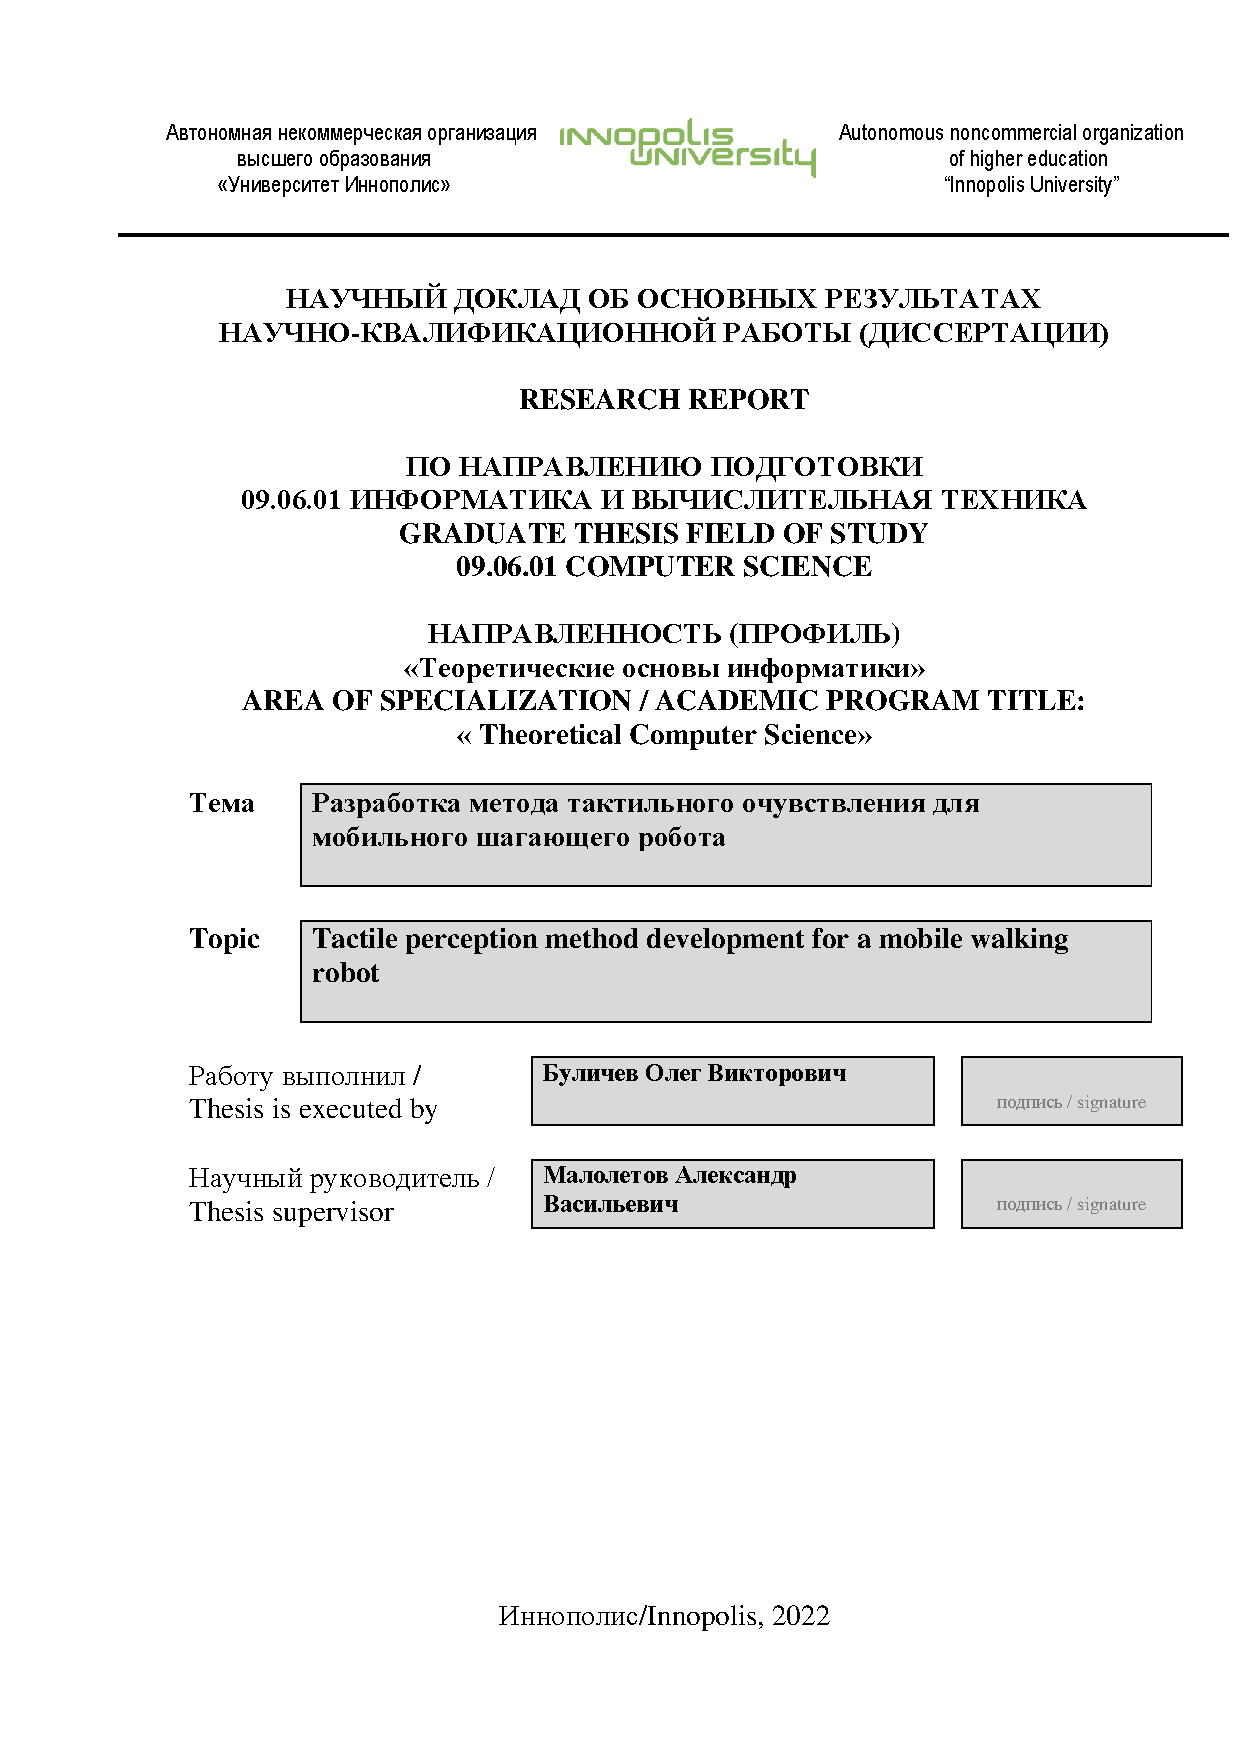
\includepdf[pages=-]{Titles_inno/synopsis_title.pdf}
% 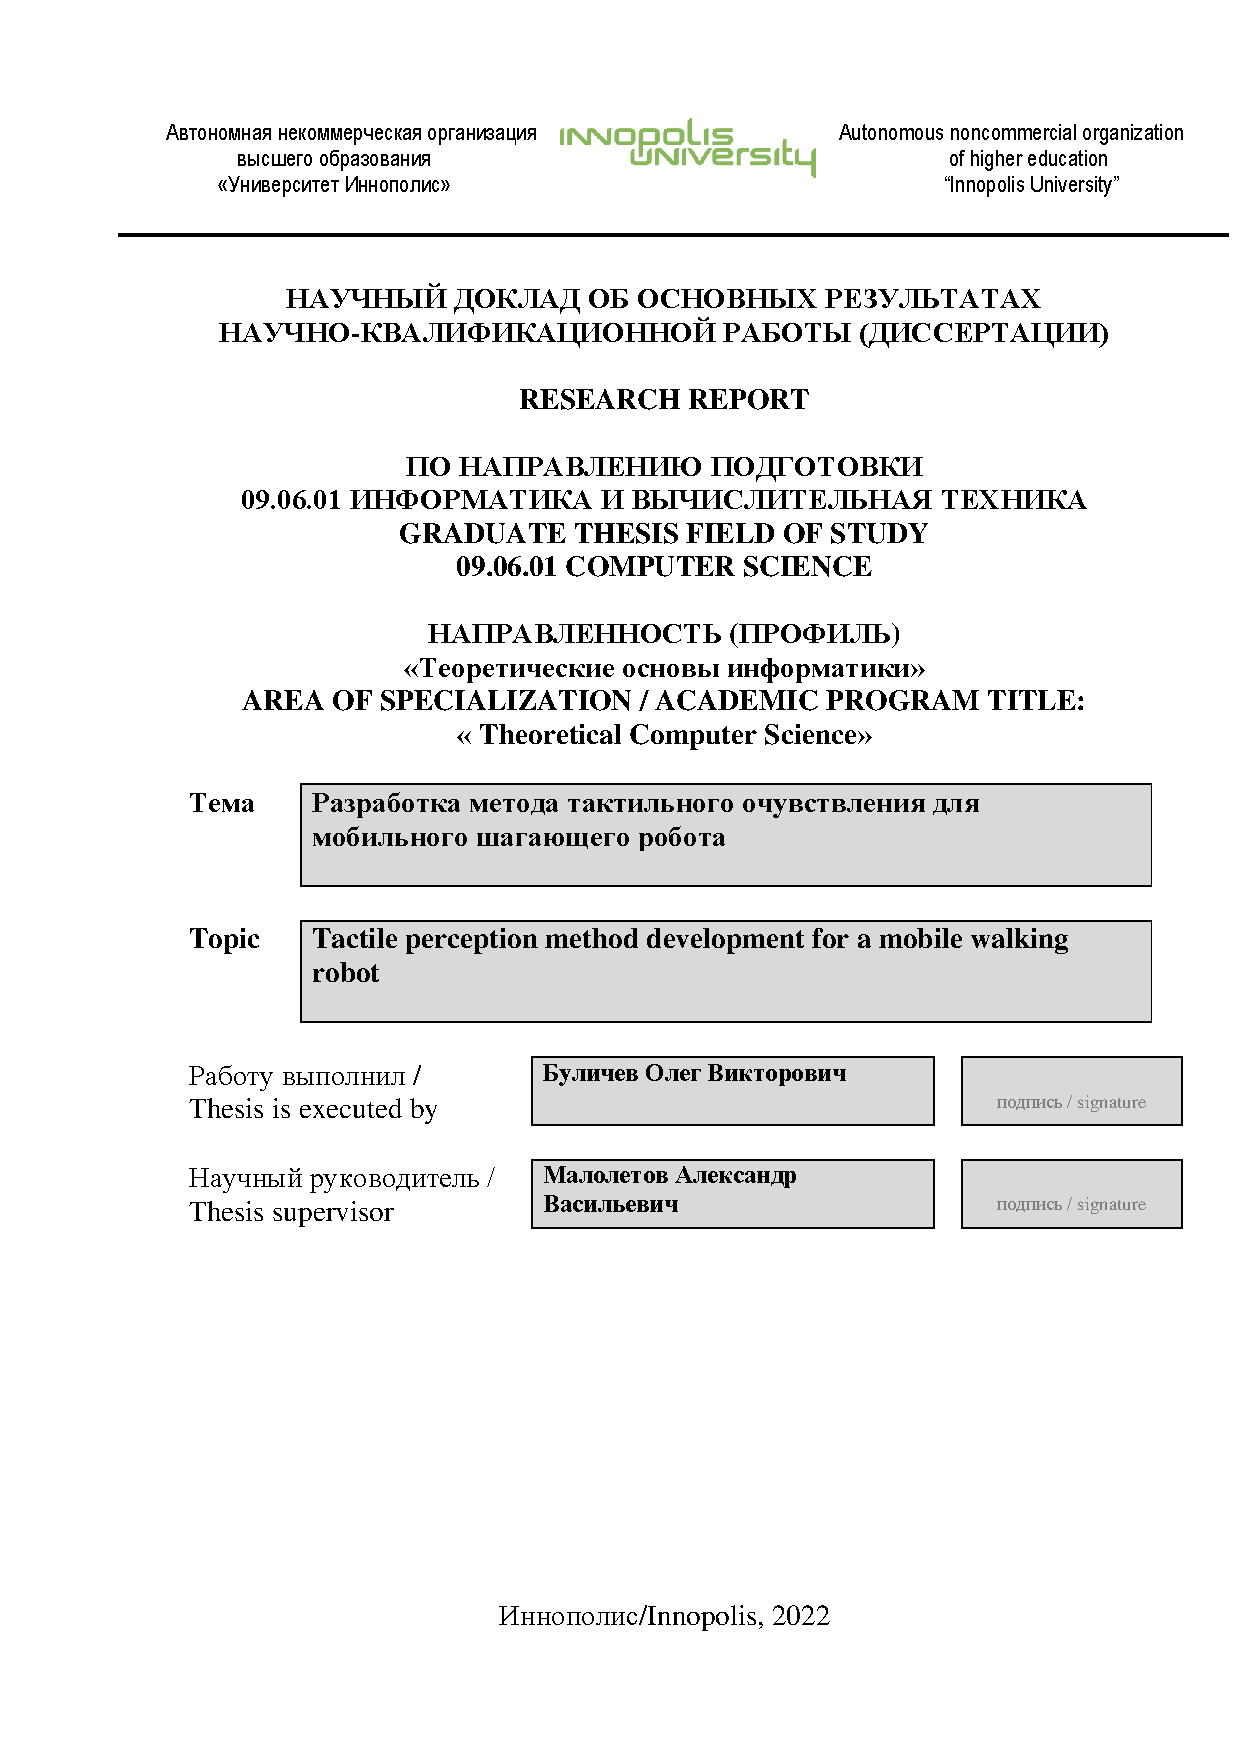
\includepdf[pages=-,fitpaper]{Titles_inno/synopsis_title.pdf}
\thispagestyle{empty}

\noindent%
% \begin{tabularx}{\textwidth}{@{}lXr@{}}%
%     & & \large{На правах рукописи}\\
%     \IfFileExists{images/logo.pdf}{\includegraphics[height=2.5cm]{logo}}{\rule[0pt]{0pt}{2.5cm}}  & &
%     \ifnumequal{\value{showperssign}}{0}{%
%         \rule[0pt]{0pt}{1.5cm}
%     }{
%         
\includegraphics[height=1.5cm]{personal-signature.png}
%     }\\
% \end{tabularx}

\vspace{0pt plus1fill} %число перед fill = кратность относительно некоторого расстояния fill, кусками которого заполнены пустые места
\begin{center}
\textbf {\large \thesisAuthor}
\end{center}

\vspace{0pt plus3fill} %число перед fill = кратность относительно некоторого расстояния fill, кусками которого заполнены пустые места
\begin{center}
\textbf {\Large %\MakeUppercase
\thesisTitle}

\vspace{0pt plus3fill} %число перед fill = кратность относительно некоторого расстояния fill, кусками которого заполнены пустые места
{\large \thesisSpecialtyNumber\ "\par \thesisSpecialtyTitle}

\ifdefined\thesisSpecialtyTwoNumber
{\large Специальность \thesisSpecialtyTwoNumber\ "---\par <<\thesisSpecialtyTwoTitle>>}
\fi

\vspace{0pt plus1.5fill} %число перед fill = кратность относительно некоторого расстояния fill, кусками которого заполнены пустые места
\Large{Автореферат}\par
\large{диссертации на соискание учёной степени\par \thesisDegree}
\end{center}

\vspace{0pt plus4fill} %число перед fill = кратность относительно некоторого расстояния fill, кусками которого заполнены пустые места
{\centering\thesisCity~--- \thesisYear\par}

\newpage
% оборотная сторона обложки
\thispagestyle{empty}
\noindent Работа выполнена в {\thesisInOrganization}.

\vspace{0.008\paperheight plus1fill}
\noindent%
\begin{tabularx}{\textwidth}{@{}lX@{}}
    \ifdefined\supervisorTwoFio
    Научные руководители   & \supervisorRegalia\par
                              \ifdefined\supervisorDead
                              \framebox{\textbf{\supervisorFio}}
                              \else
                              \textbf{\supervisorFio}
                              \fi
                              \par
                              \vspace{0.013\paperheight}
                              \supervisorRegalia\par
                              \ifdefined\supervisorTwoDead
                              \framebox{\textbf{\supervisorTwoFio}}
                              \else
                              \textbf{\supervisorTwoFio}
                              \fi
                              \vspace{0.013\paperheight}\\
    \else
    Научный руководитель   & \supervisorRegalia\par
                              \ifdefined\supervisorDead
                              \framebox{\textbf{\supervisorFio}}.
                              \else
                              \textbf{\supervisorFio}.
                              \fi
                              \vspace{0.013\paperheight}\\
    \fi
    Официальные оппоненты:  &
    \ifnumequal{\value{showopplead}}{0}{\vspace{13\onelineskip plus1fill}}{%
        \textbf{\opponentOneFio,}\par
        \opponentOneRegalia,\par
        \opponentOneJobPlace,\par
        \opponentOneJobPost\par
        \vspace{0.01\paperheight}
        \textbf{\opponentTwoFio,}\par
        \opponentTwoRegalia,\par
        \opponentTwoJobPlace,\par
        \opponentTwoJobPost
    \ifdefined\opponentThreeFio
        \par
        \vspace{0.01\paperheight}
        \textbf{\opponentThreeFio,}\par
        \opponentThreeRegalia,\par
        \opponentThreeJobPlace,\par
        \opponentThreeJobPost
    \fi
    }%
    \vspace{0.013\paperheight} \\
    \ifdefined\leadingOrganizationTitle
    Ведущая организация    &
    \ifnumequal{\value{showopplead}}{0}{\vspace{6\onelineskip plus1fill}}{%
        \leadingOrganizationTitle.
    }%
    \fi
\end{tabularx}
\vspace{0.008\paperheight plus1fill}

\noindent Защита состоится \defenseDate~на~заседании диссертационного совета \defenseCouncilNumber~, созданного на базе \defenseCouncilTitle~по адресу: \defenseCouncilAddress.

\vspace{0.008\paperheight plus1fill}
\noindent С диссертацией можно ознакомиться в библиотеке \synopsisLibrary.

%\vspace{0.008\paperheight plus1fill}
%\noindent Отзывы на автореферат в двух экземплярах, заверенные печатью учреждения, просьба направлять по адресу: \defenseCouncilAddress, ученому секретарю диссертационного совета~\defenseCouncilNumber.

\vspace{0.008\paperheight plus1fill}
\noindent{Автореферат разослан \synopsisDate.}

%\noindent Телефон для справок: \defenseCouncilPhone.

\vspace{0.008\paperheight plus1fill}
\noindent%
\begin{tabularx}{\textwidth}{@{}%
>{\raggedright\arraybackslash}b{18em}@{}
>{\centering\arraybackslash}X
r
@{}}
    Ученый секретарь\par
    диссертационного совета
    &
    \ifnumequal{\value{showsecrsign}}{0}{}{%
        
\includegraphics[width=2cm]{secretary-signature.png}%
    }%
    &
    \defenseSecretaryFio
\end{tabularx}
        % Титульный лист
%\mainmatter                   % В том числе начинает нумерацию страниц арабскими цифрами с единицы
\mainmatter*                  % Нумерация страниц не изменится, но начнётся с новой страницы


\pdfbookmark{Общая характеристика работы}{characteristic}             % Закладка pdf
\section*{Общая характеристика работы}

\newcommand{\actuality}{\pdfbookmark[1]{Актуальность}{actuality}\underline{\textbf{\actualityTXT}}}
\newcommand{\progress}{\pdfbookmark[1]{Разработанность темы}{progress}\underline{\textbf{\progressTXT}}}
\newcommand{\aim}{\pdfbookmark[1]{Цели}{aim}\underline{{\textbf\aimTXT}}}
\newcommand{\tasks}{\pdfbookmark[1]{Задачи}{tasks}\underline{\textbf{\tasksTXT}}}
\newcommand{\aimtasks}{\pdfbookmark[1]{Цели и задачи}{aimtasks}\aimtasksTXT}
\newcommand{\novelty}{\pdfbookmark[1]{Научная новизна}{novelty}\underline{\textbf{\noveltyTXT}}}
\newcommand{\influence}{\pdfbookmark[1]{Практическая значимость}{influence}\underline{\textbf{\influenceTXT}}}
\newcommand{\methods}{\pdfbookmark[1]{Методология и методы исследования}{methods}\underline{\textbf{\methodsTXT}}}
\newcommand{\defpositions}{\pdfbookmark[1]{Положения, выносимые на защиту}{defpositions}\underline{\textbf{\defpositionsTXT}}}
\newcommand{\reliability}{\pdfbookmark[1]{Достоверность}{reliability}\underline{\textbf{\reliabilityTXT}}}
\newcommand{\probation}{\pdfbookmark[1]{Апробация}{probation}\underline{\textbf{\probationTXT}}}
\newcommand{\contribution}{\pdfbookmark[1]{Личный вклад}{contribution}\underline{\textbf{\contributionTXT}}}
\newcommand{\publications}{\pdfbookmark[1]{Публикации}{publications}\underline{\textbf{\publicationsTXT}}}

\newcommand{\struct}{\pdfbookmark[1]{Структура работы}{struct}\underline{\textbf{\structTXT}}}
\newcommand{\researchobj}{\pdfbookmark[1]{Объект исследования}{researchobj}\underline{\textbf{\researchobjTXT}}}
% \setcounter{page}{1}
{\actuality} Движение по пещере часто происходит по опасными и труднопроходимыми участкам. Наиболее опасными являются сифоны \pic{fig:surface_types/syphon}, сталактиты, сталагмиты, обилие скользких грунтов \pic{fig:surface_types/ice, fig:surface_types/moss, fig:surface_types/clay}. В пещерах недостаток света, часто влажно. Встречаются участки, покрытые водой \pic{fig:surface_types/splash} и растительностью \pic{fig:surface_types/moss}.

\begin{figure}[ht]
  \begin{subfigure}[b]{0.3\textwidth}
      \centering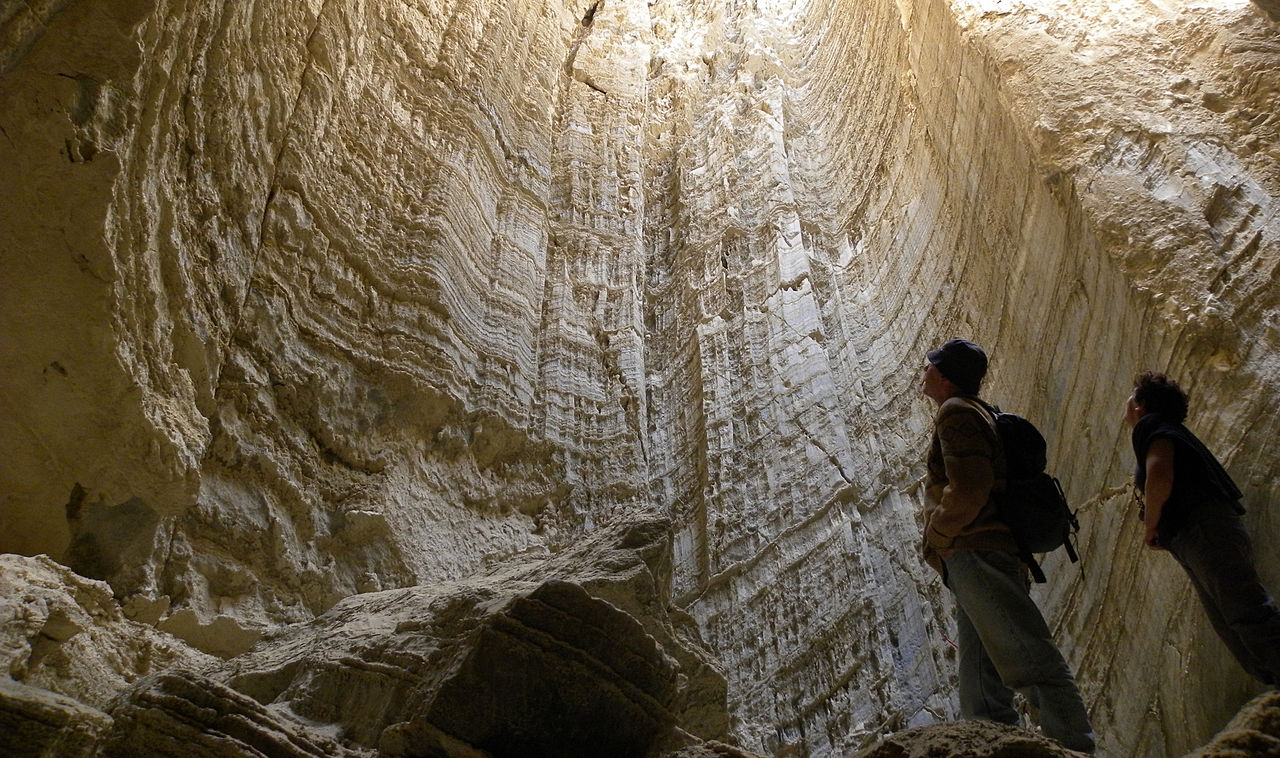
\includegraphics[height=2.8cm,width=1\textwidth,keepaspectratio]{surface_types/salt.jpg}\\
      \caption{Соляные отложения}
      \label{fig:surface_types/salt}
  \end{subfigure}
  \hfill
  \begin{subfigure}[b]{0.3\textwidth}
      \centering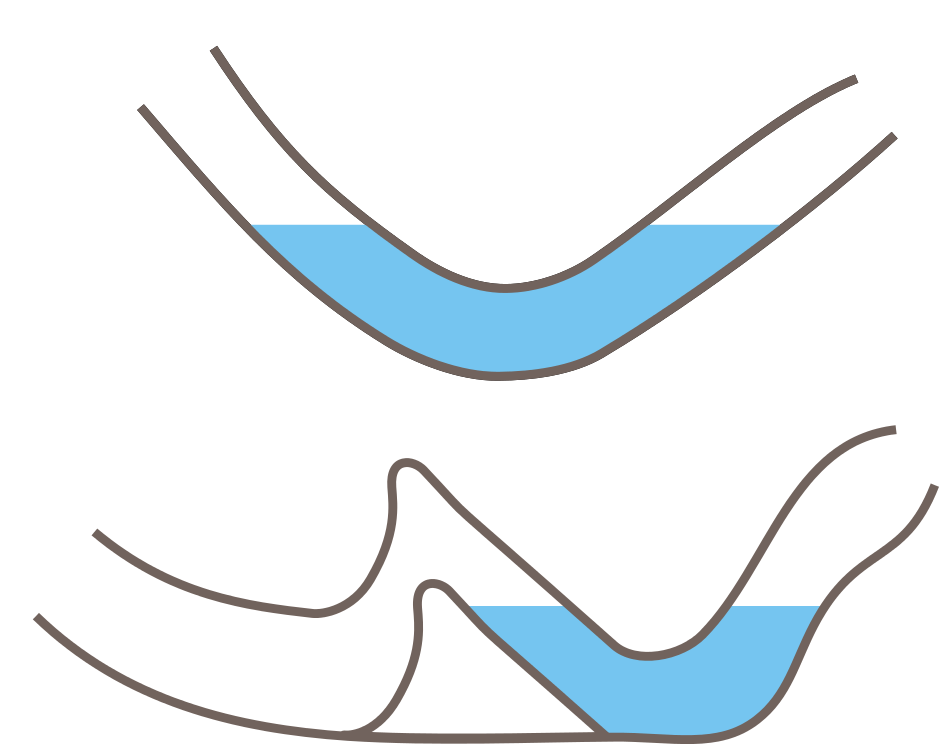
\includegraphics[height=2.8cm,width=1\textwidth,keepaspectratio]{surface_types/siphon.png}\\
      \caption{Сифон}
      \label{fig:surface_types/syphon}
  \end{subfigure}
  \hfill
  \begin{subfigure}[b]{0.3\textwidth}
      \centering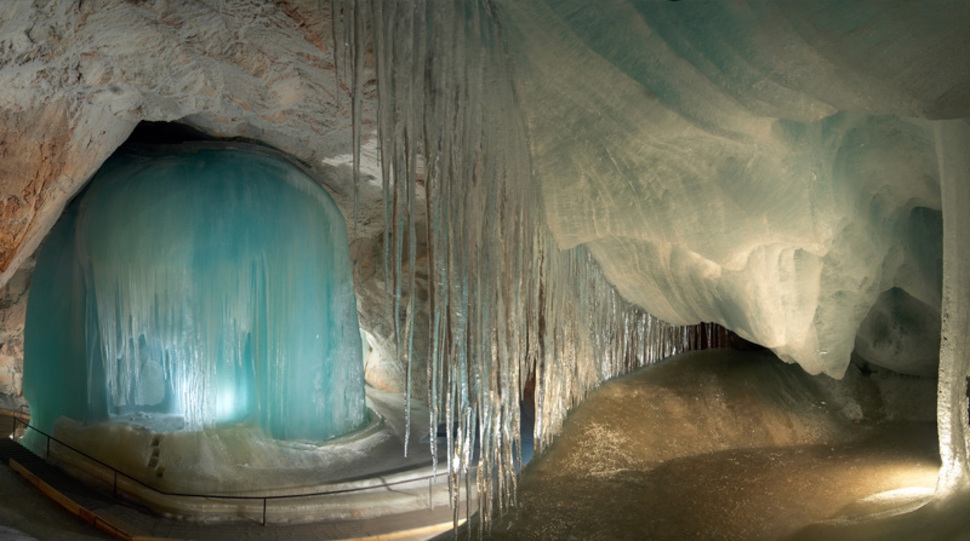
\includegraphics[height=2.8cm,width=1\textwidth,keepaspectratio]{surface_types/ice.png}\\
      \caption{Ледяная пещера}
      \label{fig:surface_types/ice}
  \end{subfigure}

  \begin{subfigure}[b]{0.3\textwidth}
      \centering
      \begin{tikzpicture}
          % Include the image in a node
          \node [above right, inner sep=0] (image) at (0,0)
          {\centering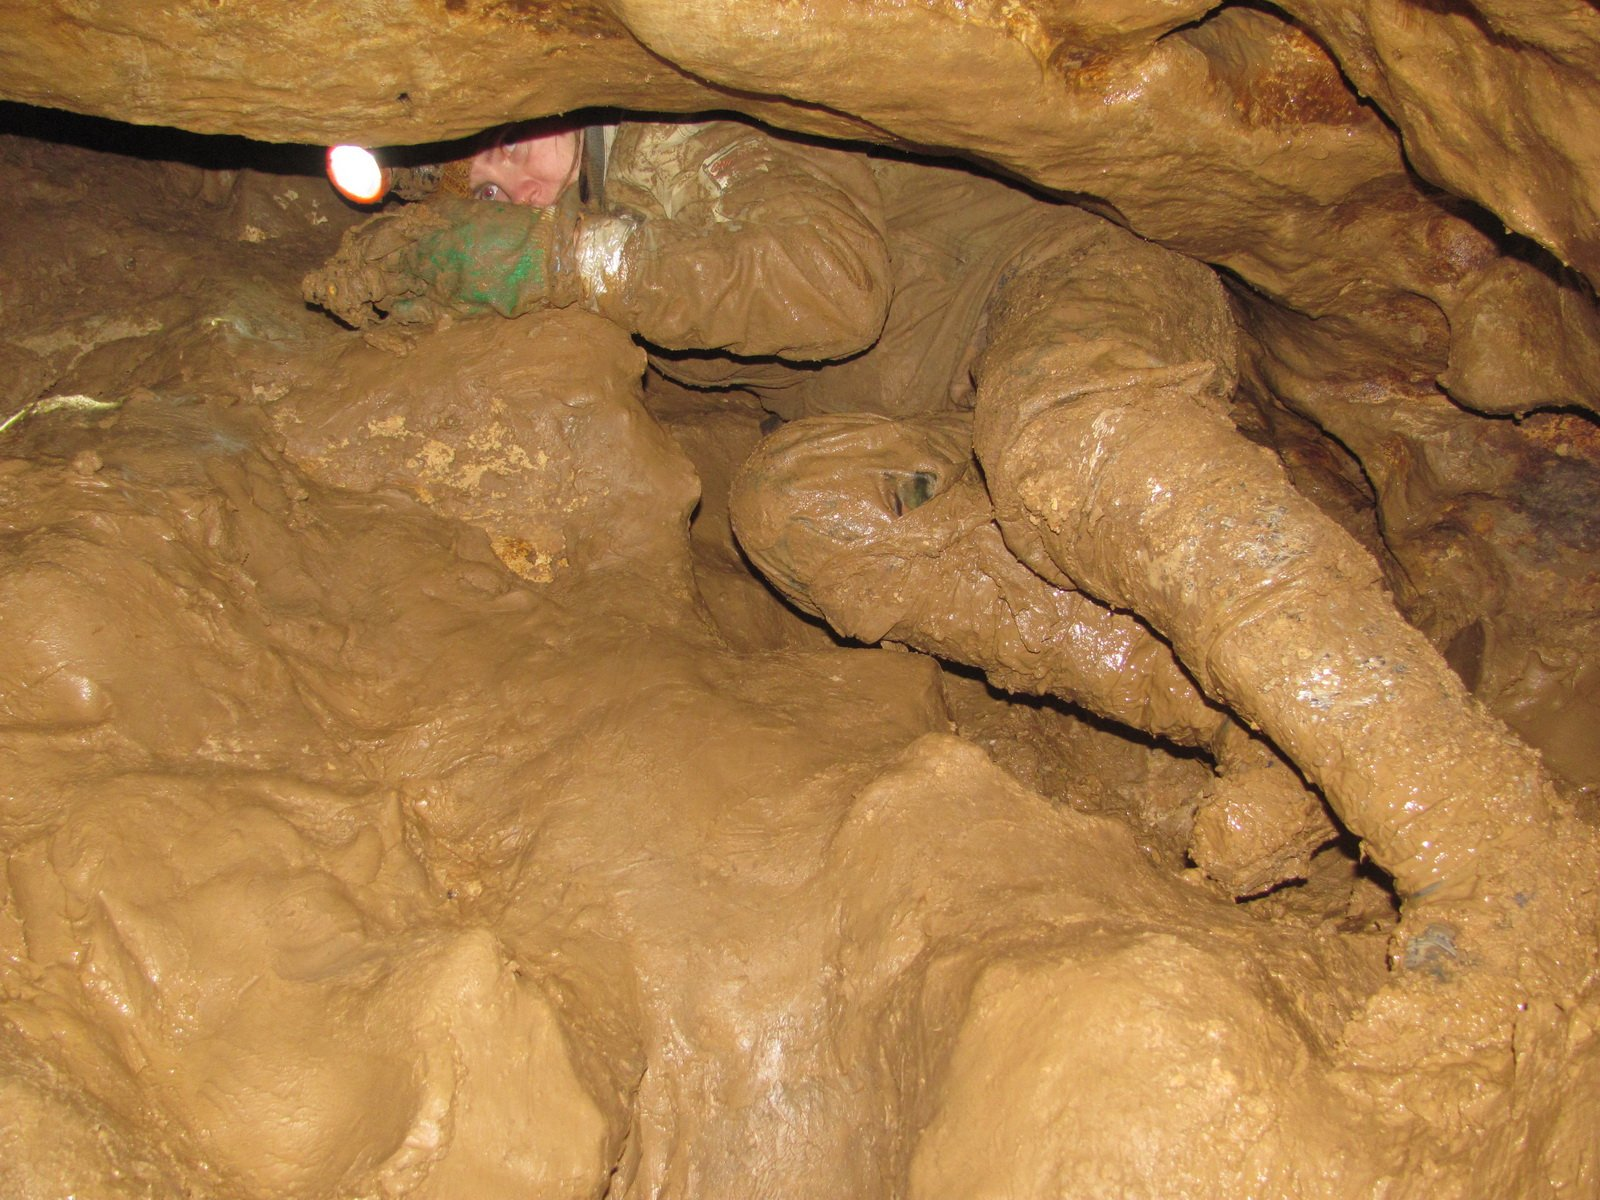
\includegraphics[height=2.8cm,width=1\textwidth,keepaspectratio]{surface_types/clay.jpg}};
          % Create scope with normalized axes
          \begin{scope}[
                  x={($ 0.1*(image.south east)$)},
                  y={($ 0.1*(image.north west)$)}]
              % Grid and axes' labels
              % \draw[lightgray,step=1] (image.south west) grid (image.north east);
              % \foreach \x in {0,1,...,10} { \node [below] at (\x,0) {\x}; }
              % \foreach \y in {0,1,...,10} { \node [left] at (0,\y) {\y};}
              % Labels
              \draw[stealth-, very thick,green] (6,8) -- ++(1,1)
              node[rounded corners=3pt,right,black,fill=white]{\tiny Человек};
          \end{scope}
      \end{tikzpicture}
      \caption{Глина}
      \label{fig:surface_types/clay}
  \end{subfigure}
  \hfill
  \begin{subfigure}[b]{0.3\textwidth}
      \centering
      \begin{tikzpicture}
          % Include the image in a node
          \node [above right, inner sep=0] (image) at (0,0)
          {\centering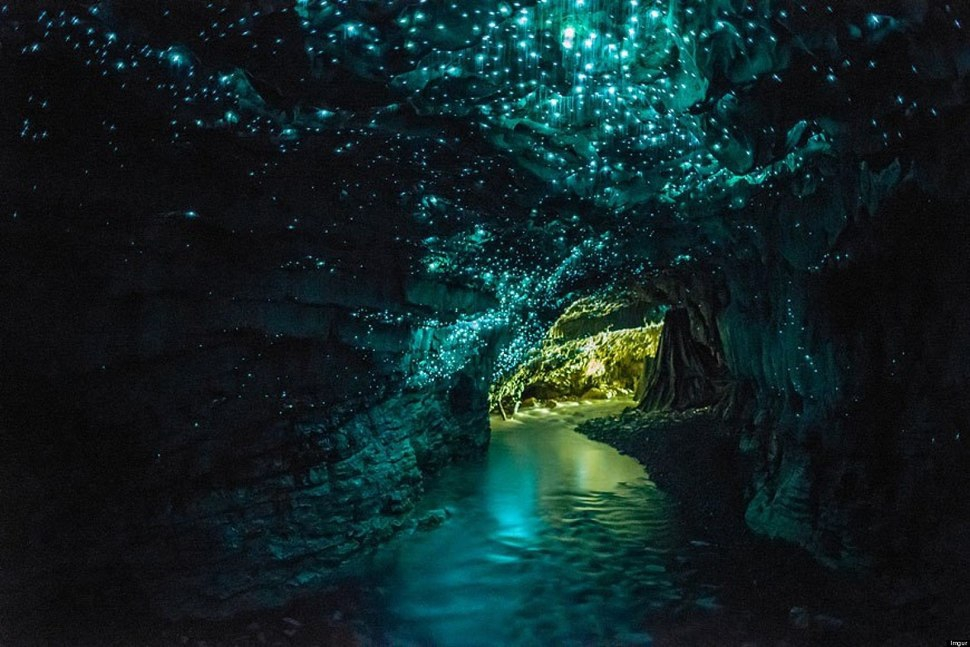
\includegraphics[height=2.8cm,width=1\textwidth,keepaspectratio]{surface_types/splash.png}};
          % Create scope with normalized axes
          \begin{scope}[
                  x={($ 0.1*(image.south east)$)},
                  y={($ 0.1*(image.north west)$)}]
              % Grid and axes' labels
              % \draw[lightgray,step=1] (image.south west) grid (image.north east);
              % \foreach \x in {0,1,...,10} { \node [below] at (\x,0) {\x}; }
              % \foreach \y in {0,1,...,10} { \node [left] at (0,\y) {\y};}

              % Labels
              \draw[stealth-, very thick,green] (5,2) -- ++(-2,+1)
              node[rounded corners=3pt,left,black,fill=white]{\tiny Лужа};
          \end{scope}
      \end{tikzpicture}
      \caption{Пещера, заполненная водой по~колено}
      \label{fig:surface_types/splash}
  \end{subfigure}
  \hfill
  \begin{subfigure}[b]{0.3\textwidth}
      \centering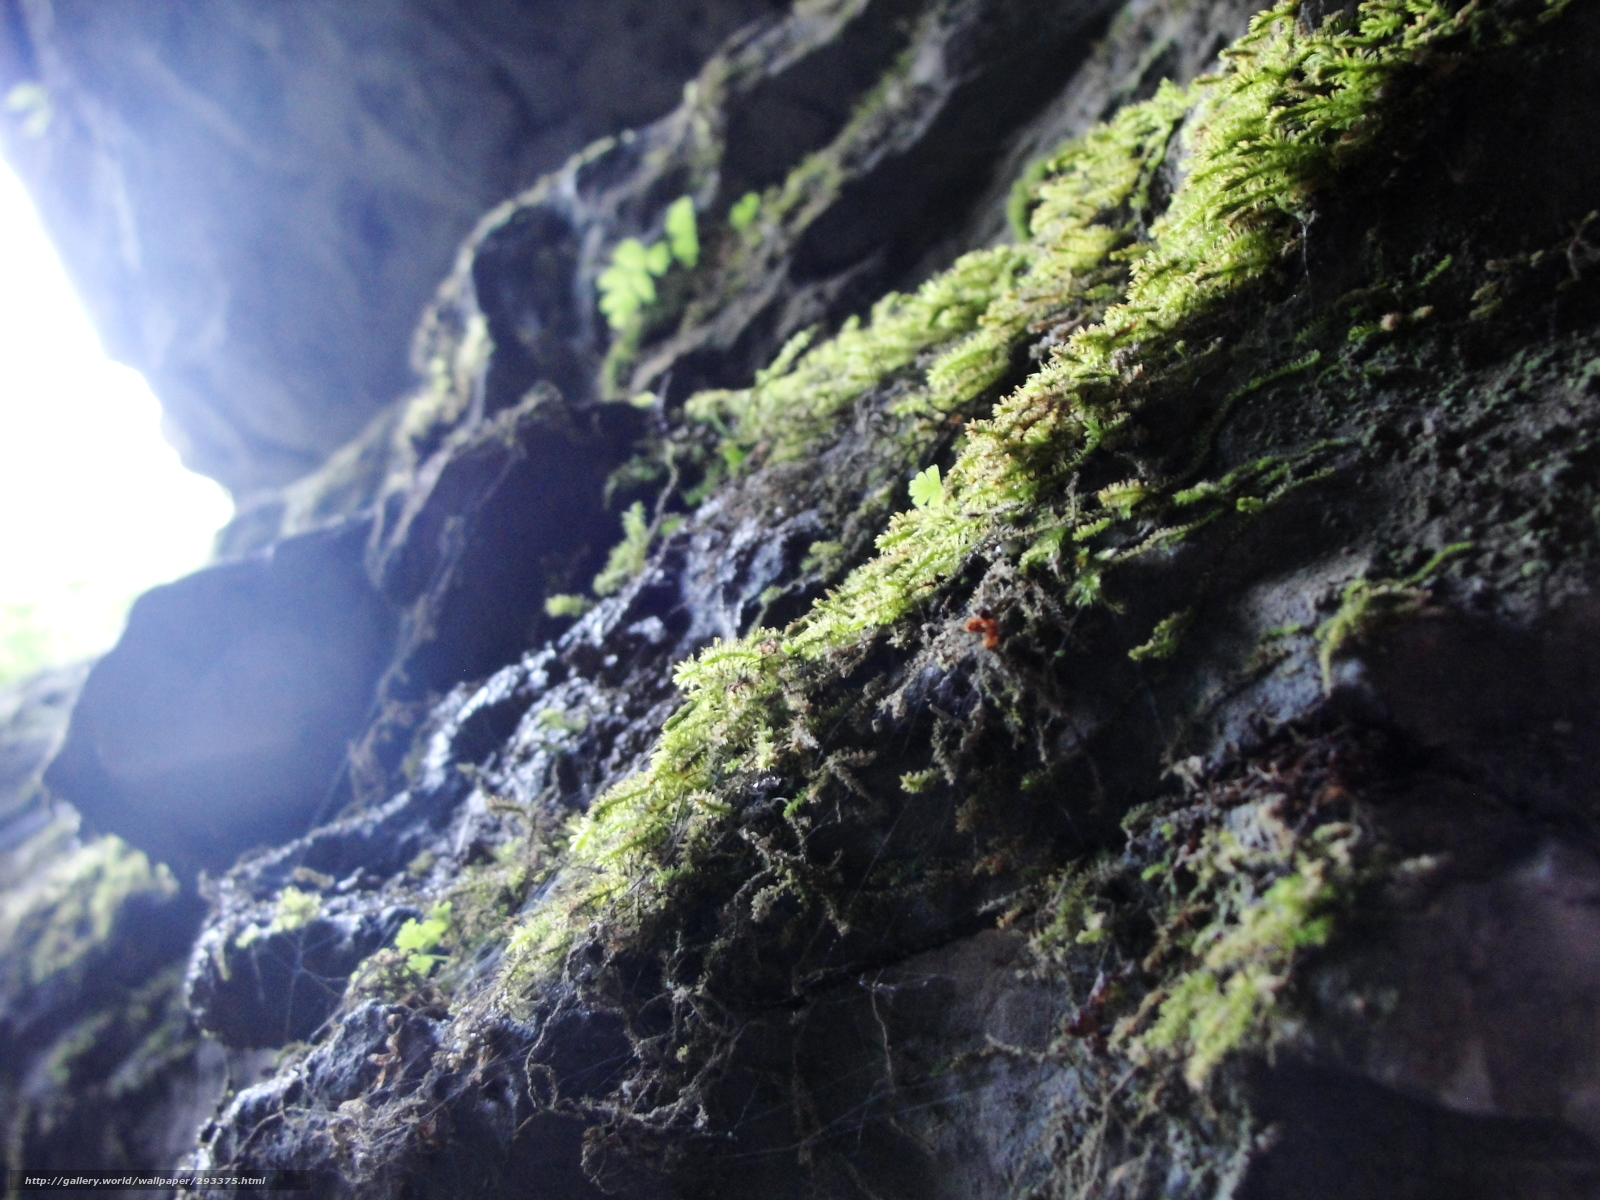
\includegraphics[height=2.8cm,width=1\textwidth,keepaspectratio]{surface_types/moss.jpg}\\
      \caption{Мох}
      \label{fig:surface_types/moss}
  \end{subfigure}
  \caption{Препятствия, встречающиеся в пещерах}\label{fig:obstacles}
\end{figure}


Эти препятствия могут встретиться человеком при исследовании или инспекции пещеры. Одно из преимуществ роботов --- они могут работать в опасных средах без нахождения рядом человека. Таким образом использование роботов в пещерах нивелирует все опасности для человека.

Существуют различные типы движителей роботов. С препятствиями представленными выше лучше всего справляются многоногие шагающие роботы. Такие роботы могут проходить по сыпучим грунтам, каменистым грядам и преодолевать небольшие водные преграды.

Для полноценного функционирования в пещере необходимы сенсоры. Внешними сенсорами являются камера и лидар.

Характерные для пещеры условия могут вывевсти из строя сенсоры. К примеру грязь \pic{fig:surface_types/clay} может закрыть обзор камере или лидару. Или водная гладь \pic{fig:surface_types/splash} будет отражать лучи лазера лидара и искажать данные \pic{fig:unsolvable_case}.

      \begin{figure}[h]
      \begin{subfigure}[t]{0.3\textwidth}
        \centering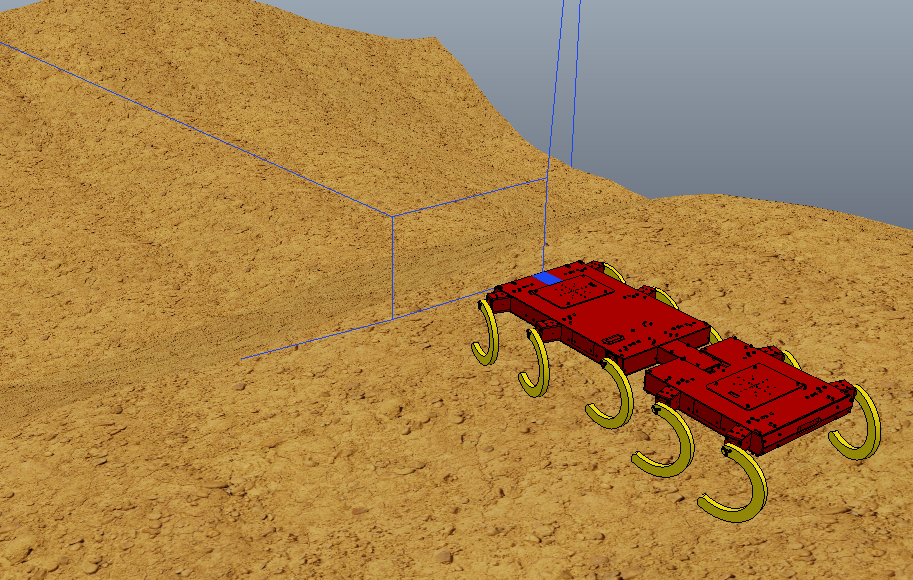
\includegraphics[height=3cm,width=1\textwidth,keepaspectratio]{terrain_wo_water.png}
        \caption{Территория без воды}
    \end{subfigure}
          \begin{subfigure}[t]{0.35\textwidth}
              \centering
              \begin{tikzpicture}
                  % Include the image in a node
                  \node [above right, inner sep=0] (image) at (0,0)
                  {\centering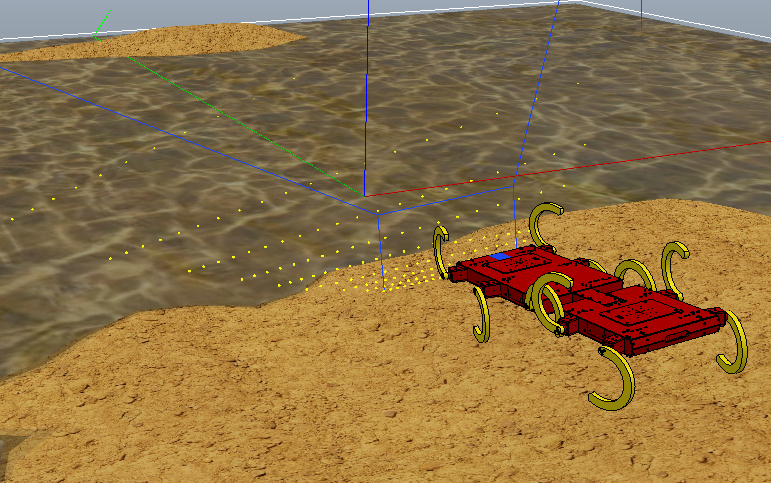
\includegraphics[height=3.5cm,width=1\textwidth,keepaspectratio]{terrain_w_water1.png}};
                  % Create scope with normalized axes
                  \begin{scope}[
                          x={($ 0.1*(image.south east)$)},
                          y={($ 0.1*(image.north west)$)}]
                      % Grid and axes' labels
                      \draw[stealth-, very thick,green] (6,8) -- ++(2,1)
                      node[rounded corners=3pt,right,black,fill=white]{\tiny Вода};

                      \draw[stealth-, very thick,green] (0.5,5.5) -- (3,2);
                      \draw[stealth-, very thick,green] (2.5,4.2) -- (3,2);
                      \draw[stealth-, very thick,green] (4.5,4) -- (3,2)
                      node[rounded corners=3pt,below,black,fill=white]{\tiny Данные с лидара};
                  \end{scope}
              \end{tikzpicture}
              \caption{Территория с водой}
              \label{fig:terrain_w_water1.png}
          \end{subfigure}
          \begin{subfigure}[t]{0.3\textwidth}
              \centering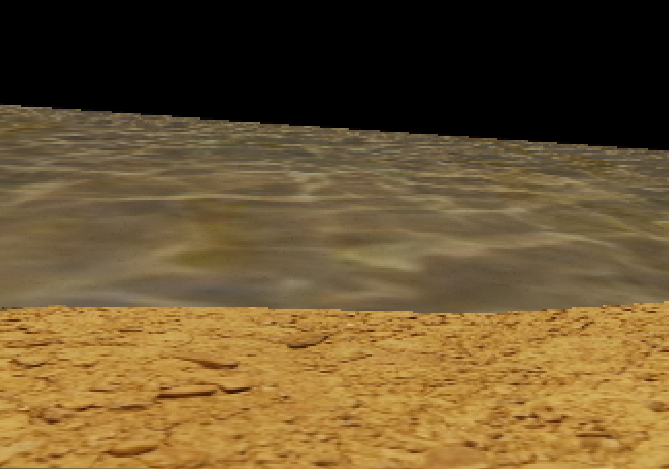
\includegraphics[height=3cm,width=1\textwidth,keepaspectratio]{terrain_w_water_camera.png}
              \caption{Изображение с камеры}
          \end{subfigure}
          \caption{Пример ситуации, где навигация, основанная на камере или лидаре построит неправильную карту}
          \label{fig:unsolvable_case}
      \end{figure}
  % \legend{Подрисуночный текст, описывающий обозначения, например. Согласно
  %     ГОСТ 2.105, пункт 4.3.1, располагается перед наименованием рисунка.}

% \ifsynopsis
% Этот абзац появляется только в~автореферате.
% Для формирования блоков, которые будут обрабатываться только в~автореферате,
% заведена проверка условия \verb!\!\verb!ifsynopsis!.
% Значение условия задаётся в~основном файле документа (\verb!synopsis.tex! для
% автореферата).
% \else
% Этот абзац появляется только в~диссертации.
% Через проверку условия \verb!\!\verb!ifsynopsis!, задаваемого в~основном файле
% документа (\verb!dissertation.tex! для диссертации), можно сделать новую
% команду, обеспечивающую появление цитаты в~диссертации, но~не~в~автореферате.
% \fi

{\aim} работы является разработка и исследование робототехнической системы построения карты местности и определения геометрических и физических свойств опорной поверхности на базе многоногого шагающего аппарата с тактильным очувствлением без использования оптических сенсоров.

Данное решение отлично подходит для первичного исследования замкнутых труднодоступных пространств, где отсутствует освещение, обилие грязи, пыли, а так же водных препятствий. Алгоритмы и концепты навигации данной системы могут быть использованы как резервная система навигации для других робототехнических систем, когда более точная --- оптическая вышла из строя.

Для~достижения поставленной цели решаются следующие {\tasks}:
\begin{enumerate}[beginpenalty=10000] % https://tex.stackexchange.com/a/476052/104425
    \item разрабатока метода оптимизации конструкции многоногих шагающих роботов с цикловыми движителями с одной степенью свободы по критериям проходимости (длина робота), детализации (количества ног), пройденного пути;
    \item создание методики исследования датчика силы, когда площадь контакта нажатия на сенсор меньше чувствительной области самого сенсора;
  \item  проектирование метода построения карты местности и определения поверхности с помощью тактильного очувствления;
  \item реализация алгоритма, позволяющего определять геометрические и физические свойства опорной поверхности.
\end{enumerate}

{\researchobj}
Объектом исследования является класс многоногих шагающих роботов с цельным или сочленённым корпусом, и цикловыми движителями с одной степенью свободы, управляемые зависимо или независимо друг от друга.

\begin{figure}[H]
  \centering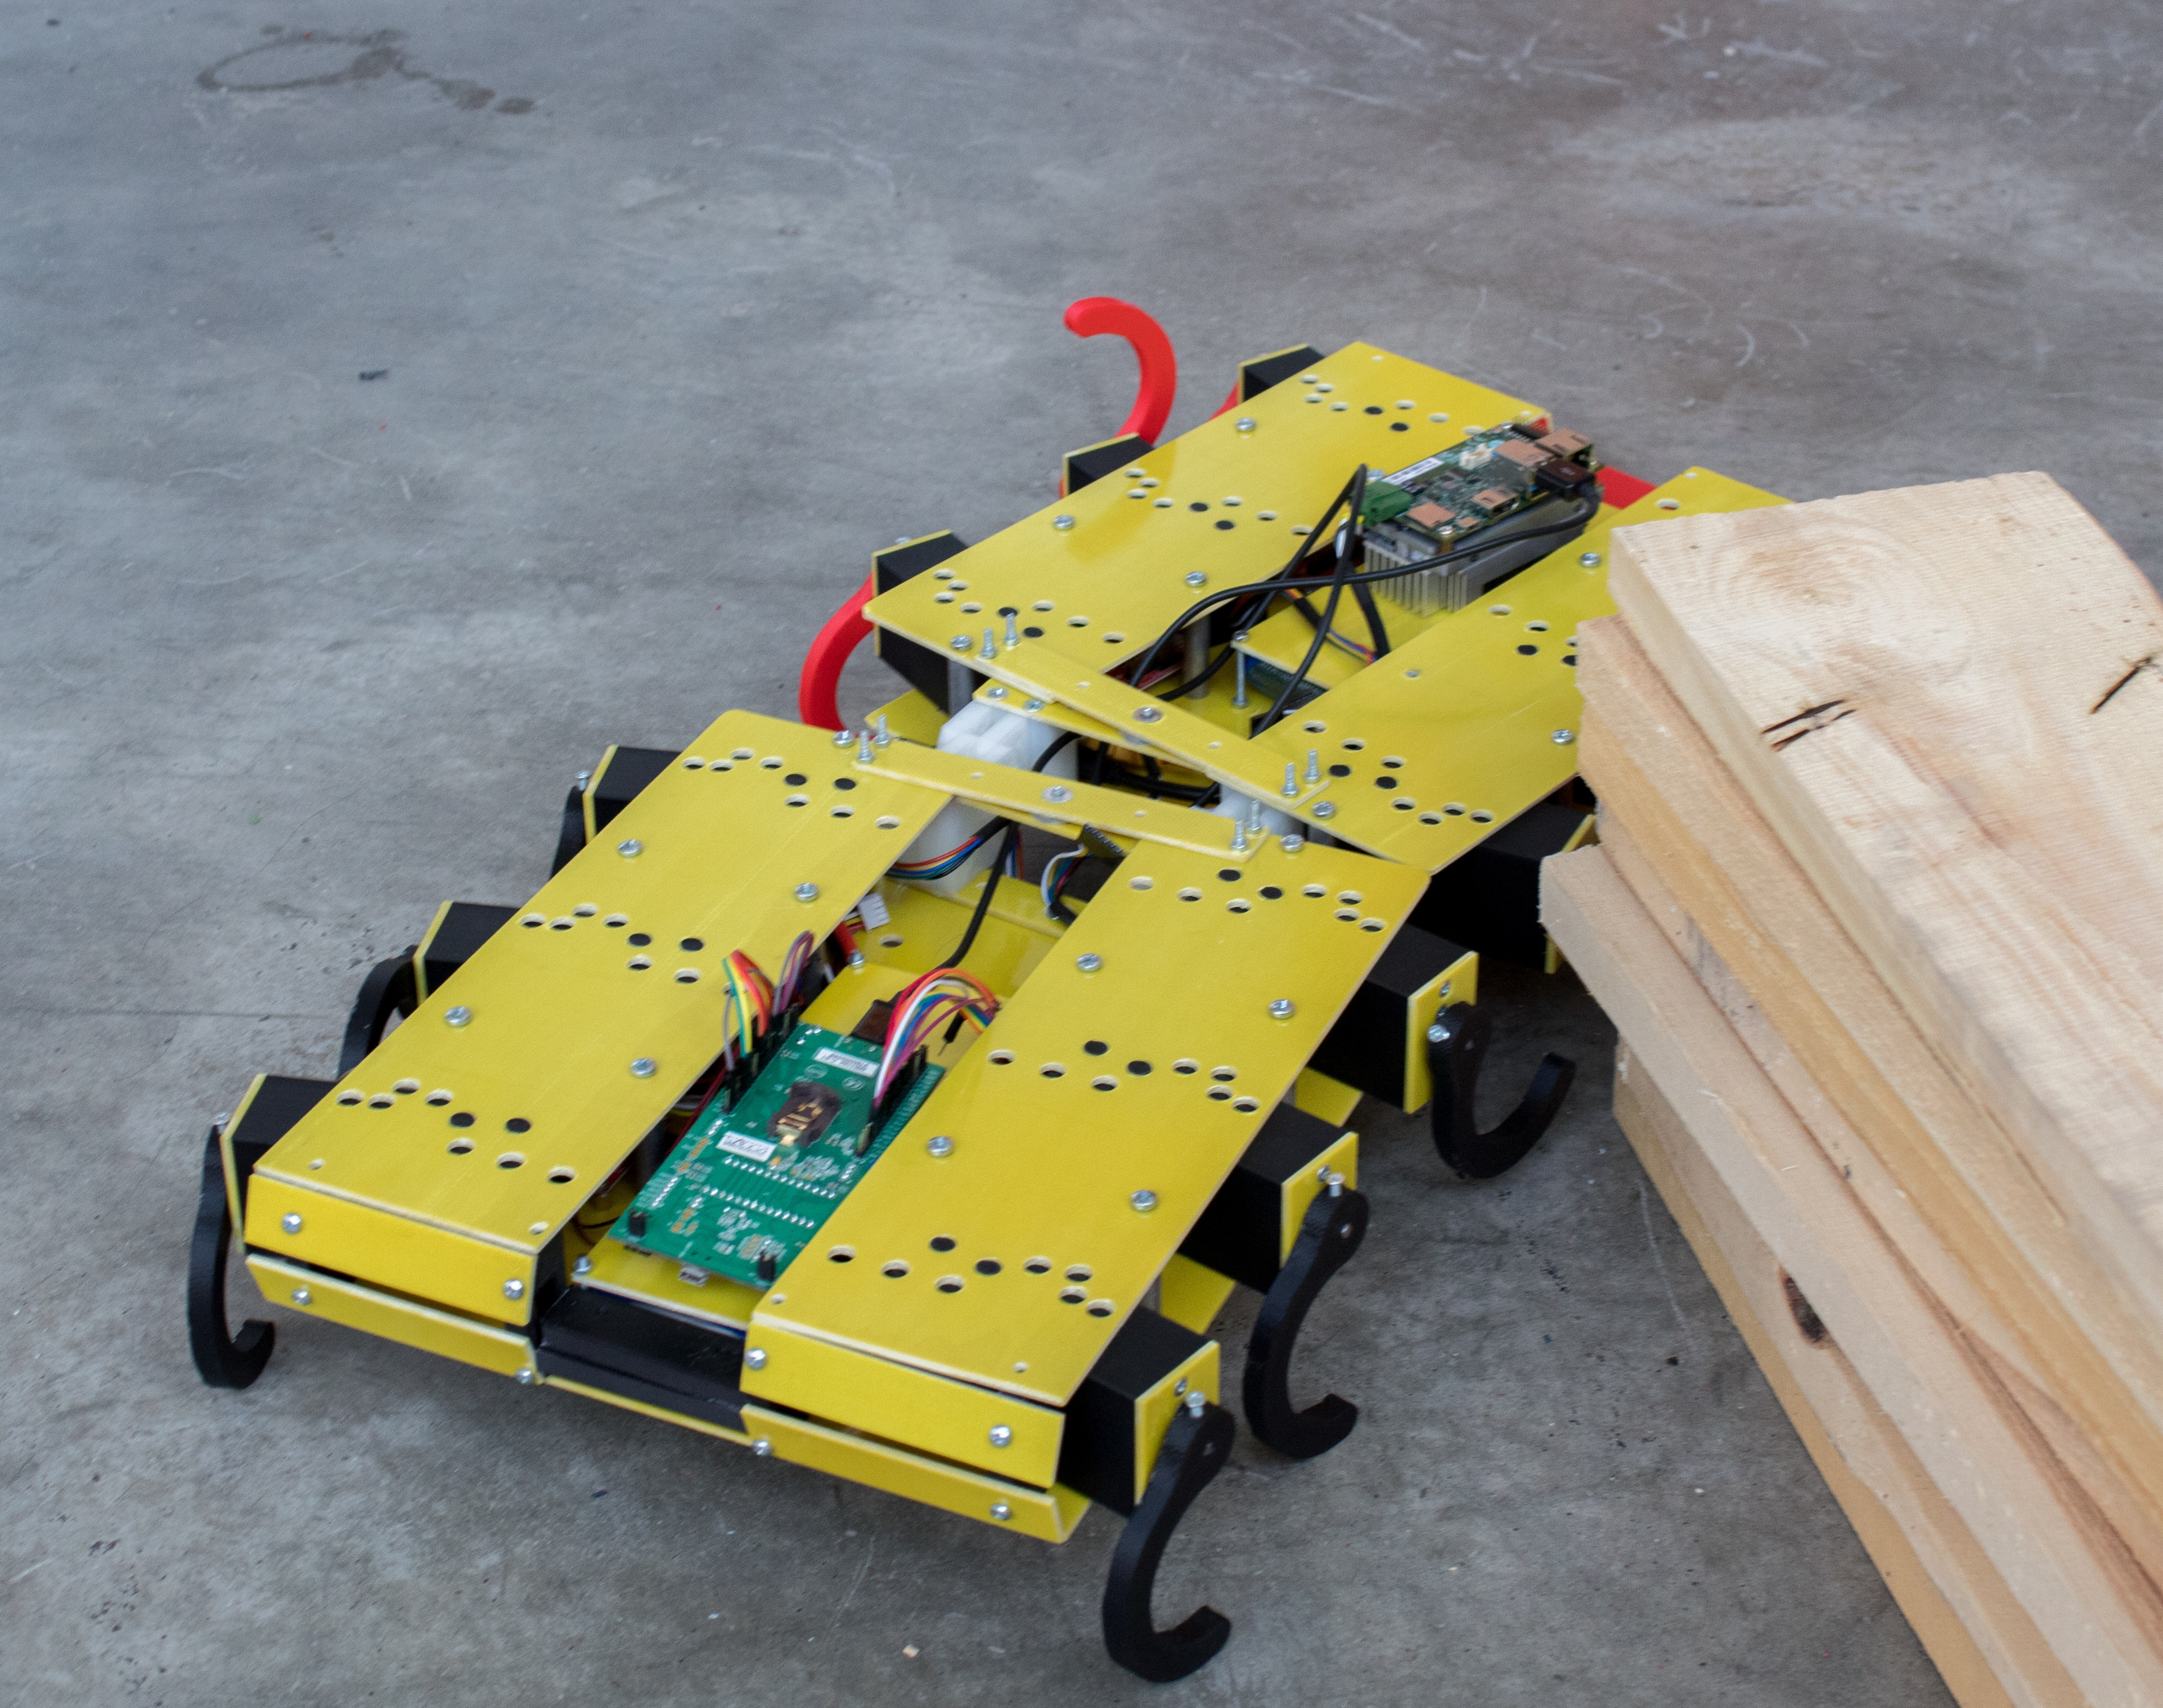
\includegraphics[height=7cm,width=1\textwidth,keepaspectratio]{strirus_2.jpg}
  \caption{Прототип, на котором было сделано большинство экспериментов}
  \label{fig:strirus_2.jpgg}
\end{figure}

Основная часть экспериментальных исследований проведена с прототипом \pic{fig:strirus_2.jpgg}, корпус которого состоит из двух сегментов с одной активной степенью свободы. Робот обладает 12 независимыми педипуляторами, 6 ног в первом сегменте и 6 во втором.

Особенность конструкции робота в том, что возможно изменять угол между ногой и корпусом робота. Данное конструктивное изменение позволило сделать перемещение робота всенаправленным, то есть робот может двигаться во все стороны без смены ориентации корпуса робота.


{\methods} За основу были взяты методологии из теории по разработке робототехнических систем, теоретической механики, механизмов и машин, теории оптимизации.

Для экспериментального исследования применялось численное и стендовое моделирования.

{\reliability} Правдивость результатов обеспечивается согласованностью с опубликованными результатами научных исследований других авторов, подтверждаются результатами компьютерного моделирования, натурными испытаниями. Результаты диссертационного исследования докладывались и обсуждались на российских и международных научных конференциях, и получили положительный отзыв научной общественности.


{\novelty} Сформулирована и решена задача построения карты местности с помощью тактильного очувствления шагающего робота с цикловыми движителями и датчиками силы, установленными на опорных поверхностях движителей.
Разработан метод оптимизации конструкции многоногого шагающего робота с цикловыми движителями. 
Разработана методика автоматизированного исследования датчика силы.


\textbf{Доказана} возможность построения карты местности и определения типа поверхности с помощью тактильного очувствления как в робототехническом симуляторе, так с помощью натурного эксперимента.

\textbf{Показано}, что оптимальное количество ног для циклового движителя с одной степенью свободы в ноге находится в диапазоне от 8 до 14 ног. 

\textbf{Предложено} использовать преобразователь силы на основе полимерного материала Velostat. \textbf{Установлено}, что данный преобразователь можно использовать для изначальной задачи, то есть при площади контакта с поверхностью большей, чем 25\% площади сенсора. 

\textbf{Сделан вывод} об эффективности предложенных методик, на основе результатов натурных испытаний.

{\defpositions}
\begin{enumerate}[beginpenalty=10000] % https://tex.stackexchange.com/a/476052/104425
  \item метод оптимизации конструкции многоногих шагающих роботов с цикловыми движителями с одной степенью свободы по критериям проходимости (длина робота), детализации (количества ног), пройденного пути;
  \item метод исследования датчика силы, когда площадь соприкосновения меньше площади сенсора;
  \item алгоритм, позволяющий определять тип поверхности;
  \item метод построения карты местности с помощью датчиков силы, установленных на ногах робота.
\end{enumerate}


{\influence} Реализация полученных результатов в виде продукта позволит получать информацию о типе пройденной поверхности, а так же строить карту поверхности под небольшим слоем воды (лужа), там где лидар и камера не смогут выдать адекватный результат.


{\probation}
Основные результаты работы докладывались~на:
\begin{itemize}
  \item ICINCO 2017 --- 14th International Conference on Informatics in Control, Automation and Robotics (Madrid, Spain, 26-28 july 2017);
  \item IEEE International Conference on Robotics and Biomimetics, ROBIO 2017 (Macau, China, 5-8 december 2017);
  \item  международной  научно-практической  конференции  «Прогресс  транспортных 
  средств и систем» (г. Волгоград, 9-11 октября 2018 г.);
  \item 23rd IEEE FRUCT Conference (Bologna, Italy, 13-16 november 2018).
  \item XXXI международной конференции молодых ученых и студентов МИКМУС-2019 
  (г. Москва, 4-6 декабря 2019 г.);
  \item Международная конференция <<Зимняя Школа Робототехники в Сириусе --- 2022>> (г. Адлер, Россия, 25 января - 6 февраля 2022)
\end{itemize}

{\contribution} Все научные результаты диссертации, выдвигаемые для защиты, получены автором лично.

% Вставка кто сколько опубликовался
\ifsynopsis
\ifnumequal{\value{bibliosel}}{0}
{%%% Встроенная реализация с загрузкой файла через движок bibtex8. (При желании, внутри можно использовать обычные ссылки, наподобие `\cite{vakbib1,vakbib2}`).
    {\publications} Основные результаты по теме диссертации изложены
    в~XX~печатных изданиях,
    X из которых изданы в журналах, рекомендованных ВАК,
    X "--- в тезисах докладов.
}%
{%%% Реализация пакетом biblatex через движок biber
    \begin{refsection}[bl-author, bl-registered]
        % Это refsection=1.
        % Процитированные здесь работы:
        %  * подсчитываются, для автоматического составления фразы "Основные результаты ..."
        %  * попадают в авторскую библиографию, при usefootcite==0 и стиле `\insertbiblioauthor` или `\insertbiblioauthorgrouped`
        %  * нумеруются там в зависимости от порядка команд `\printbibliography` в этом разделе.
        %  * при использовании `\insertbiblioauthorgrouped`, порядок команд `\printbibliography` в нём должен быть тем же (см. biblio/biblatex.tex)
        %
        % Невидимый библиографический список для подсчёта количества публикаций:
        \printbibliography[heading=nobibheading, section=1, env=countauthorvak,          keyword=biblioauthorvak]%
        \printbibliography[heading=nobibheading, section=1, env=countauthorwos,          keyword=biblioauthorwos]%
        \printbibliography[heading=nobibheading, section=1, env=countauthorscopus,       keyword=biblioauthorscopus]%
        \printbibliography[heading=nobibheading, section=1, env=countauthorconf,         keyword=biblioauthorconf]%
        \printbibliography[heading=nobibheading, section=1, env=countauthorother,        keyword=biblioauthorother]%
        \printbibliography[heading=nobibheading, section=1, env=countregistered,         keyword=biblioregistered]%
        \printbibliography[heading=nobibheading, section=1, env=countauthorpatent,       keyword=biblioauthorpatent]%
        \printbibliography[heading=nobibheading, section=1, env=countauthorprogram,      keyword=biblioauthorprogram]%
        \printbibliography[heading=nobibheading, section=1, env=countauthor,             keyword=biblioauthor]%
        \printbibliography[heading=nobibheading, section=1, env=countauthorvakscopuswos, filter=vakscopuswos]%
        \printbibliography[heading=nobibheading, section=1, env=countauthorscopuswos,    filter=scopuswos]%
        %
        \nocite{*}%
        %
        {\publications} Основные результаты по теме диссертации изложены в~\arabic{citeauthor}~печатных изданиях,
        \arabic{citeauthorvak} из которых изданы в журналах, рекомендованных ВАК\sloppy%
        \ifnum \value{citeauthorscopuswos}>0%
            , \arabic{citeauthorscopuswos} "--- в~периодических научных журналах, индексируемых Web of~Science и Scopus\sloppy%
        \fi%
        \ifnum \value{citeauthorconf}>0%
            , \arabic{citeauthorconf} "--- в~тезисах докладов.
        \else%
            .
        \fi%
        \ifnum \value{citeregistered}=1%
            \ifnum \value{citeauthorpatent}=1%
                Зарегистрирован \arabic{citeauthorpatent} патент.
            \fi%
            \ifnum \value{citeauthorprogram}=1%
                Зарегистрирована \arabic{citeauthorprogram} программа для ЭВМ.
            \fi%
        \fi%
        \ifnum \value{citeregistered}>1%
            Зарегистрированы\ %
            \ifnum \value{citeauthorpatent}>0%
            \formbytotal{citeauthorpatent}{патент}{}{а}{}\sloppy%
            \ifnum \value{citeauthorprogram}=0 . \else \ и~\fi%
            \fi%
            \ifnum \value{citeauthorprogram}>0%
            \formbytotal{citeauthorprogram}{программ}{а}{ы}{} для ЭВМ.
            \fi%
        \fi%
        % К публикациям, в которых излагаются основные научные результаты диссертации на соискание учёной
        % степени, в рецензируемых изданиях приравниваются патенты на изобретения, патенты (свидетельства) на
        % полезную модель, патенты на промышленный образец, патенты на селекционные достижения, свидетельства
        % на программу для электронных вычислительных машин, базу данных, топологию интегральных микросхем,
        % зарегистрированные в установленном порядке.(в ред. Постановления Правительства РФ от 21.04.2016 N 335)
    \end{refsection}%
    \begin{refsection}[bl-author, bl-registered]
        % Это refsection=2.
        % Процитированные здесь работы:
        %  * попадают в авторскую библиографию, при usefootcite==0 и стиле `\insertbiblioauthorimportant`.
        %  * ни на что не влияют в противном случае
        \nocite{vakbib2}%vak
        \nocite{patbib1}%patent
        \nocite{progbib1}%program
        \nocite{bib1}%other
        \nocite{confbib1}%conf
    \end{refsection}%
        %
        % Всё, что вне этих двух refsection, это refsection=0,
        %  * для диссертации - это нормальные ссылки, попадающие в обычную библиографию
        %  * для автореферата:
        %     * при usefootcite==0, ссылка корректно сработает только для источника из `external.bib`. Для своих работ --- напечатает "[0]" (и даже Warning не вылезет).
        %     * при usefootcite==1, ссылка сработает нормально. В авторской библиографии будут только процитированные в refsection=0 работы.
}
% При использовании пакета \verb!biblatex! будут подсчитаны все работы, добавленные
% в файл \verb!biblio/author.bib!. Для правильного подсчёта работ в~различных
% системах цитирования требуется использовать поля:
% \begin{itemize}
%         \item \texttt{authorvak} если публикация индексирована ВАК,
%         \item \texttt{authorscopus} если публикация индексирована Scopus,
%         \item \texttt{authorwos} если публикация индексирована Web of Science,
%         \item \texttt{authorconf} для докладов конференций,
%         \item \texttt{authorpatent} для патентов,
%         \item \texttt{authorprogram} для зарегистрированных программ для ЭВМ,
%         \item \texttt{authorother} для других публикаций.
% \end{itemize}
% Для подсчёта используются счётчики:
% \begin{itemize}
%         \item \texttt{citeauthorvak} для работ, индексируемых ВАК,
%         \item \texttt{citeauthorscopus} для работ, индексируемых Scopus,
%         \item \texttt{citeauthorwos} для работ, индексируемых Web of Science,
%         \item \texttt{citeauthorvakscopuswos} для работ, индексируемых одной из трёх баз,
%         \item \texttt{citeauthorscopuswos} для работ, индексируемых Scopus или Web of~Science,
%         \item \texttt{citeauthorconf} для докладов на конференциях,
%         \item \texttt{citeauthorother} для остальных работ,
%         \item \texttt{citeauthorpatent} для патентов,
%         \item \texttt{citeauthorprogram} для зарегистрированных программ для ЭВМ,
%         \item \texttt{citeauthor} для суммарного количества работ.
% \end{itemize}
% % Счётчик \texttt{citeexternal} используется для подсчёта процитированных публикаций;
% % \texttt{citeregistered} "--- для подсчёта суммарного количества патентов и программ для ЭВМ.

% Для добавления в список публикаций автора работ, которые не были процитированы в
% автореферате, требуется их~перечислить с использованием команды \verb!\nocite! в
% \verb!Synopsis/content.tex!.

\fi

Диссертационная работа была выполнена при поддержке грантов:
\begin{itemize}
    \item НТИ по поддержке Центра <<Технологий Компонентов Робототехники и Мехатроники>> на базе Университета Иннополис по теме <<Разработка роботизированных платформ для автономной подземной и наземной инспекции местности в условиях трудной проходимости и плохой видимости>>. 
    \item РФФИ № 20-38-90265 по теме <<Разработка метода очувствления мобильного шагающего робота, перемещающегося в закрытом пространстве естественного происхождения>>.
\end{itemize}

{\struct}


% В введении рассказывается об актуальности проблемы, в чем научная новизна и цель проекта. Во первой главе показан обзор существующих решений. Вторая глава покрывает разработку объекта исследования, а именно решение задачи топологического синтеза и инженерную разработку прототипа. Третья глава посвящена разработке и исследованию самодельного преобразователя силы на основе Velostat. Четвертая глава раскрывает детали создания алгоритма построения карты с помощью тактильного очувствления, определения типа поверхности.
% Четвертая глава раскрывает детали создания алгоритма построения карты с помощью тактильного очувствления, решение проблемы локализации с помощью датчиков датчиков силы, IMU и маяков. Решатся проблема определения типа поверхности. % Характеристика работы по структуре во введении и в автореферате не отличается (ГОСТ Р 7.0.11, пункты 5.3.1 и 9.2.1), потому её загружаем из одного и того же внешнего файла, предварительно задав форму выделения некоторым параметрам



\pdfbookmark{Содержание работы}{description}                          % Закладка pdf
\section*{Содержание работы}
Рассматривались 3 глобальных темы: обзор препятствий, роботы, которые используются в исследованиях пещер, а так же методы построения карты местности.

\subsection{Обзор
препятствий}

Для решения поставленной цели необходимо понимать в каких условиях будет использоваться робот.

Пещера -- полость в верхней части земной коры, сообщающаяся с поверхностью одним или несколькими входными отверстиями. Они бывают различных типов, от этого зависит какой набор препятствий будет встречаться чаще.

Основные структуры поверхностей следующие \pic{fig:obstacles}:
\begin{itemize}
    \item твердые породы, прочные -- мрамор, кварц, базальт (магма);
    \item твердые породы, мягкие -- мел, гипс, соль, известняк;
    \item сыпучие грунты -- песок, глина, снег;
    \item водные преграды -- как и лужи (малый слой воды), так и целы залы, погруженные под воду. Часто встречаются сифоны;
    \item скользкие поверхности -- отложения мха и плесени, лед ;
    \item разрушаемые поверхности -- каменная гряда, паутина.
\end{itemize}

\begin{figure}[ht]
    \begin{subfigure}[b]{0.3\textwidth}
        \centering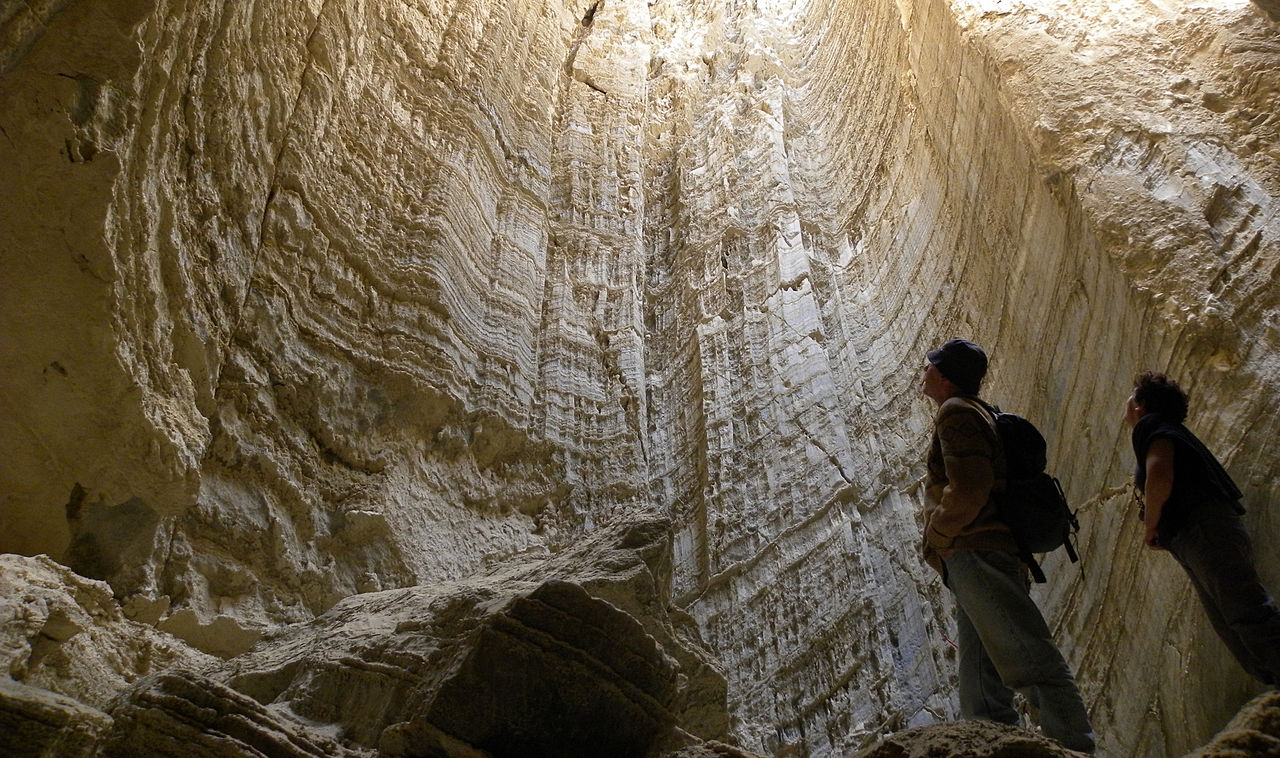
\includegraphics[height=2.8cm,width=1\textwidth,keepaspectratio]{surface_types/salt.jpg}\\
        \caption{Соляные отложения}
        \label{fig:surface_types/salt}
    \end{subfigure}
    \hfill
    \begin{subfigure}[b]{0.3\textwidth}
        \centering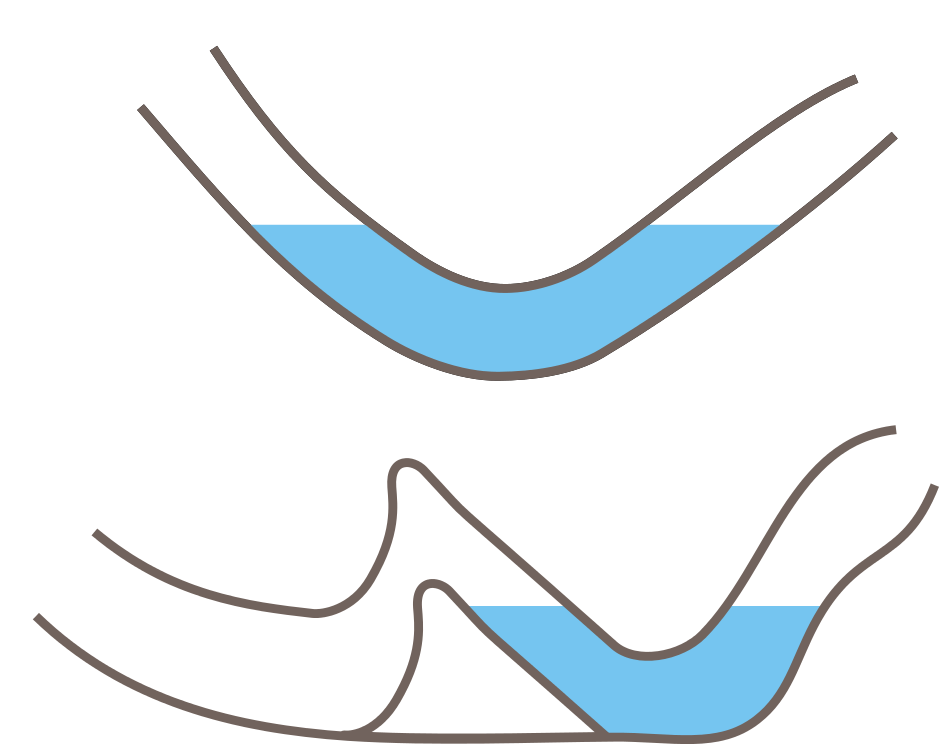
\includegraphics[height=2.8cm,width=1\textwidth,keepaspectratio]{surface_types/siphon.png}\\
        \caption{Сифон}
        \label{fig:surface_types/siphon}
    \end{subfigure}
    \hfill
    \begin{subfigure}[b]{0.3\textwidth}
        \centering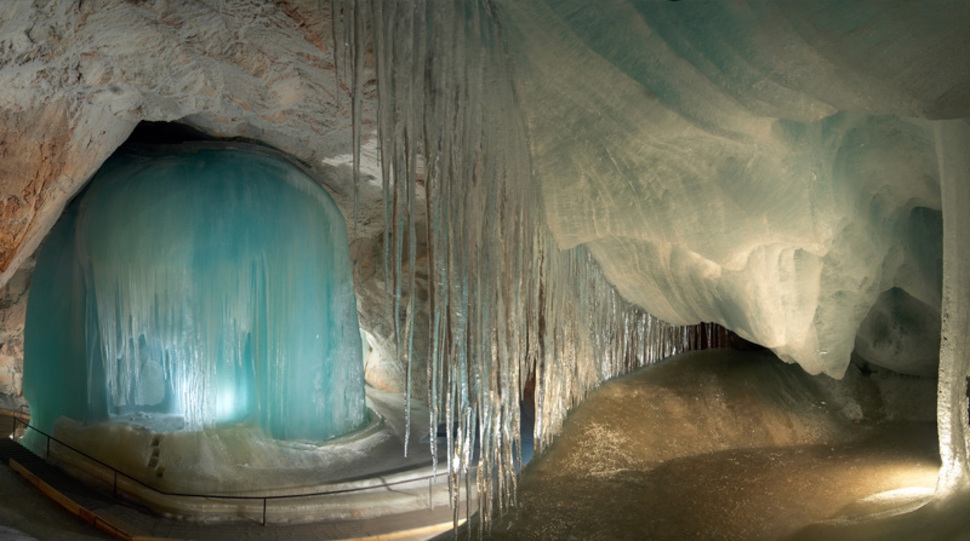
\includegraphics[height=2.8cm,width=1\textwidth,keepaspectratio]{surface_types/ice.png}\\
        \caption{Ледяная пещера}
        \label{fig:surface_types/ice}
    \end{subfigure}
  
    \begin{subfigure}[b]{0.3\textwidth}
        \centering
        \begin{tikzpicture}
            % Include the image in a node
            \node [above right, inner sep=0] (image) at (0,0)
            {\centering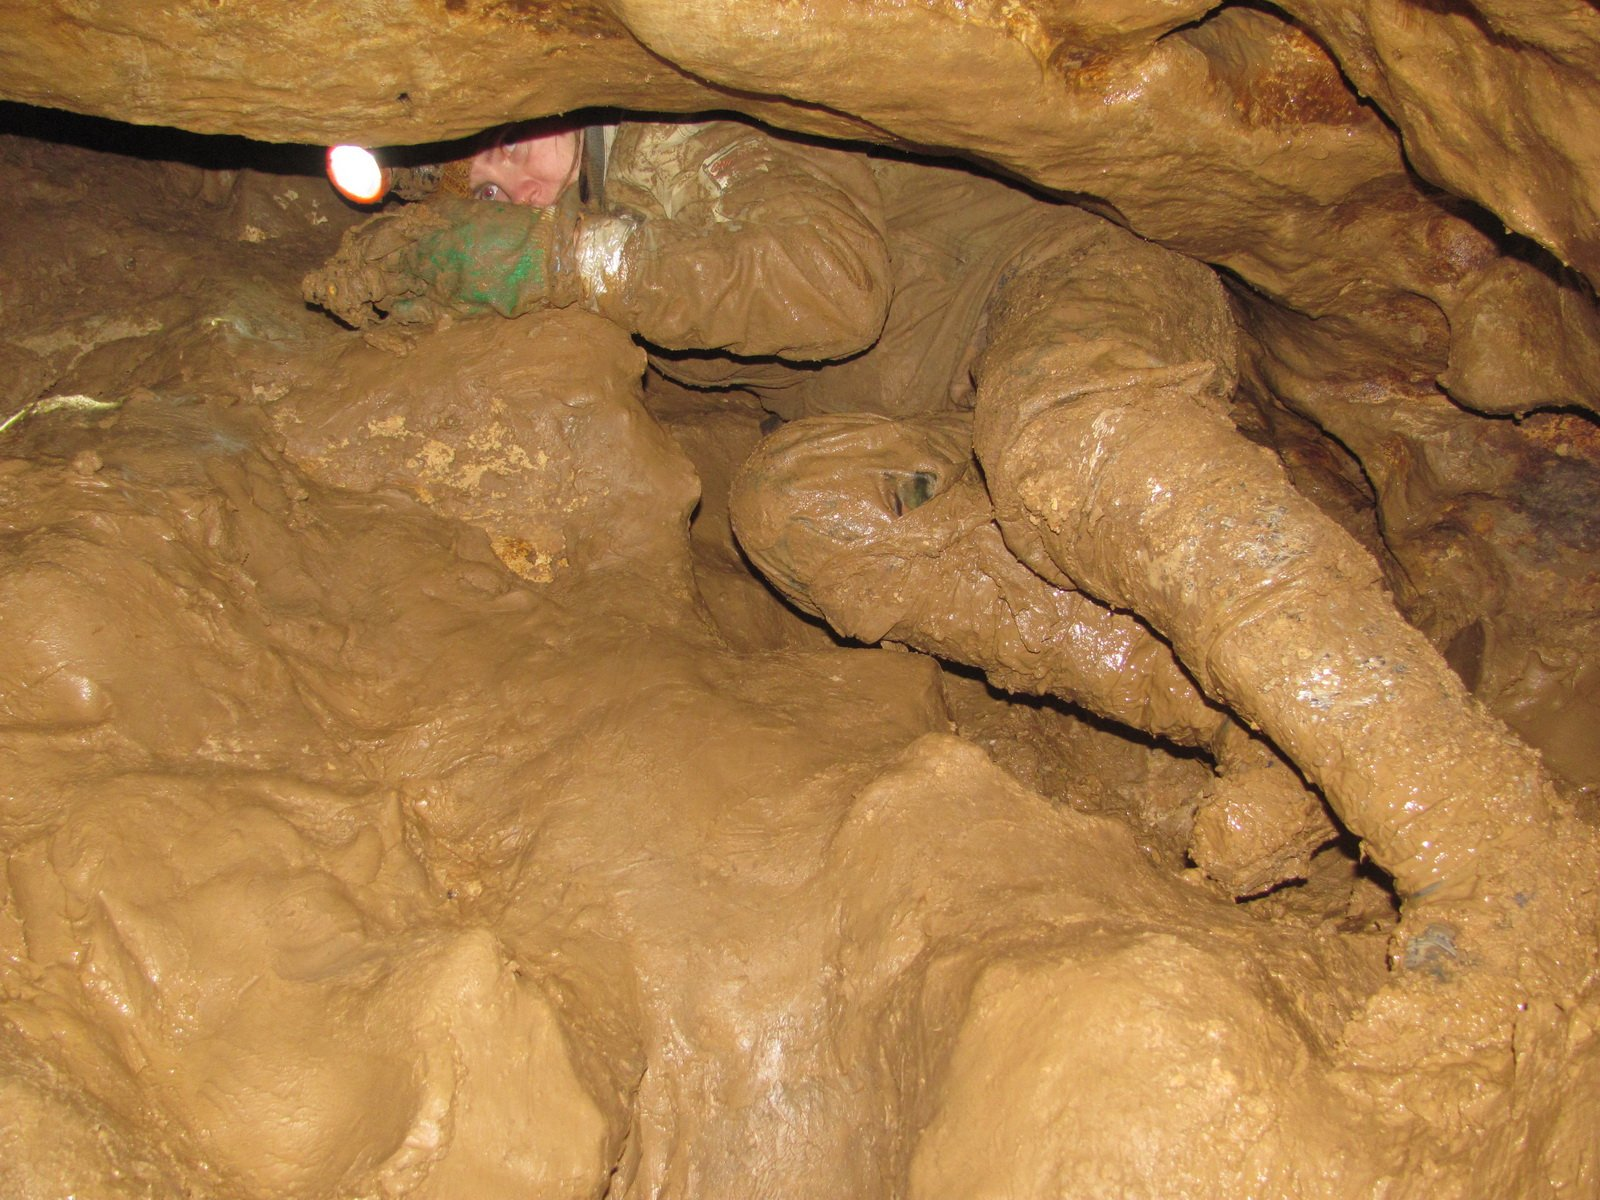
\includegraphics[height=2.8cm,width=1\textwidth,keepaspectratio]{surface_types/clay.jpg}};
            % Create scope with normalized axes
            \begin{scope}[
                    x={($ 0.1*(image.south east)$)},
                    y={($ 0.1*(image.north west)$)}]
                % Grid and axes' labels
                % \draw[lightgray,step=1] (image.south west) grid (image.north east);
                % \foreach \x in {0,1,...,10} { \node [below] at (\x,0) {\x}; }
                % \foreach \y in {0,1,...,10} { \node [left] at (0,\y) {\y};}
                % Labels
                \draw[stealth-, very thick,green] (6,8) -- ++(1,1)
                node[rounded corners=3pt,right,black,fill=white]{\tiny Человек};
            \end{scope}
        \end{tikzpicture}
        \caption{Глина}
        \label{fig:surface_types/clay.jpg}
    \end{subfigure}
    \hfill
    \begin{subfigure}[b]{0.3\textwidth}
        \centering
        \begin{tikzpicture}
            % Include the image in a node
            \node [above right, inner sep=0] (image) at (0,0)
            {\centering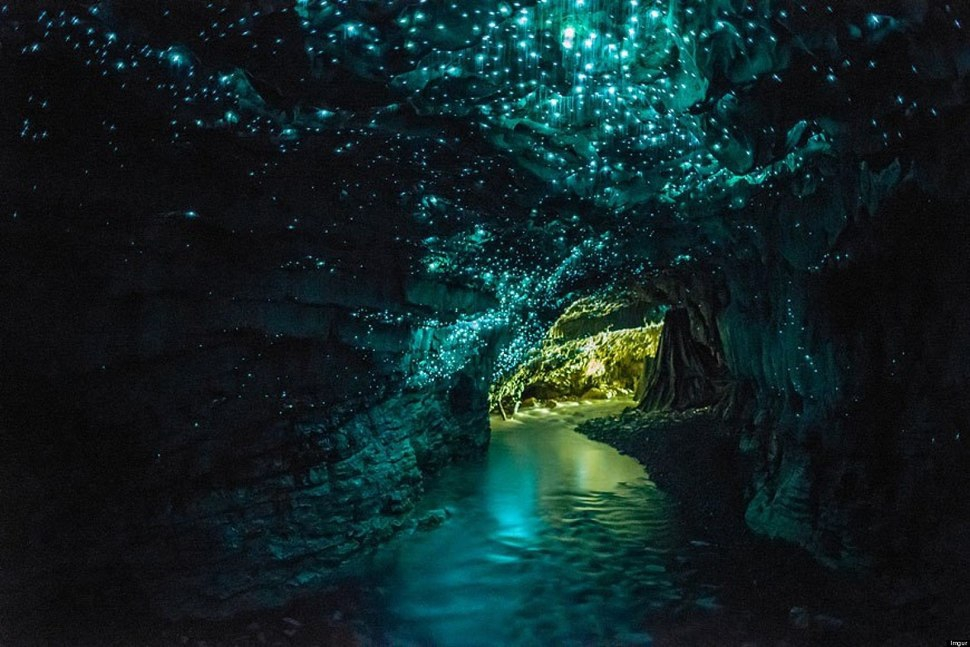
\includegraphics[height=2.8cm,width=1\textwidth,keepaspectratio]{surface_types/splash.png}};
            % Create scope with normalized axes
            \begin{scope}[
                    x={($ 0.1*(image.south east)$)},
                    y={($ 0.1*(image.north west)$)}]
                % Grid and axes' labels
                % \draw[lightgray,step=1] (image.south west) grid (image.north east);
                % \foreach \x in {0,1,...,10} { \node [below] at (\x,0) {\x}; }
                % \foreach \y in {0,1,...,10} { \node [left] at (0,\y) {\y};}
  
                % Labels
                \draw[stealth-, very thick,green] (5,2) -- ++(-2,+1)
                node[rounded corners=3pt,left,black,fill=white]{\tiny Лужа};
            \end{scope}
        \end{tikzpicture}
        \caption{Пещера, заполненная водой по~колено}
        \label{fig:surface_types/splash.png}
    \end{subfigure}
    \hfill
    \begin{subfigure}[b]{0.3\textwidth}
        \centering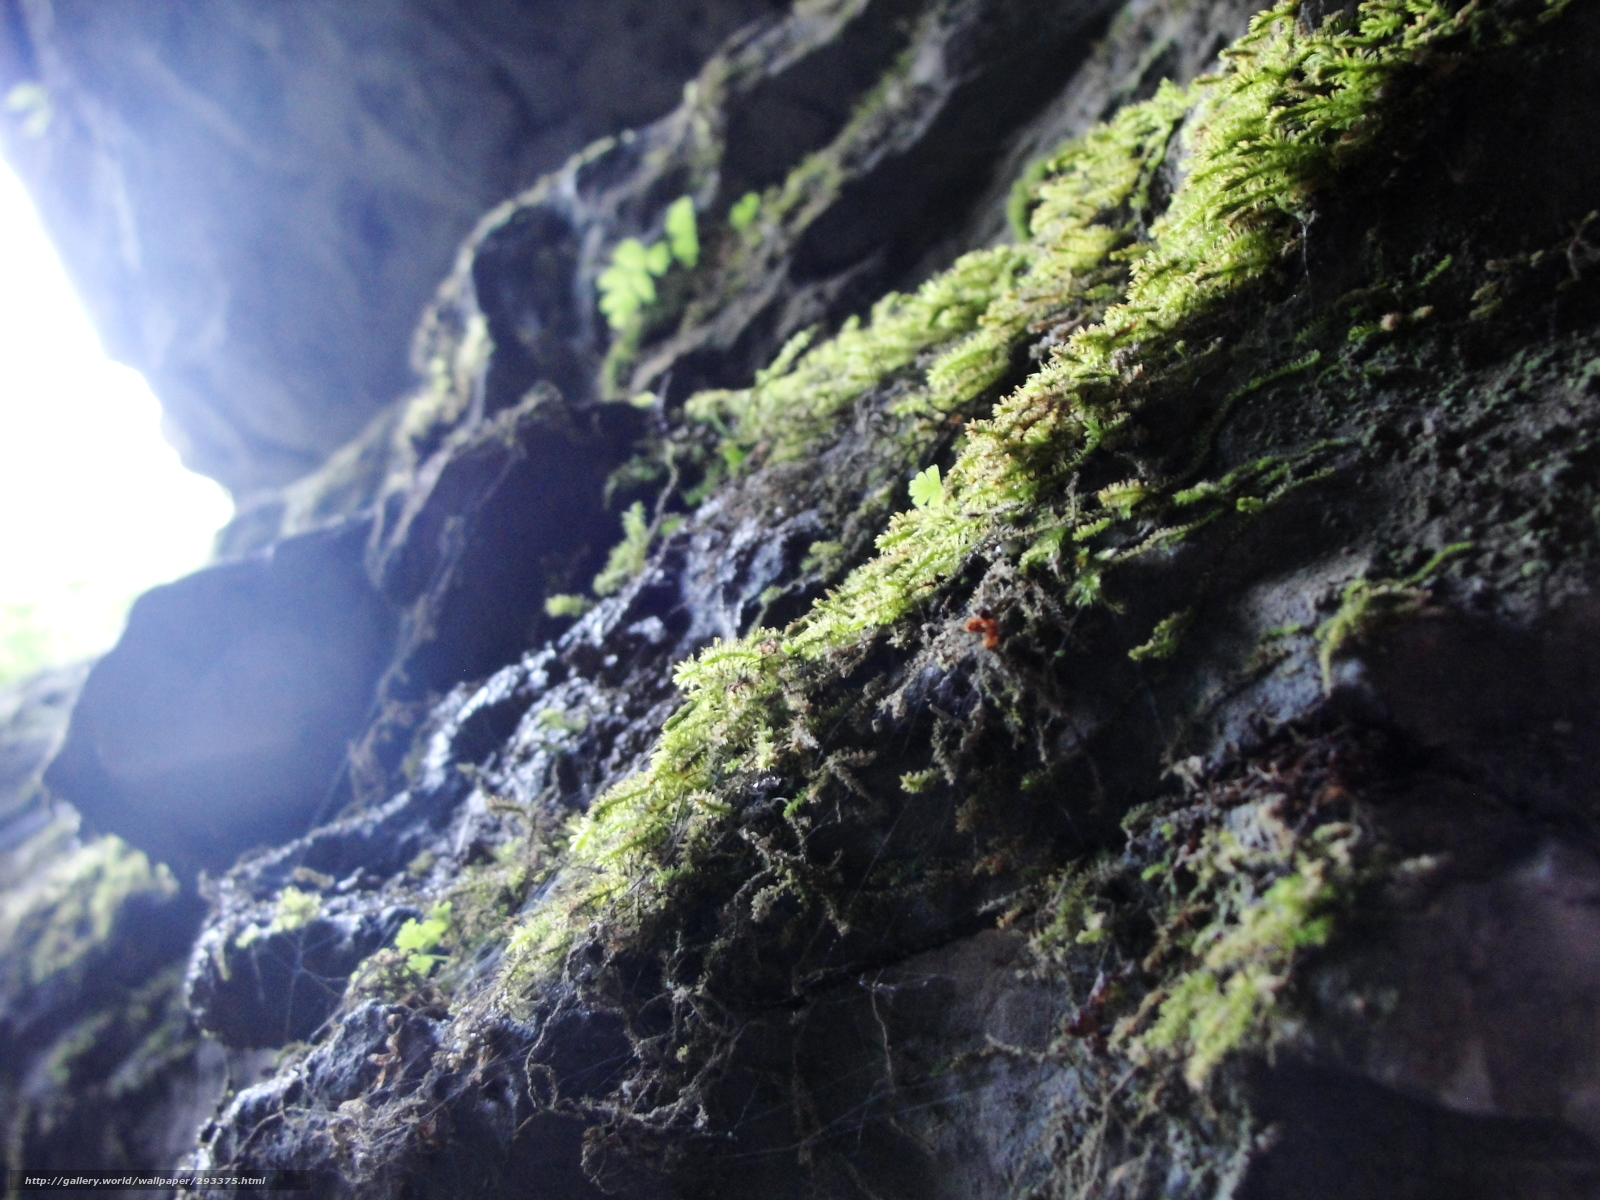
\includegraphics[height=2.8cm,width=1\textwidth,keepaspectratio]{surface_types/moss.jpg}\\
        \caption{Мох}
        \label{fig:surface_types/moss}
    \end{subfigure}
    \caption[Этот текст попадает в названия рисунков в списке рисунков]{Препятствия, встречающиеся в пещерах}\label{fig:obstacles}
  \end{figure}

  Так же были рассмотрены размеры пещер, чтобы понимать необходимый запас хода, размеры робототехнического комплекса. Процентное соотношение суши/воды необходимо понимать, чтобы при разработке робота понимать какой основной функционал необходим.

\subsection{Прототипы роботов}

В диссертации рассматривались различные типы роботов. Те которые создавались специально под пещеры, космические, а так же те, которые потенциально могут быть использованы в условиях, определенных выше.

Как итог, их можно классифицировать следующим образом. Наземные роботы это шагающие, колесные, трековые и необычные. К необычным включены змеевидные, шарообразные и другие.

К летающим были отнесены защищенные дроны и дирижабли.

Но обычно для решения поставленной задачи создается робототехническая система, включающая в себя несколько роботов одного типа или комбинацию наземного и летающего роботов.

\subsection{Методы для получения полезной информации о поверхности}

Под полезной информацией рассматривается как получение самой поверхности, так и получение ее свойств. К примеру тип поверхности.

Были рассмотрены классические SLAM алгоритмы, основанные на использовании камеры, стереопары, с использованием лидара. Так же алгоритмы использующие данные с нескольких сенсоров к примеру с GPS, IMU.

Были найдены способы получения облака точек объекта с помощью касания манипулятором данного объекта. Примерное местоположение объекта определялось камерой.

Определить тип поверхности можно так же с помощью различных сенсоров: визуально, с помощью звука, с помощью датчиков силы и с помощью нескольких сенсоров одновременно.

\subsection{Вывод}
Были найдены следующие предложенные решения:
\begin{itemize}
    \item робототехнические системы для исследования свободных пещер;
    \item Построение карты с помощью лидаров и камер;
    \item Получение конечно элементной сетки с помощью тактильного очувствления манипулятором.
\end{itemize}

Таким образом, поставленная задача является новой и не была решена до этого.

\textbf{\underline{Вторая глава}} покрывает разработку объекта исследования, а именно решение задачи топологического синтеза и инженерную разработку прототипа.

Для эффективного исследования пещер необходимо выставить требования к разрабатываемому роботу. На основании литературного обзора было решено, что робот должен:
\begin{enumerate}
    \item иметь малые габариты, чтобы иметь возможность пролезать через щели в скальной породе и не застревать среди камней;
    \item обладать достаточной проходимостью по сыпучим грунтам;
    \item иметь возможность преодолевать малые водные преграды;
    \item мог взбираться на большие каменные уступы.
\end{enumerate}

Было решено, что цикловой движитель с одной степенью свободы в ноге лучше всего подходит для решения подобных задач.

Для цикловых движителей с одной степенью свободы в ноге вопрос о количестве ног не имеет однозначного решения. Поэтому необходимо провести структурный синтез, чтобы определить их количество. Данная задача решалась с помощью генетического алгоритма.

Генетический алгоритм это эвристический алгоритм поиска, используемый для решения задач оптимизации и моделирования путём случайного подбора, комбинирования и вариации искомых параметров с использованием механизмов, аналогичных естественному отбору в природе. Для решения задачи использовалась библиотека Deap.

Геометрическая модель робота представлена в виде трехмерного параллелепипеда. Количество движителей по каждому из бортов обозначается через $\gamma$. Разность фаз между соседними движителями обозначается через  $\alpha$ \pic{fig:best_gen_robot.jpg}.

\begin{figure}[H]
    \centering
    \begin{tikzpicture}
        % Include the image in a node
        \node [above right, inner sep=0] (image) at (0,0)
        {\centering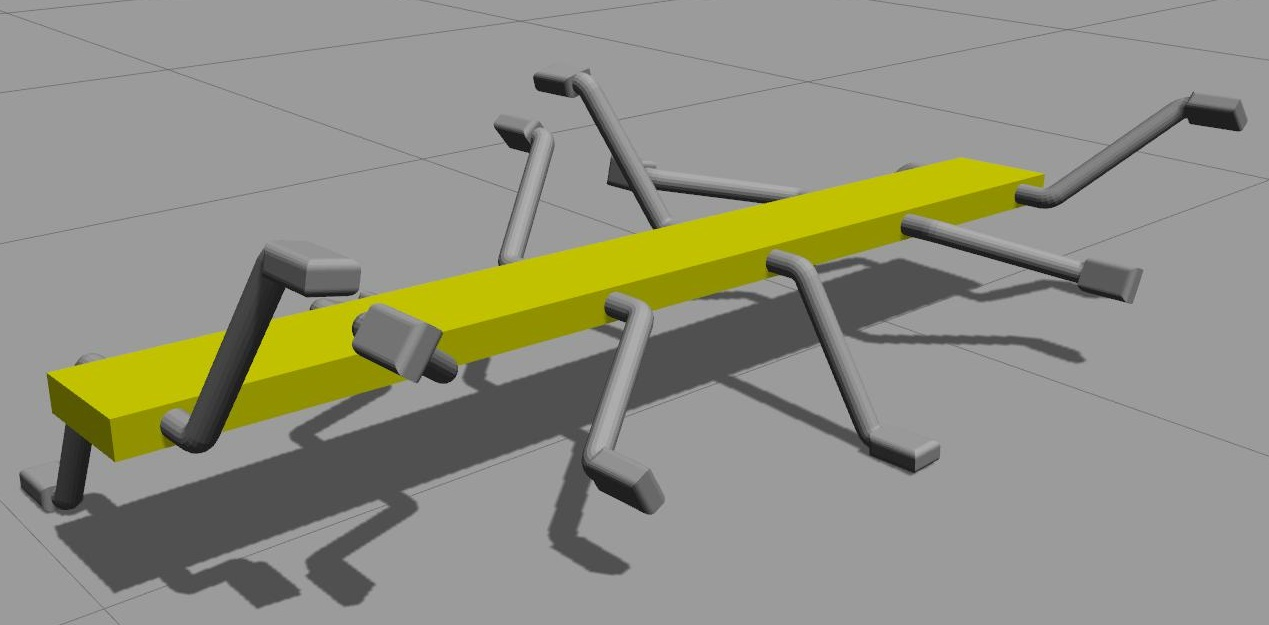
\includegraphics[height=2.7cm,width=1\textwidth,keepaspectratio]{best_gen_robot.jpg}};
        % Create scope with normalized axes
        \begin{scope}[
                x={($ 0.1*(image.south east)$)},
                y={($ 0.1*(image.north west)$)}]
            % Labels
            \draw [green, very thick,
                decorate,
                decoration = {brace,
                        raise=5pt,
                        amplitude=5pt,
                        aspect=0.5}] (1.4,3.6) --  (8.1,6.8)
            node[rounded corners=3pt, pos=0.5,above left =14pt,black,fill=white]{\tiny $(\gamma - 1) h_{\text{leg}}sin(\alpha)$};

            \draw[stealth-, very thick,green] (9.5,7.8) -- (7.8,1.94);
            \draw[stealth-, very thick,green] (1.5,2.8) -- (7,1)
            node[rounded corners=3pt,right,black,fill=white]{\tiny $\gamma = 6$};

            \draw[thin,green] (6.7,4) -- (5.75,9);
            \draw[thin,green] (4.85,3.5) -- (5.75,9);
            \draw[thin,green,stealth-stealth] (6.32,6) arc (-79.2:-99.2:3) node [rounded corners=3pt,below = 2pt,black,fill=white, midway] {\tiny $\alpha$};
        \end{scope}
    \end{tikzpicture}
    \caption{Схема модели робота для генетического алгоритма}
    \label{fig:best_gen_robot.jpg}
\end{figure}

Эту задачу можно сформулировать как мультикритериальную задачу оптимизации, где необходимо максимизировать дистанцию, пройденную за фиксированное время, и минимизировать длину робота \eqref{eq:second}. Параметрами индивида являлись $\gamma$ и $\alpha$.

\begin{eqnarray}
    \label{eq:second}
    F \rightarrow max = \beta \left( {\omega}_{1} \cdot \overbrace{\delta}^{\text{Distance}} + {\omega}_{2} \cdot \overbrace{\frac{1}{(\gamma - 1) h_{\text{leg}}sin(\alpha)}}^{\text{Simplified body length}}\right) + \\ \nonumber + (1 - \beta) {\delta}^{{\omega}_{1}} {\left( \frac{1}{(\gamma - 1)h_{\text{leg}}sin(\alpha)}\right)}^{{\omega}_{2}}
\end{eqnarray}
где $\delta$ дистанция, $\beta$ адаптивный параметр, ${\omega}_{1,2} \in  [ 0..1 ] $ весовые коэффициенты.


Весовые коэффициенты настраивались в зависимости от выбора приоритета. Невзирая на выбранные коэффициенты, оптимальным набор ног начинался с 8 и заканчивался 14. Это объясняется критерием статического равновесия, который, как оказалось, увеличивает проходимость механизма. В данном случае 4 ноги всегда будут касаться пола. 

Было проведено два испытания. На первом испытании мы стремились найти только одного лучшего робота, только для местности T1 \pic{fig:terrain_1}. На втором этапе мы хотели видеть зависимость от разных типов ландшафтов при меньшем количестве индивидуальностей.

Первый этап: каждый робот проходил 10 разных ландшафтов по 9 секунд каждую. Вторая фаза: она имеет те же параметры, что и первая фаза, но с измененным размером популяции. 

В соответствии с таблицей \ref{tabular:Table2} (весовые коэффициенты равны 0.6 и 0.4 соответственно) видно, что мы имеем сходимость в параметрах. Видео прохождения препятствия лучшим индивидом \quad
\qrcode[height=1.5cm]{https://youtu.be/DcovvkTZgsg}

\begin{figure}[h]
    \begin{subfigure}{0.33\textwidth}
    \centering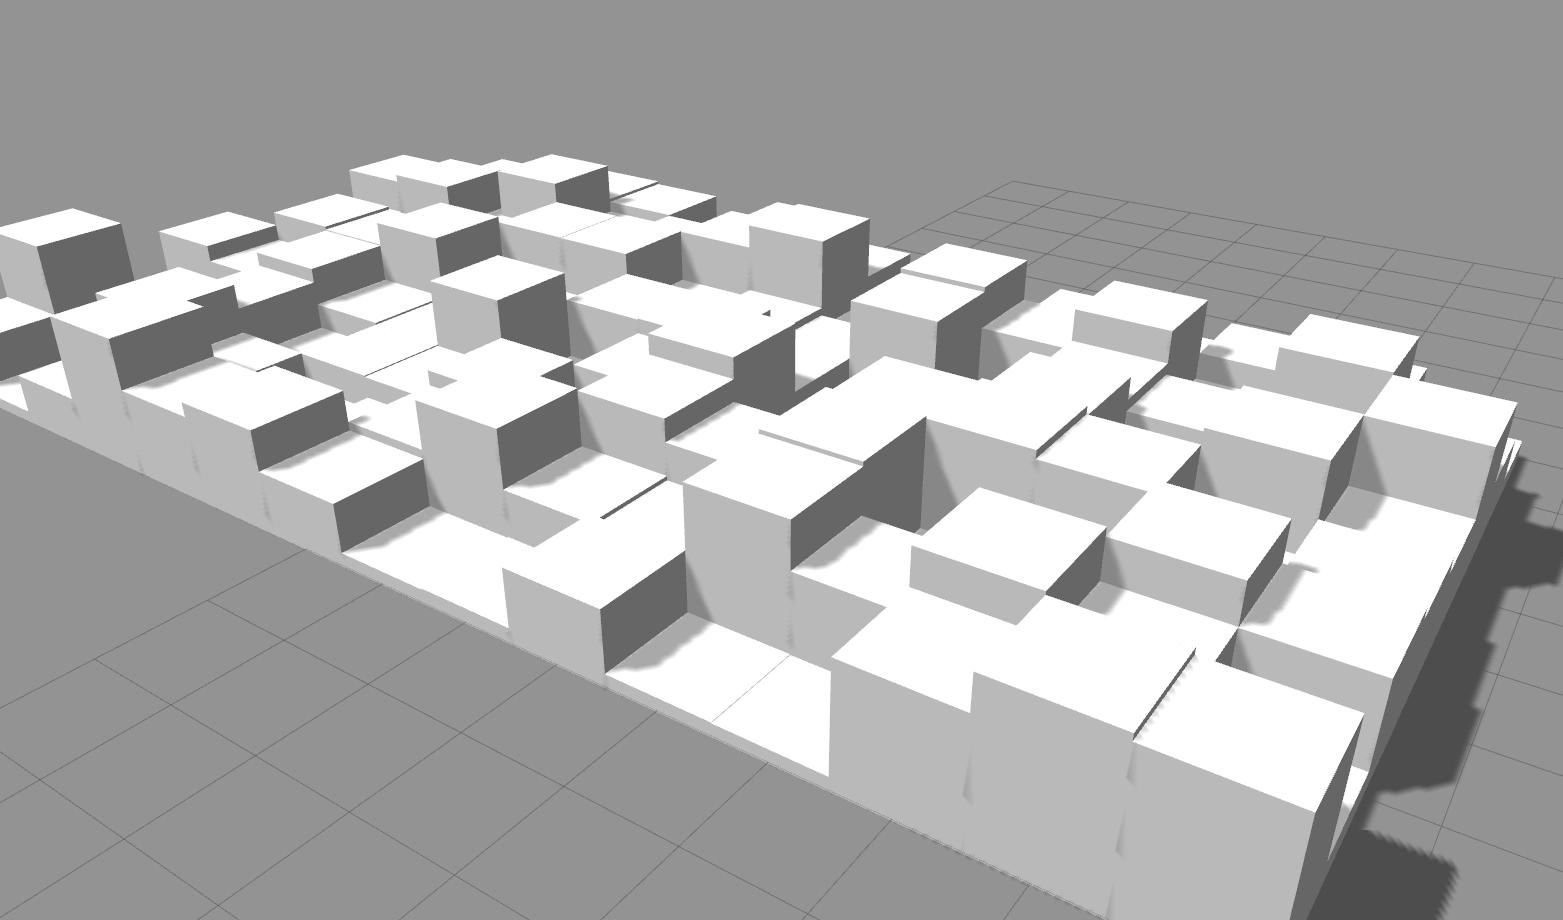
\includegraphics[width=0.8\textwidth]{terrain_1} 
    \caption{T1: 3D-боксы с равномерным распределением высоты}
    \label{fig:terrain_1}
    \end{subfigure}
    \begin{subfigure}{0.33\textwidth}
    \centering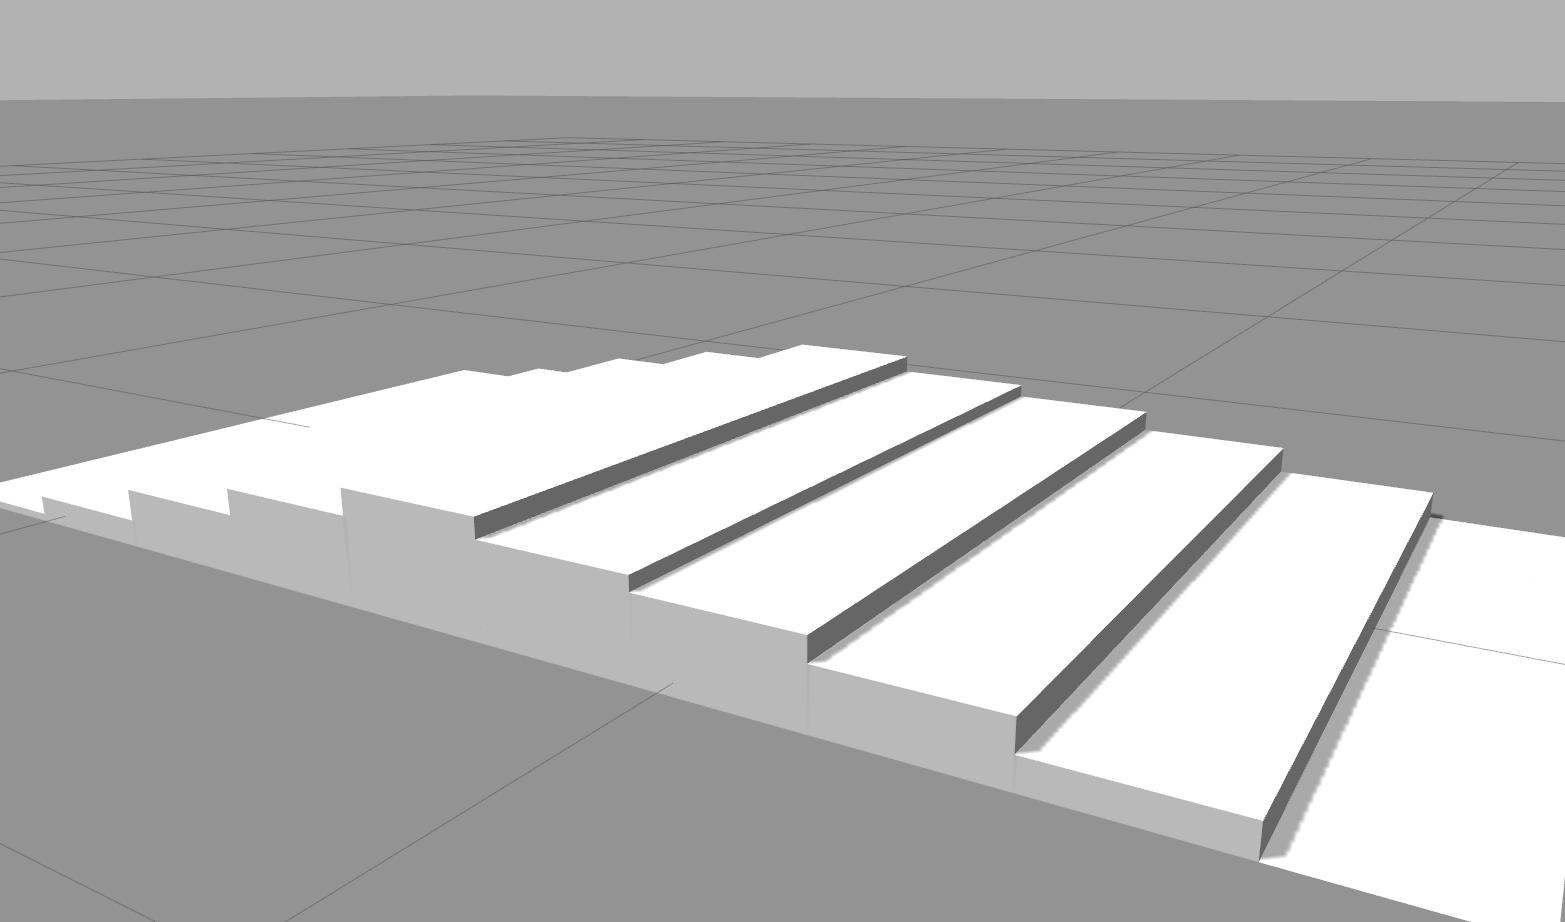
\includegraphics[width=0.8\textwidth]{terrain_2} 
    \caption{T2: 2D-полосы с гауссовой функциональной высотой}
    \label{fig:terrain_2}
    \end{subfigure}
    \begin{subfigure}{0.33\textwidth}
    \centering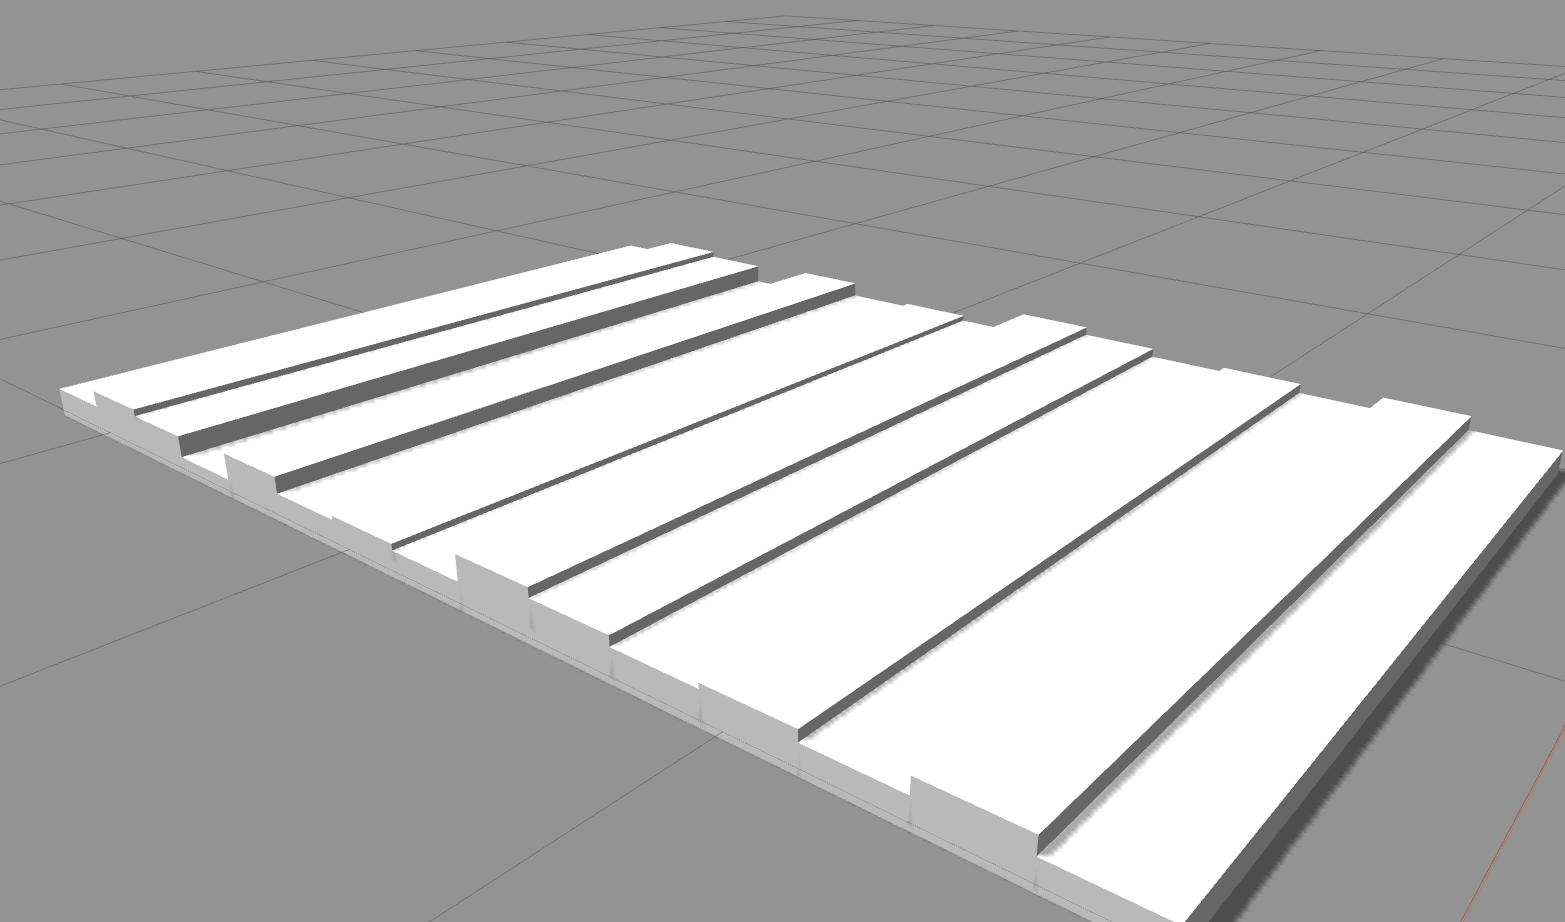
\includegraphics[width=0.8\textwidth]{terrain_3}
    \caption{T3: 2D-полосы с распределением высоты по гауссовской функции)}
    \label{fig:terrain_3}
    \end{subfigure}
     
    \caption{Примеры сгенерированных территорий}
    \label{fig:terrains}
\end{figure}
\vspace{-0.5cm}

\begin{table}[H]
\caption{Зависимость между статистикой значения пригодности и типами ландшафта}
\label{tabular:Table2}
\begin{center}
\begin{tabular}{c|c|c|c}

\textbf{\makecell{Территория, популяция}} & \textbf{\makecell{Параметры}} & \textbf{\makecell{Среднее \\значение }} & \textbf{\makecell{Std \\целевая функция}}\\
\hline
\textbf{\makecell{T1 \pic{fig:terrain_1}, 110}} & \makecell{(6, 72)} & \makecell{2.38} & \makecell{0.34}
\\
\textbf{\makecell{T2 \pic{fig:terrain_2}, 55}}& \makecell{(5, 68)} & \makecell{1.95} & \makecell{0.35} 
\\
\textbf{\makecell{T3 \pic{fig:terrain_3}, 55}} & \makecell{(6, 77)} &  \makecell{2.08} & \makecell{0.33} \\
\hline
\end{tabular}
\end{center}
\end{table}

В первом пункте требований к движителю (начало главы) стоит требование, чтобы робот не застревал при поворотах. Проблема застревания решается с помощью изменения угла между ногой и корпусом робота.

\begin{figure}[H]
    \centering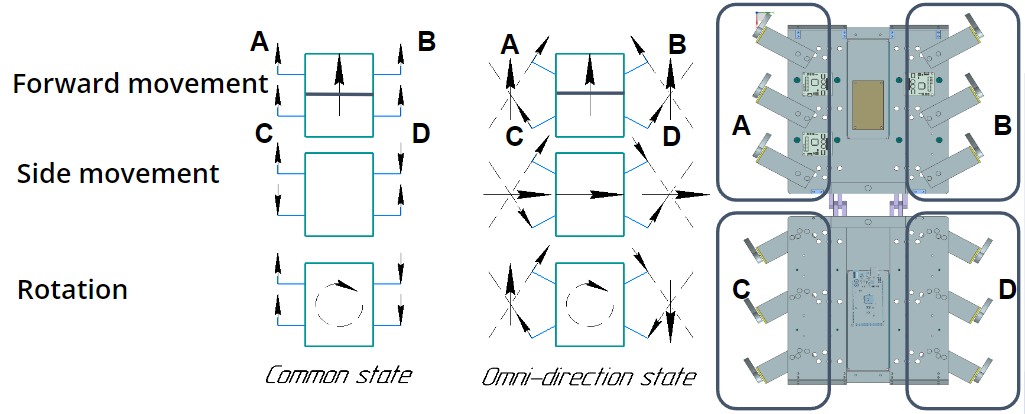
\includegraphics[height=3cm,width=1\textwidth,keepaspectratio]{omni_rot.png}
    \caption{Векторное представление сил в классическом и всенаправленном состоянии}
    \label{fig:omnidirection}
\end{figure}

На рисунке \ref{fig:omnidirection} представлена иллюстрация данной концепции: для того, чтобы робот двигался во всех направлениях, необходимо разбить ноги на группы, чтобы получилось 4 группы A-D.

Если сравнивать с классической компоновкой роботов (угол между корпусом робота и осью вала привода ноги равен 90 градусов), то вектор внешних сил будет таким, как на левой части рис. \ref{fig:omnidirection}. Стрелка в центре робота — суперпозиция всех сил. Если изменить угол оси привода ноги в соответствии с предлагаемой концепцией, то возможно получить значения суперпозиции сил, представленные на рис. \ref{fig:omnidirection} в центре. То есть, чтобы переместить корпус робота направо, группы А и D должны вращать ноги в одну сторону, а группы C и B — в противоположную. Правая часть рисунка иллюстрирует расположение групп ног на исследуемом роботе. 

В рамках исследования было разработано четыре концепции робота СтриРус. В таблице \ref{tabular:robot_comparison} в строке недостатки объясняются основные причины перехода из одной итерации к другой. Концептуально было замечено, что высота ноги и наличие сегмента разительно влияет на проходимость конструкции. \quad \qrcode[height=1.5cm]{https://youtu.be/EQ6oGZVDpoc}

\begin{figure}[H]
    \centerfloat{
        \hfill
        \subcaptionbox[List-of-Figures entry]{Первая итерация\label{fig:strirus_0}}{%
            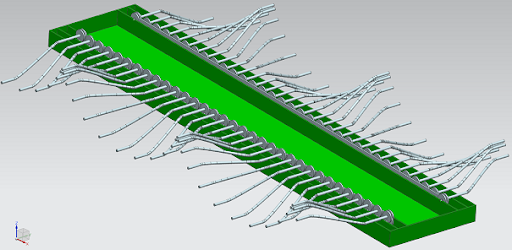
\includegraphics[width=0.33\linewidth]{strirus_0.png}}
        \hfill
        \subcaptionbox[List-of-Figures entry]{Вторая итерация \label{fig:strirus_1}}{%
            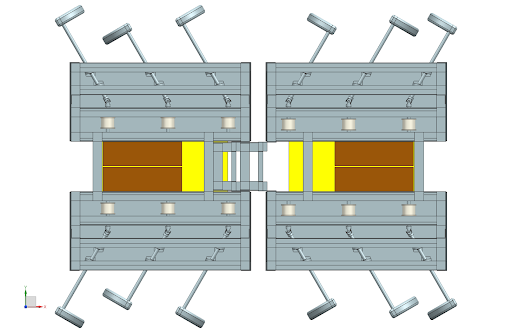
\includegraphics[width=0.33\linewidth]{strirus_1.png}}
        \hfill
        \subcaptionbox{Третья итерация\label{fig:strirus_2}}{%
        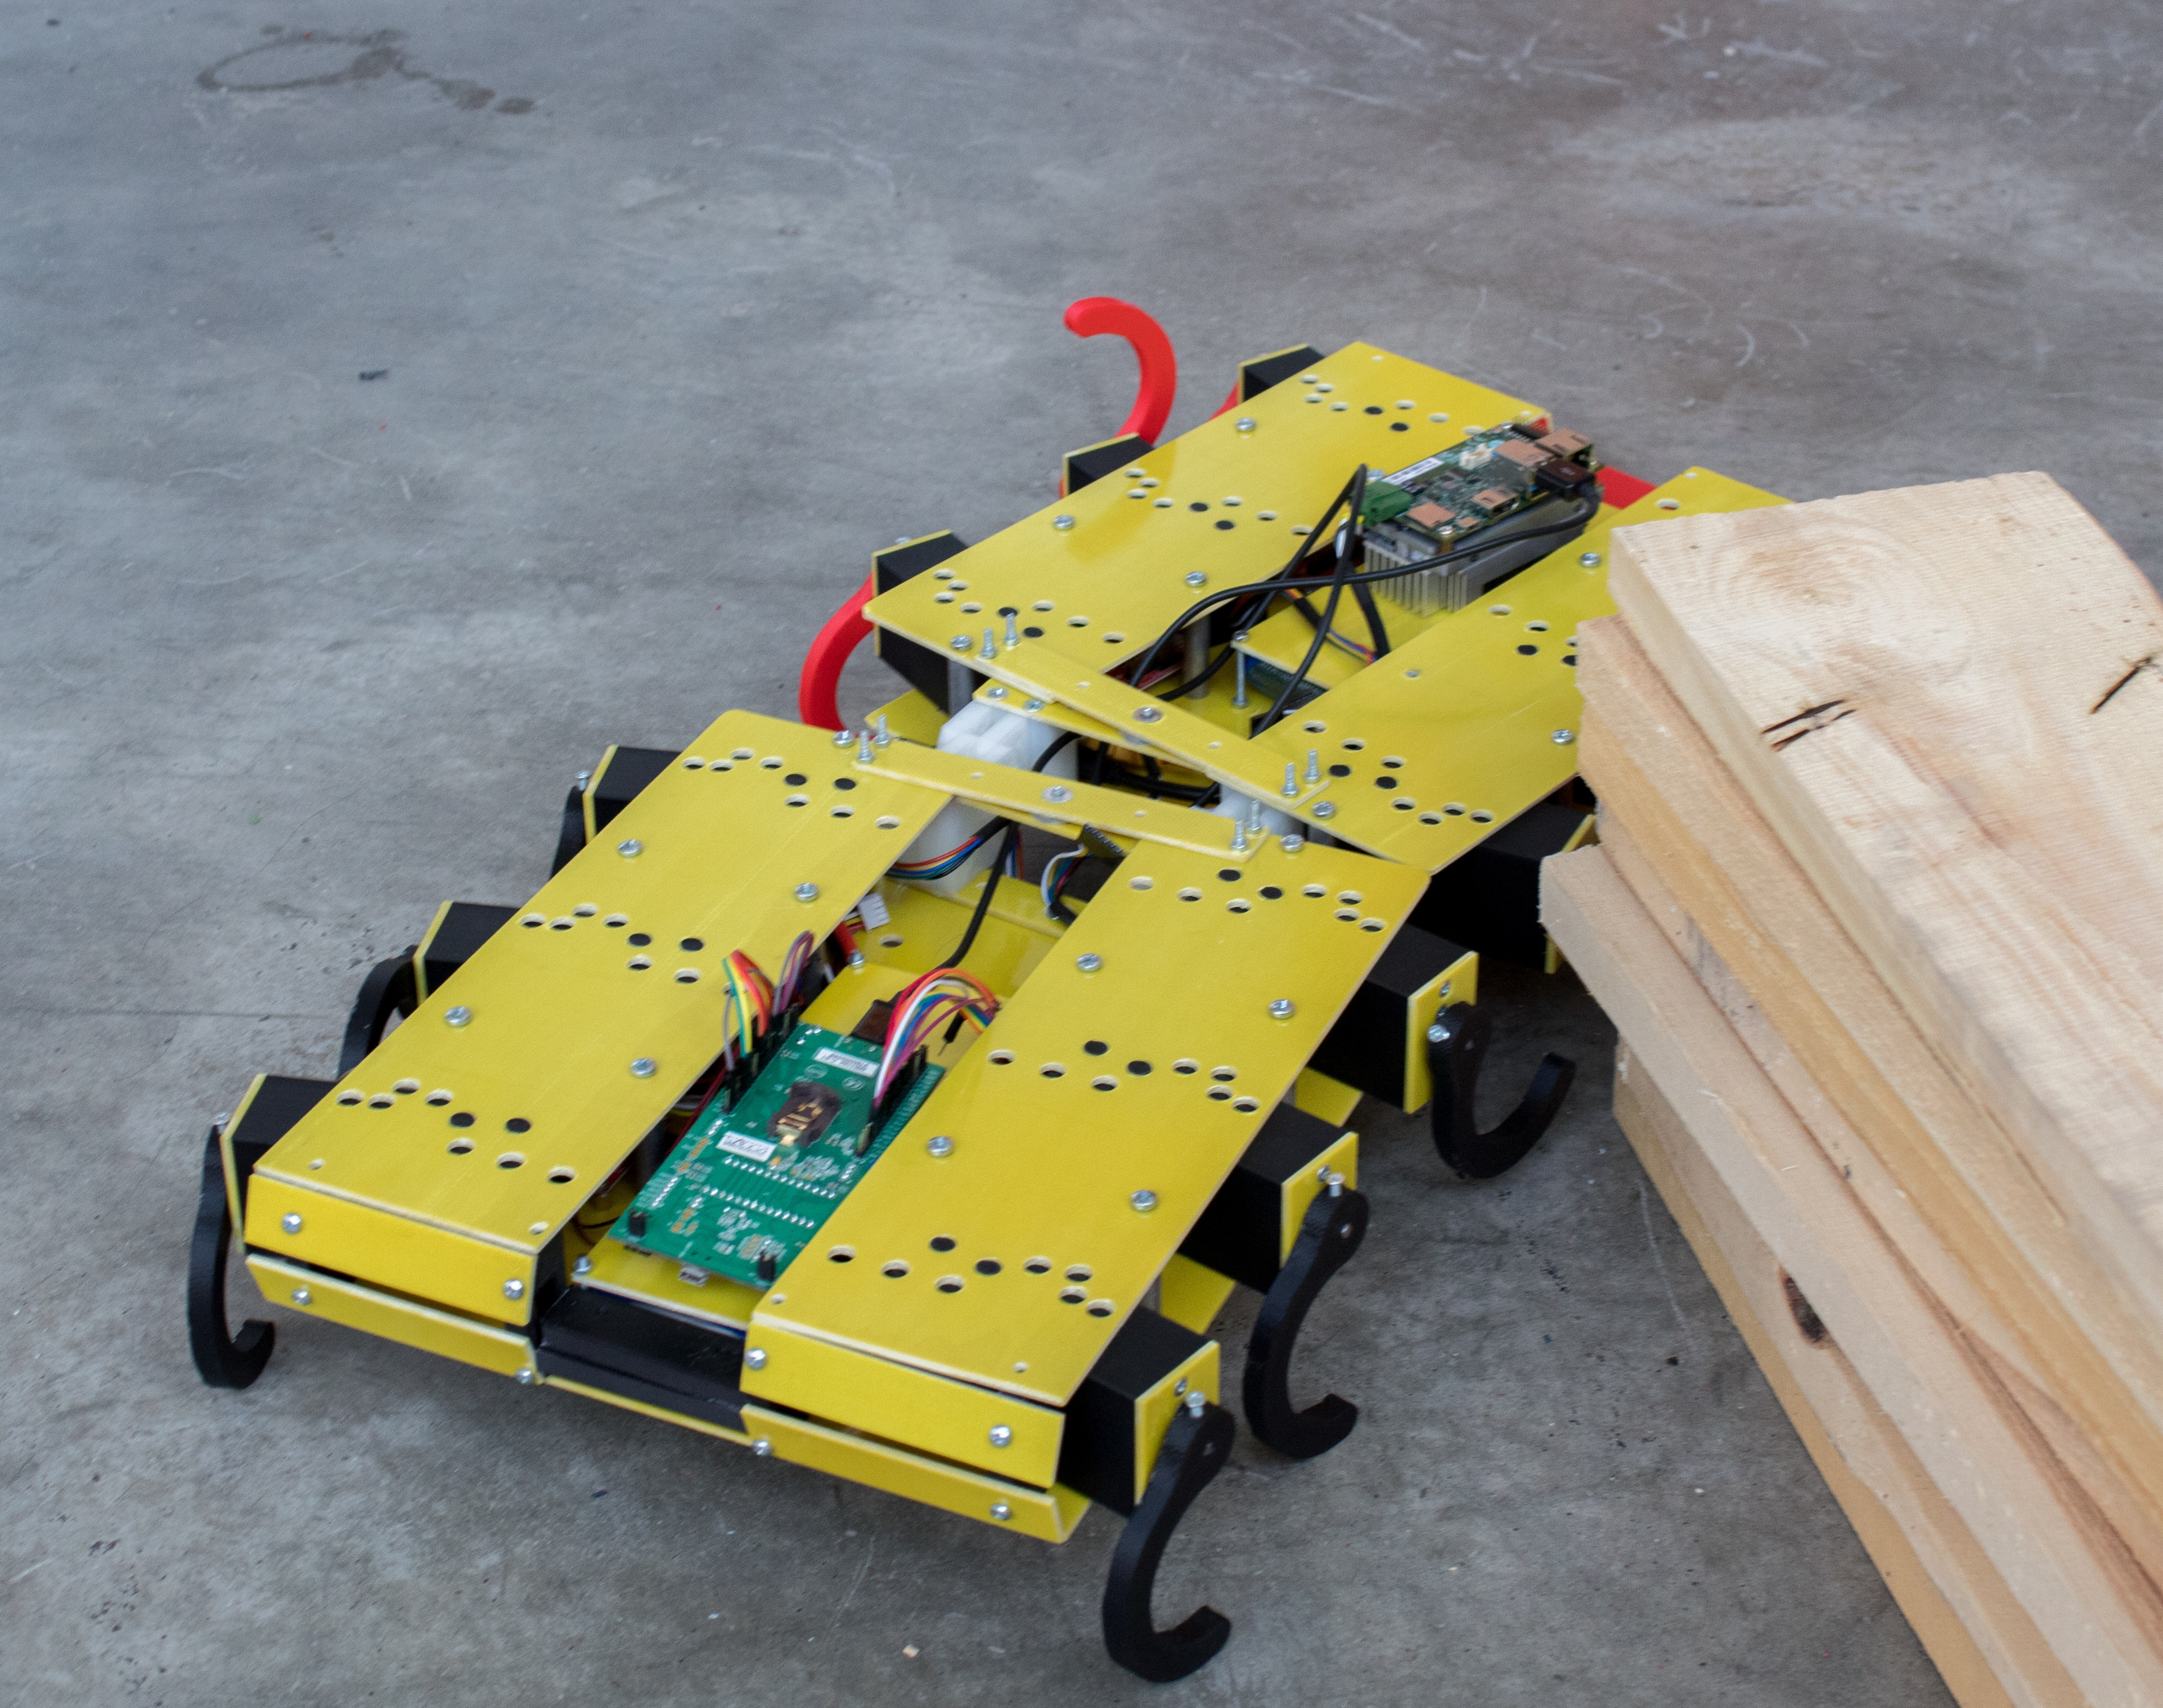
\includegraphics[width=0.33\linewidth]{strirus_2.jpg}}
        \hfill
        \subcaptionbox{Третья итерация, улучшенная\label{fig:strirus_3}}{%
        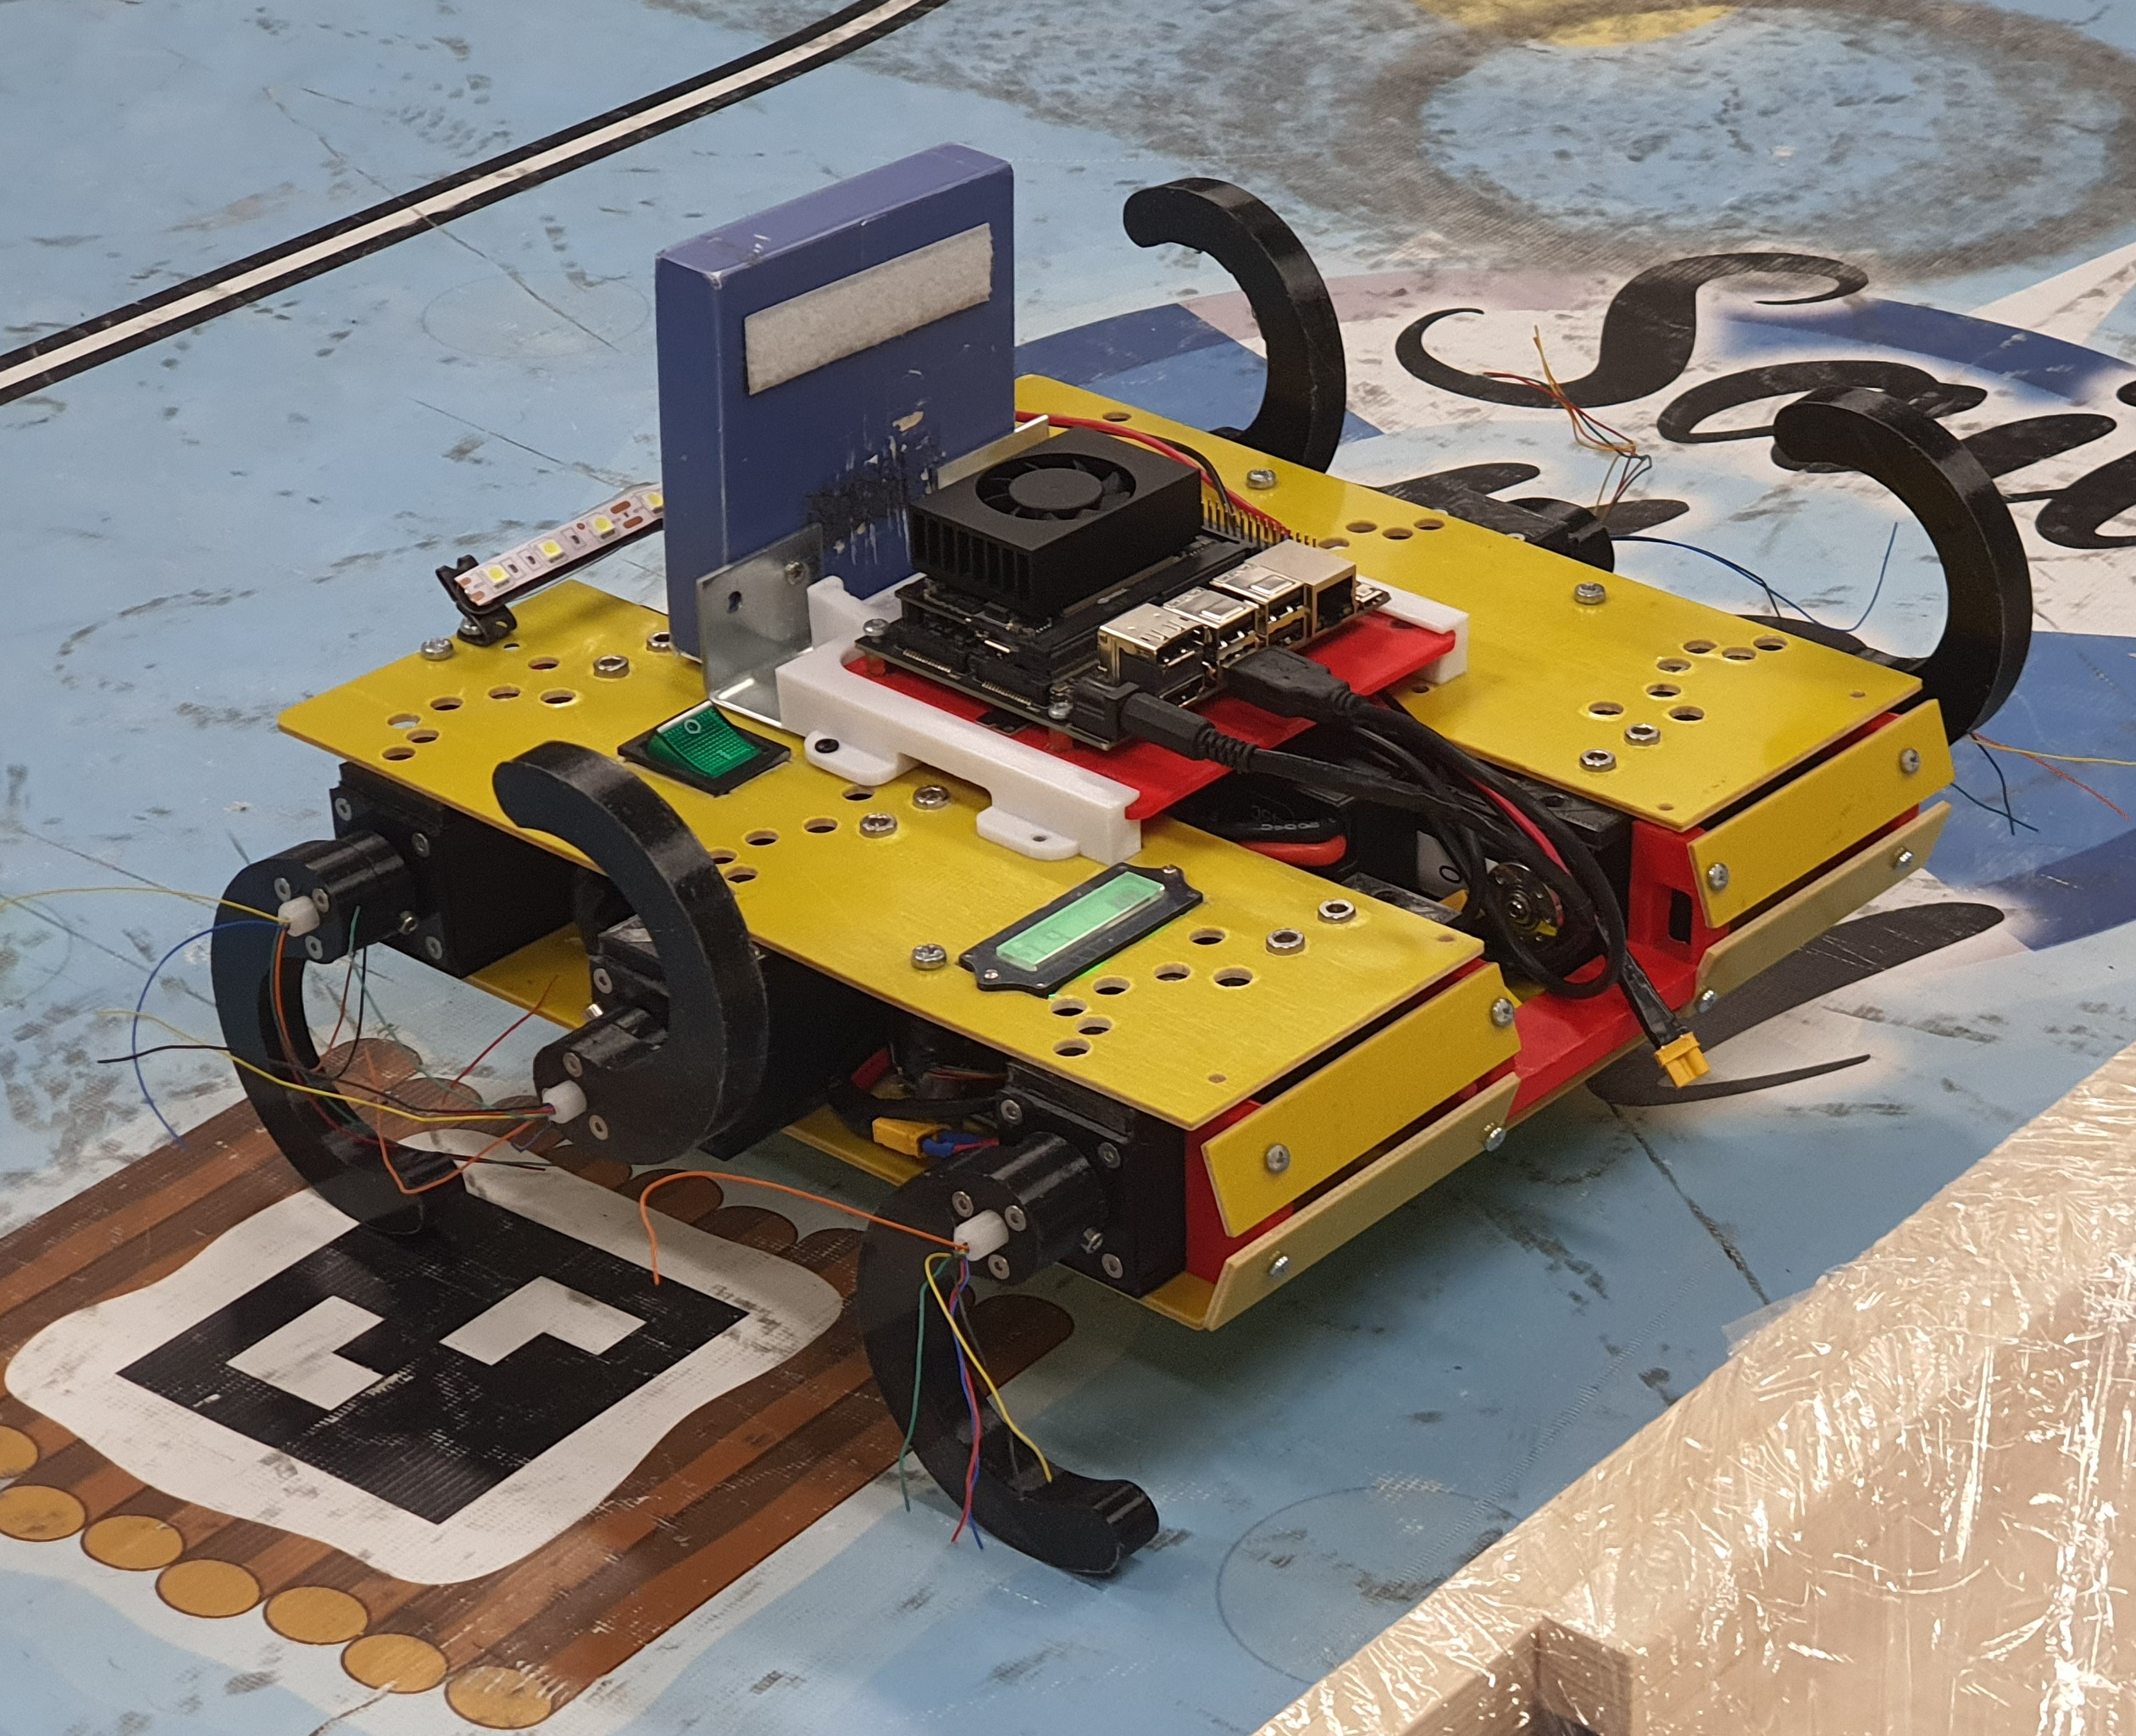
\includegraphics[width=0.35\linewidth]{strirus_3.JPG}}
        \hfill
        \subcaptionbox{Четвертая итерация\label{fig:strirus_4}}{%
        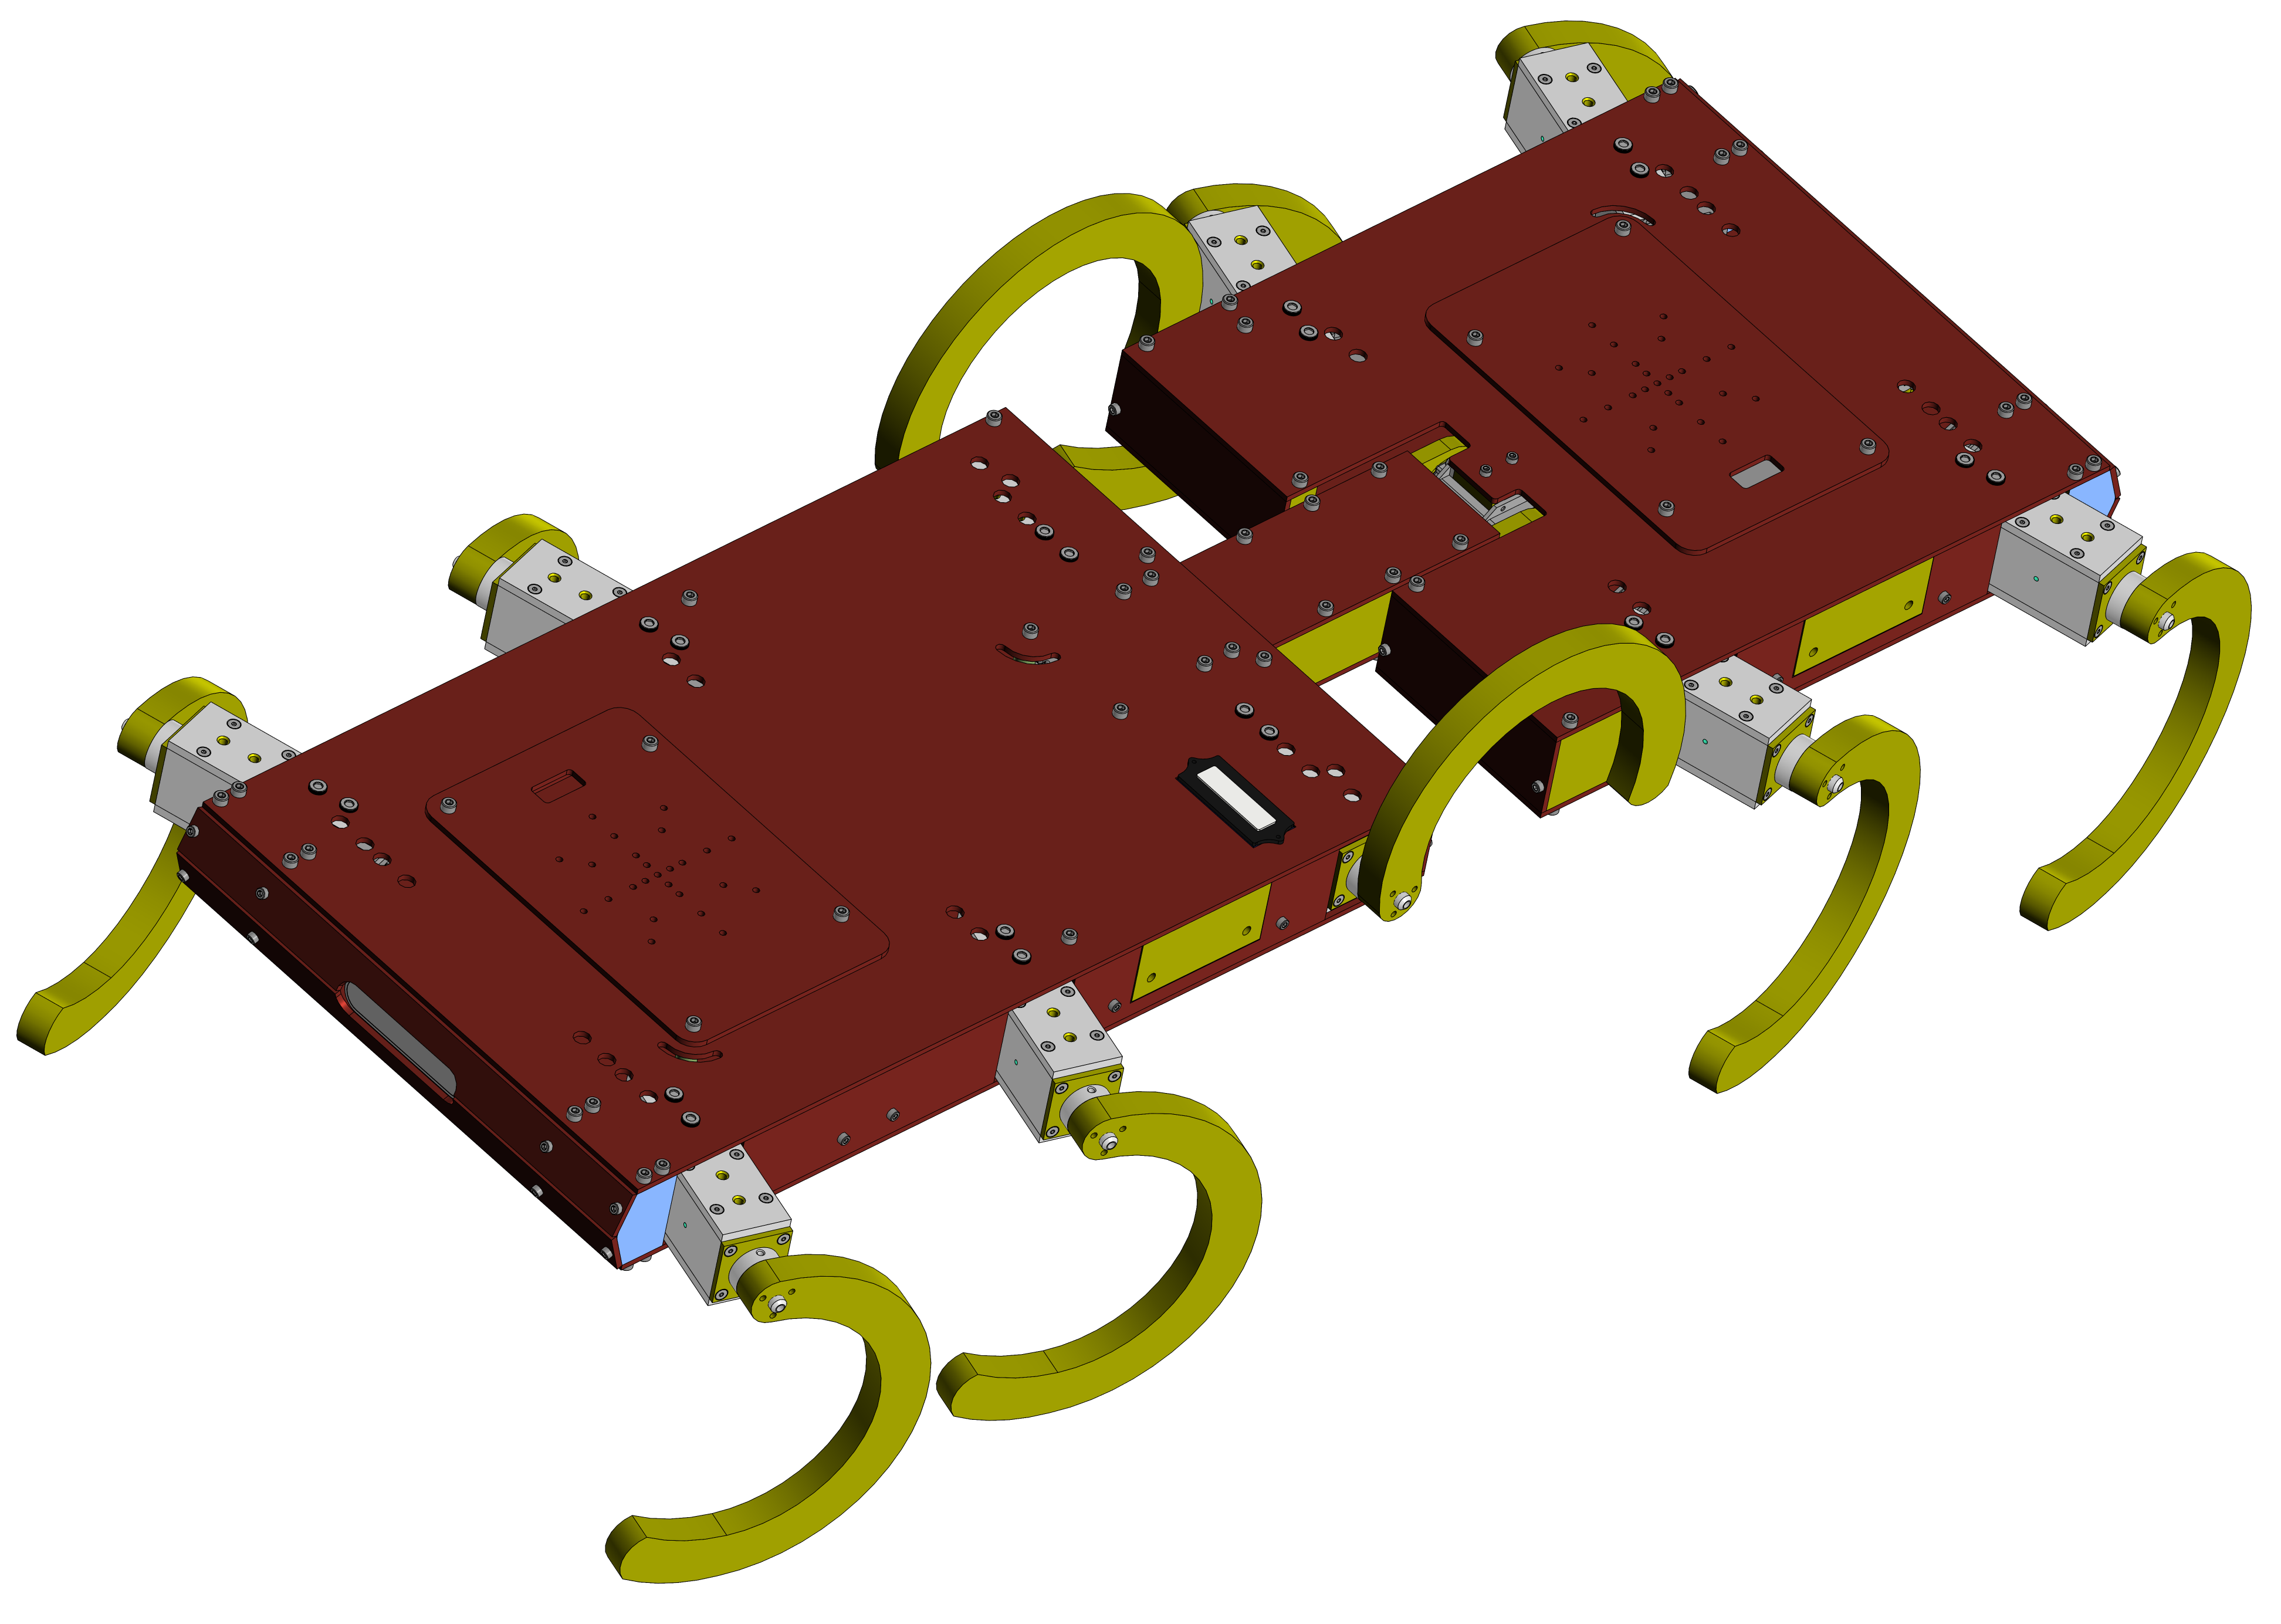
\includegraphics[width=0.35\linewidth]{strirus_4.png}}
    }
    % \legend{Подрисуночный текст, описывающий обозначения, например. Согласно
    %     ГОСТ 2.105, пункт 4.3.1, располагается перед наименованием рисунка.}
    \caption{Итерации робота СтриРуса}\label{fig:striruses}
  \end{figure}

\vspace{-1cm}

\begin{table}[H]
    \caption{Сравнение итераций робота}
    \label{tabular:robot_comparison}
    % \begin{center}
    \begin{footnotesize}
    \begin{tabular}{p{1.6cm}|p{1.6cm}|p{1.5cm}|p{1.7cm}|p{1.4cm}|p{1.4cm}}
    \toprule
    \toprule
    % \rowcolor{Gray}
     Итерация & 1 \pic{fig:strirus_0}  & 2 \pic{fig:strirus_1} &  3 \pic{fig:strirus_2} & 3+ \pic{fig:strirus_3} & 4 \pic{fig:strirus_4} \\
     \hline
     Кол-во ног & 54 & 12 & 12 & 6 & 10 \\ 
    %   \rowcolor{lightgray}
     \makecell[l]{Кол-во \\ сегментов} & 1 & 2 & 2 & 1 & 2 \\
     \makecell[l]{Тип \\ соединения} & --- & Тангаж & \makecell[l]{Тангаж,\\ рыскание} & --- & Тангаж \\
    %  \rowcolor{lightgray}
     Отн. угол телом -- нога, градусы & 0 & 0--45 & 0, 15, 30, 45 & 0 & 0, 15 \\
     \makecell[l]{Высота \\ ноги, мм} & 54 & 60 & 60 & 90 & 170 \\
     \hline
     Особенности & Волноход & Механизм, который позволяет непрерывно изменять отн. угол & Двухстепенной узел, соединяющий сегменты & Большие ноги & Гигантские ноги  \\
    %  \rowcolor{lightgray}
    \hline
     Недостатки & Невозможно установить сенсоры на ноги. Много подвижных частей & Слишком сложный механизм, изменяющий отн. угол & Мал. ноги. Избыточная вторая степень свободы в соединительном узле & 1 сегмент. Маленькие ноги & --- \\
    \bottomrule
    \bottomrule
    \end{tabular}
    \end{footnotesize}
    % \end{center}
    \end{table}

Как итог, был разработан 10 ногий двух сегментный робот СтриРус. 10 ног было выбрано на основе результатов, полученных во время решения мультикритериальной задачи оптимизации с помощью генетического алгоритма.

Конструкция робота соответствует всем требованиям, поставленным вначале. А именно, возможность проходить сквозь узкие пространства, иметь возможность преодолевать большие каменные гряды и возможность эффективно перемещаться по сыпучим грунтам.



Существует несколько типов датчиков, которые могут измерять контактные силы и распределение давления. Это могут быть оптические, пьезорезистивные, пьезоэлектрические, магнитные, емкостные, на основе оптических волокон. Промышленные датчики силы и момента (F/T) широко распространены на гуманоидах (Atlas, Fedor) или четвероногих (Spot, AnyMal). Однако они слишком велики для небольших роботов, таких как RHEX, WHEGS или StriRus.

Та же проблема применима к оптическим и магнитным датчикам. Емкостные датчики требуют высокой точности изготовления. Кроме того, датчики перечисленных типов довольно дороги, что делает их использование нецелесообразным в исследовательских роботах, которые работают в опасных условиях и могут быть потеряны в процессе исследования пещеры. Недорогой альтернативой являются тензометрические датчики.

Самый популярный тип тензометрического датчика -- тензорезистивный датчик. Другой тип -- пьезорезистивные датчики на основе проводящих волокон или полимеров. Они недорогие, очень гибкие и компактные. Одним из основных недостатков является значительный гистерезис. В представленной работе используется материал Velostat (Linqstat) \pic{fig:velostat_sensor.jpg} в качестве промежуточного слоя для датчика \pic{fig:simplest_sensor.jpg}.

\begin{figure}[h]
    \begin{subfigure}[t]{0.45\textwidth}
        \centering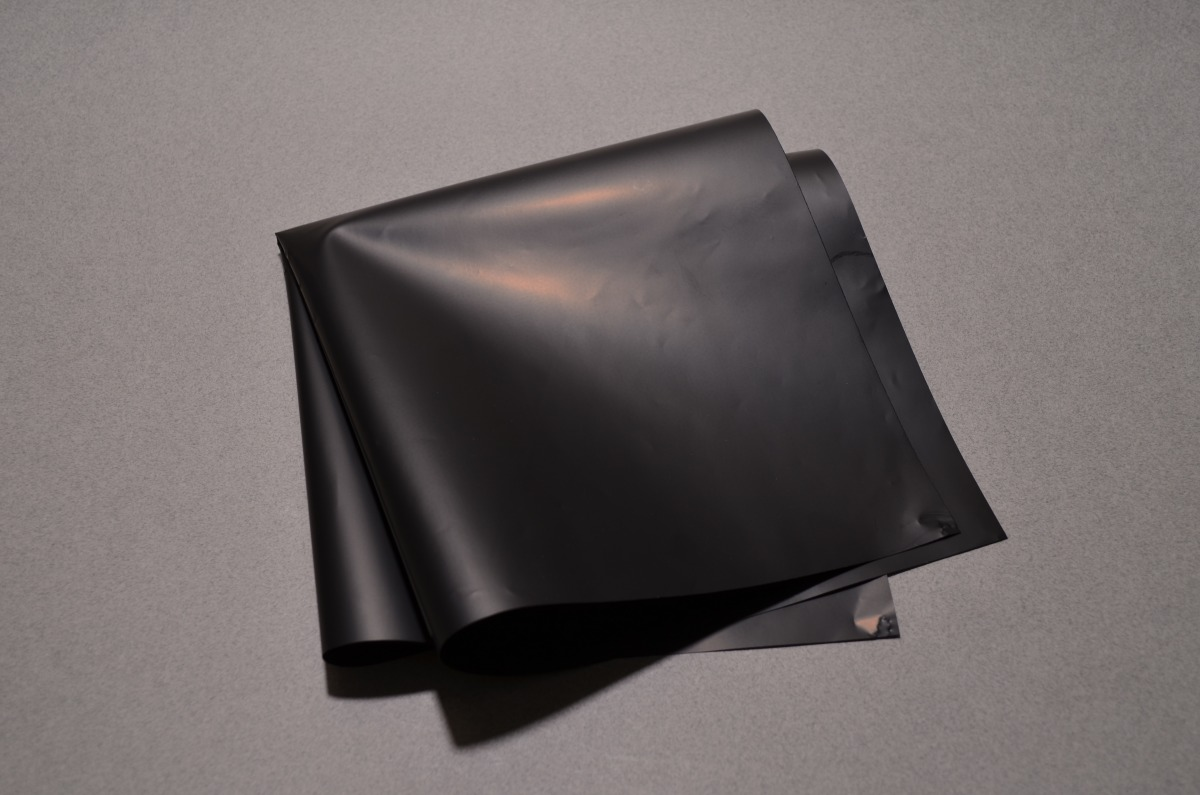
\includegraphics[height=2.5cm,width=1\textwidth,keepaspectratio]{velostat_sensor.jpg}
        \caption{Материал Velostat}
        \label{fig:velostat_sensor.jpg}
    \end{subfigure}
    \begin{subfigure}[t]{0.45\textwidth}
        \centering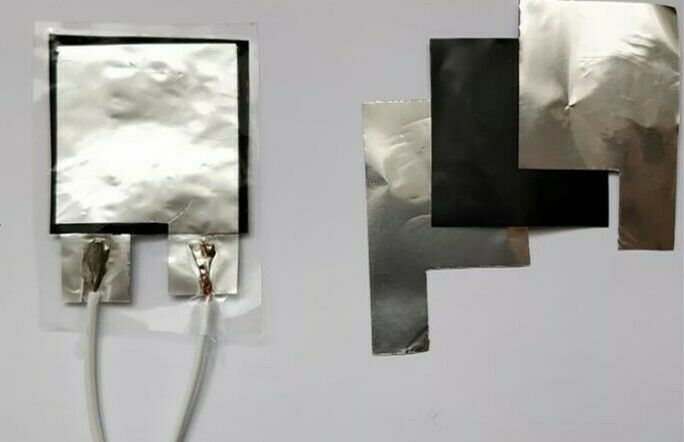
\includegraphics[height=2.5cm,width=1\textwidth,keepaspectratio]{simplest_sensor.jpg}
        \caption{Простейший преобразователь силы на основе Velostat}
        \label{fig:simplest_sensor.jpg}
    \end{subfigure}
    \caption{Примеры использования Velostat}
\end{figure}

При исследовании преобразователя силы на основе Velostat, было замечено, что площадь нажатия разительно влияет на показания преобразователя. Площадь контакта может сильно повлиять на данные при перемещении роботом по неровной твердой поверхности, к примеру по камням. Поэтому было решено характеризовать материал для случаев, когда нагрузка меньше, чем размер сенсора.

Созданный преобразователь состоит из двух медных оболочек, разделенных слоем Velostat. Давление на датчик приводит к изменению его сопротивления: чем выше давление, тем ниже сопротивление. На \pic{fig:velostat_pressure_resistance.jpg} показана рабочая область сенсора, основанная на весе, который может быть приложен на одну лапку робота.
\begin{figure}[h]
    \centering
    \begin{tikzpicture}
        % Include the image in a node
        \node [above right, inner sep=0] (image) at (0,0)
        {\centering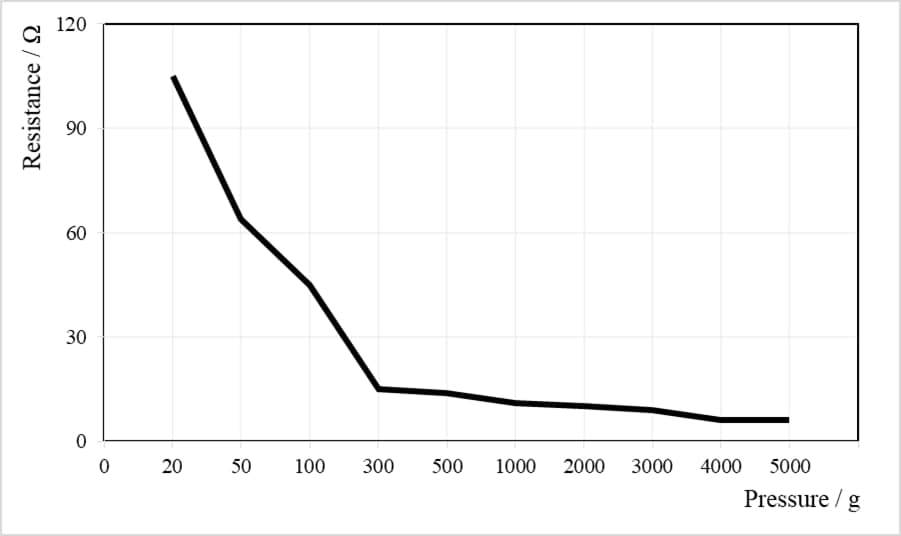
\includegraphics[height=3.5cm,width=1\textwidth,keepaspectratio]{velostat_pressure_resistance.jpg}};
        % Create scope with normalized axes
        \begin{scope}[
                x={($ 0.1*(image.south east)$)},
                y={($ 0.1*(image.north west)$)}]
            \draw[stealth-, very thick,green] (4.21,2.75) -- (6.5,5);
            \draw[stealth-, very thick,green] (8.75,2.15) -- (6.5,5)
            node[rounded corners=3pt,above,black,fill=white]{\small Рабочая область};
        \end{scope}
    \end{tikzpicture}
    \caption{График зависимости прикладываемого веса от сопротивления}
    \label{fig:velostat_pressure_resistance.jpg}
\end{figure}

\subsubsection{Экспериментальный
    стенд}

Для исследования преобразователя Velostat, когда нагрузка меньше, чем размер преобразователя, необходимо сделать лабораторный стенд. Среди требований к стенду можно отметить: необходимость контролировать силу нажатия и повторяемость эксперимента как по величине, так и по расположению площадки контакта инструмента и исследуемого преобразователя силы. Указанным требованиям возможно удовлетворить, используя коллаборативный робот-манипулятор, который будет управляться с помощью impedance управления.

Использование коллаборативного робота позволяет также удовлетворить требованиям безопасности и допустить работу робота в непосредственно близости от экспериментатора. Разработанный стенд, представлен на рисунке \ref{fig:exp_standd}. \href{https://youtu.be/Gw4wVZ-ESuE}{Видео работы стенда}.

\begin{figure}[h]
    \begin{center}
        \begin{subfigure}{0.8\textwidth}
            \begin{tikzpicture}
                % Include the image in a node
                \node [
                    above right,
                    inner sep=0] (image) at (0,0) {\centering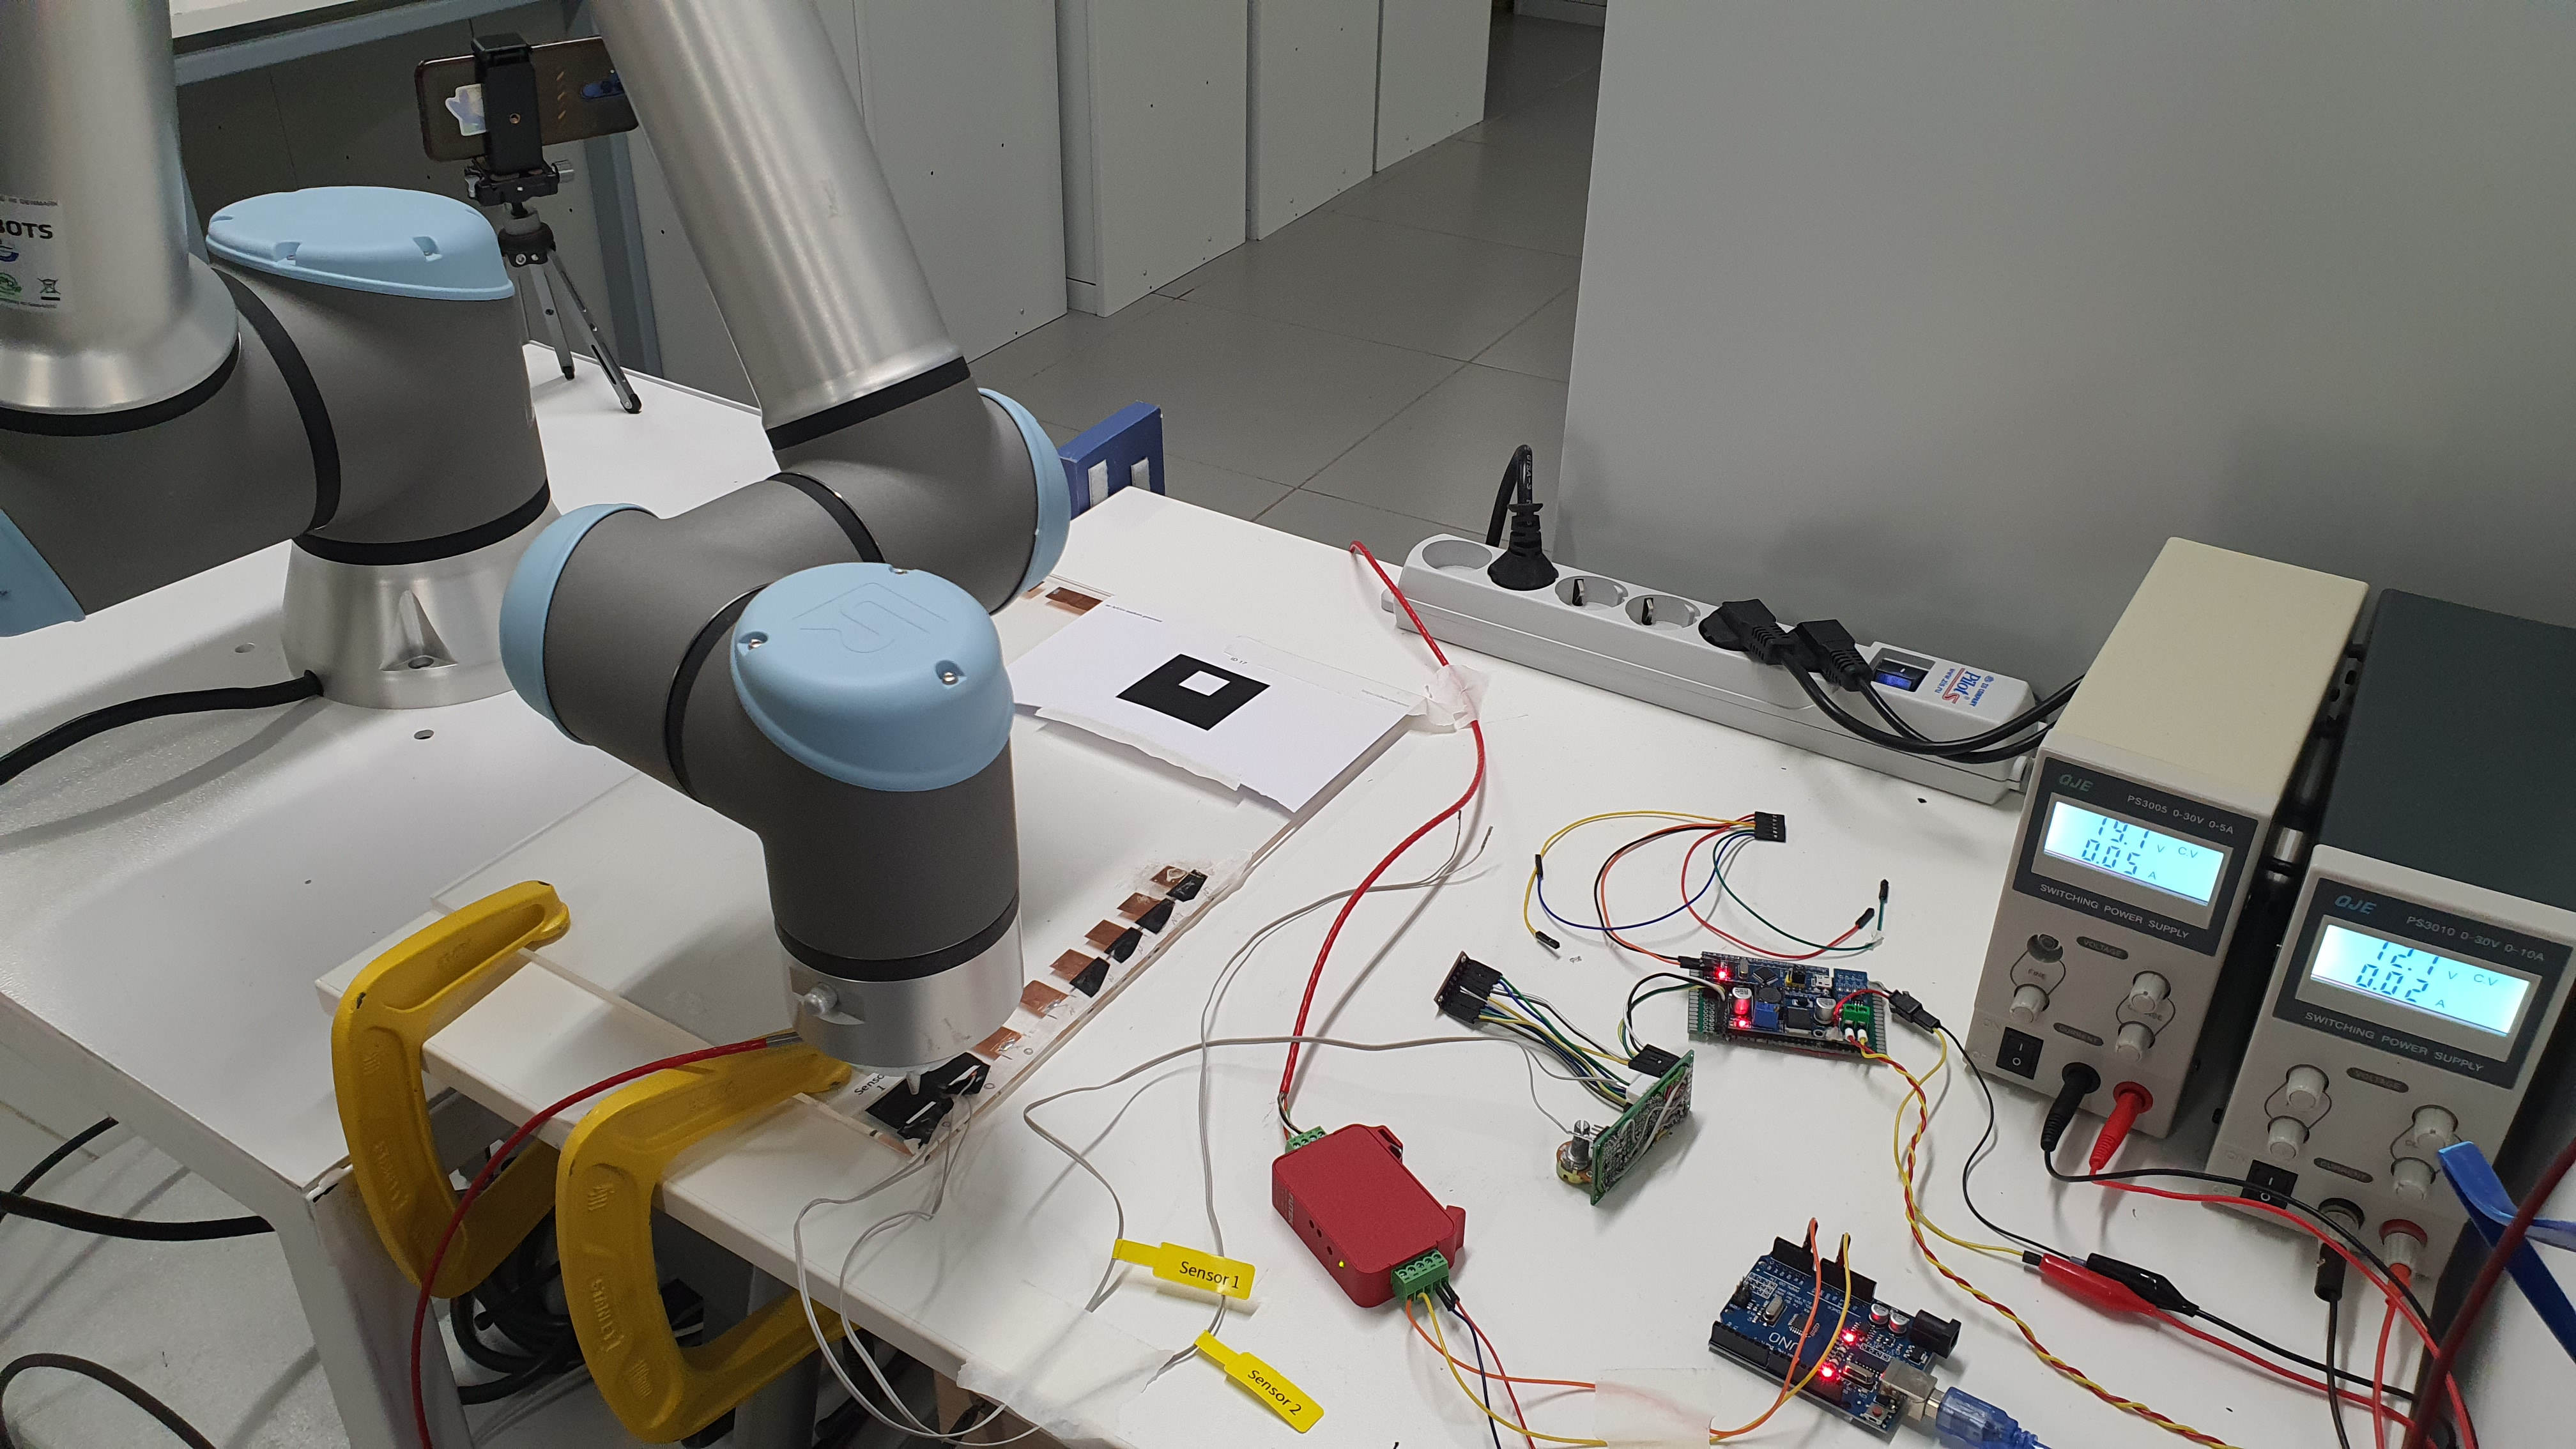
\includegraphics[height=5cm,width=1\textwidth,keepaspectratio]{exp_stand1}};

                % Create scope with normalized axes
                \begin{scope}[
                        x={($0.1*(image.south east)$)},
                        y={($0.1*(image.north west)$)}]
                    \draw[latex-, very thick,green] (3.5,2.2) -- (2.5,1)
                    node[rounded corners=3pt,below left,black,fill=white]{\small Velostat сенсор};

                    \draw[stealth-, very thick,green] (3.5,2.6) -- ++(-0.7,+0.5)
                    node[rounded corners=3pt,left,black,fill=white]{\small Датчик силы};

                    \draw[stealth-, very thick,green] (6.5,3) -- (7,6)
                    node[rounded corners=3pt,above right,black,fill=white]{\small Self-made PCB};

                    \draw[stealth-, very thick,green] (7.2,1.5) -- (8,5)
                    node[rounded corners=3pt,above right,black,fill=white]{\small Ардуино};

                    \draw[stealth-, very thick,green] (2.5,9.5) -- (4,9.5)
                    node[rounded corners=3pt,right,black,fill=white]{\small Камера};

                    \draw[very thick,green] (0.5,2.5) rectangle (4.2,9)
                    node[below left,black,fill=green]{\small UR10e};

                    \draw[latex-, very thick,green] (4.5,7.2) edge (5.5,7.5)
                    (4.8,5.3) -- (5.5,7.5)
                    node[rounded corners=3pt,above,black,fill=white]{\small Aruco маркеры};
                \end{scope}
            \end{tikzpicture}
            \caption{Общий вид экспериментального стенда}
            \label{fig:exp_standd}
        \end{subfigure}

        \begin{subfigure}{0.5\textwidth}
            \centering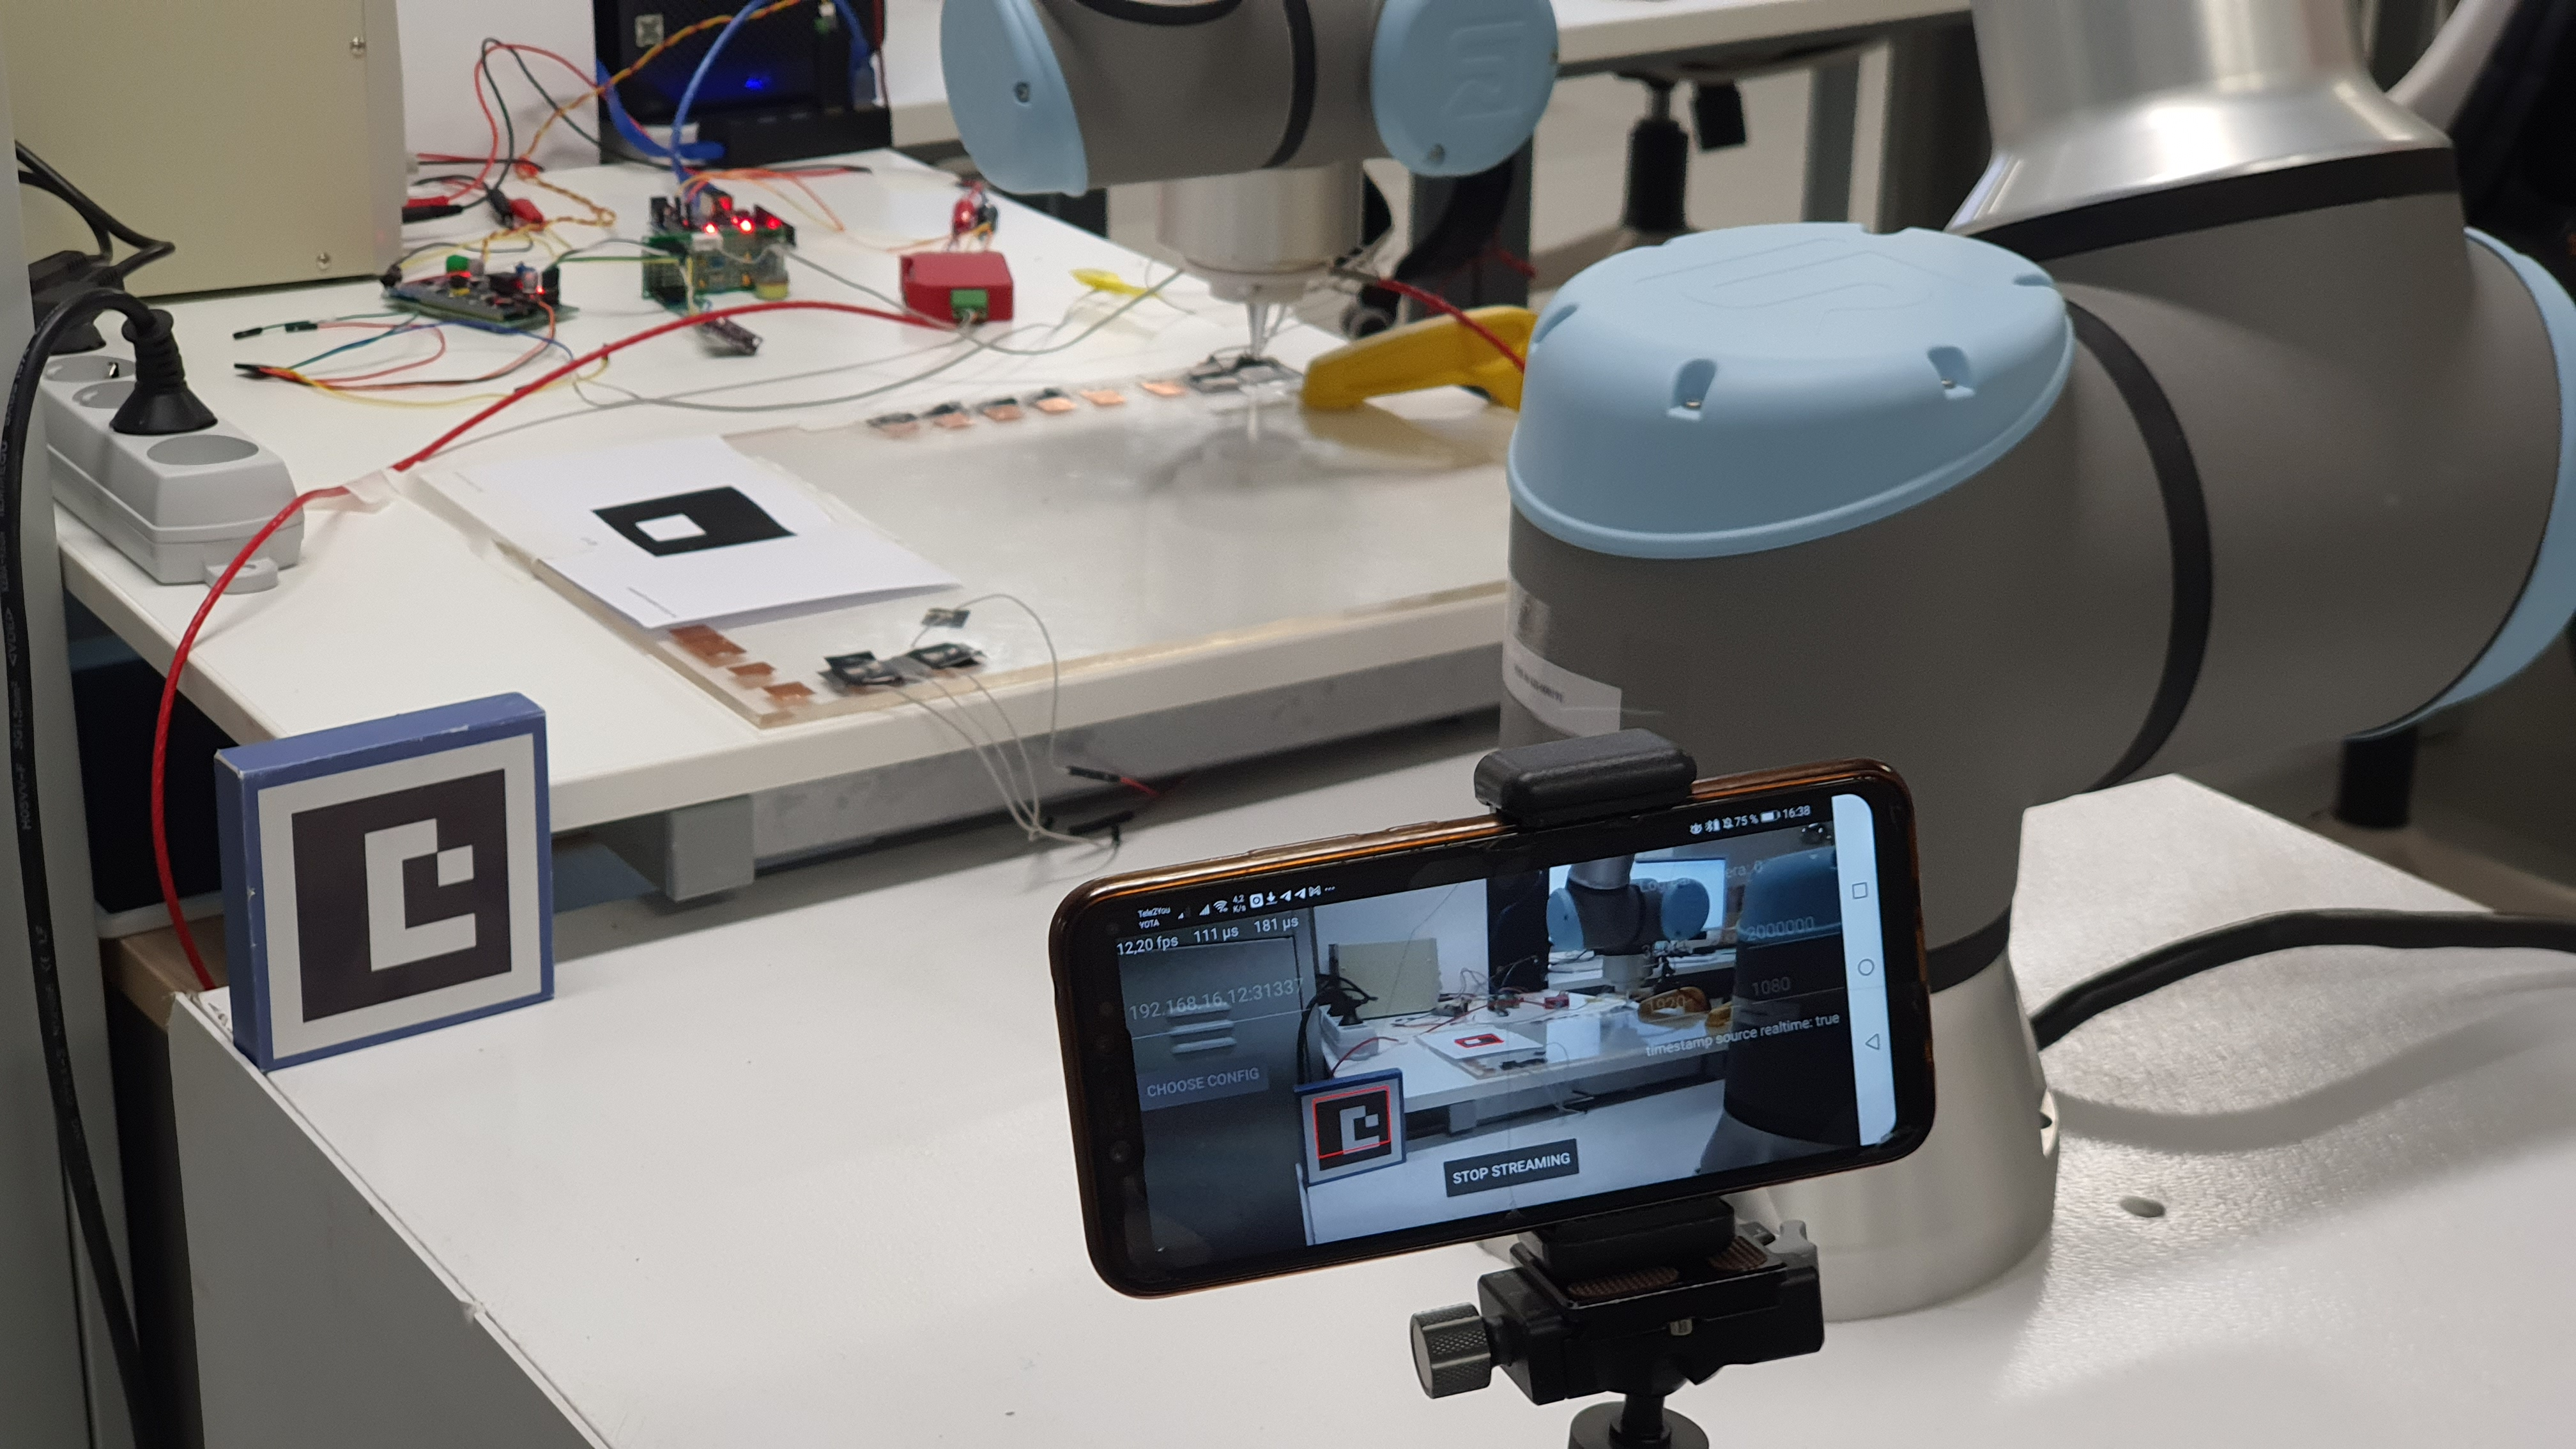
\includegraphics[height=6cm,width=1\textwidth,keepaspectratio]{exp_stand2}
            \caption{Способ нивелировать ошибку по углу с помощью Aruco маркеров}
            \label{fig:exp_stand2}
        \end{subfigure}
        \caption{Разработанный экспериментальный стенд}
    \end{center}
\end{figure}

Для касания только части объекта исследования были разработаны различные концевые инструменты. К примеру, \pic{fig:all_end_effectors.png}

\begin{figure}[h]
    \begin{subfigure}{0.6\textwidth}
        \centering
        \begin{tikzpicture}
            % Include the image in a node
            \node [above right, inner sep=0] (image) at (0,0)
            {\centering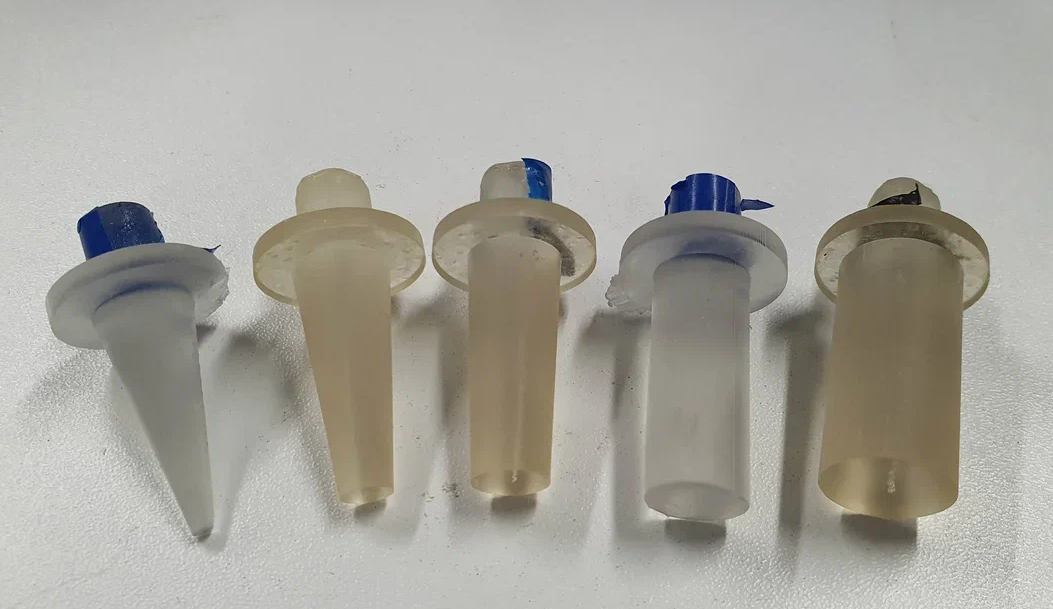
\includegraphics[height=5cm,width=1\textwidth,keepaspectratio]{all_end_effectors.png}};
            % Create scope with normalized axes
            \begin{scope}[
                    x={($ 0.1*(image.south east)$)},
                    y={($ 0.1*(image.north west)$)}]
                \node[rounded corners=3pt,black,fill=white] at (1.1,7.4){\tiny 2 mm };
                \node[rounded corners=3pt,black,fill=white] at (3.1,7.9){\tiny 6 mm };
                \node[rounded corners=3pt,black,fill=white] at (4.9,8.1){\tiny 8 mm };
                \node[rounded corners=3pt,black,fill=white] at (6.7,7.9){\tiny 12 mm };
                \node[rounded corners=3pt,black,fill=white] at (8.6,7.9){\tiny 15 mm };
            \end{scope}
        \end{tikzpicture}
        \caption{Инструмент (концевой эффектор) для нажатия объект
            исследования с диаметром нажатия меньше, чем сам объект}
        \label{fig:all_end_effectors.png}
    \end{subfigure}
    \begin{subfigure}{0.38\textwidth}
        \centering
        \begin{tikzpicture}

            % Include the image in a node
            \node [
                above right,
                inner sep=0] (image) at (0,0) {\centering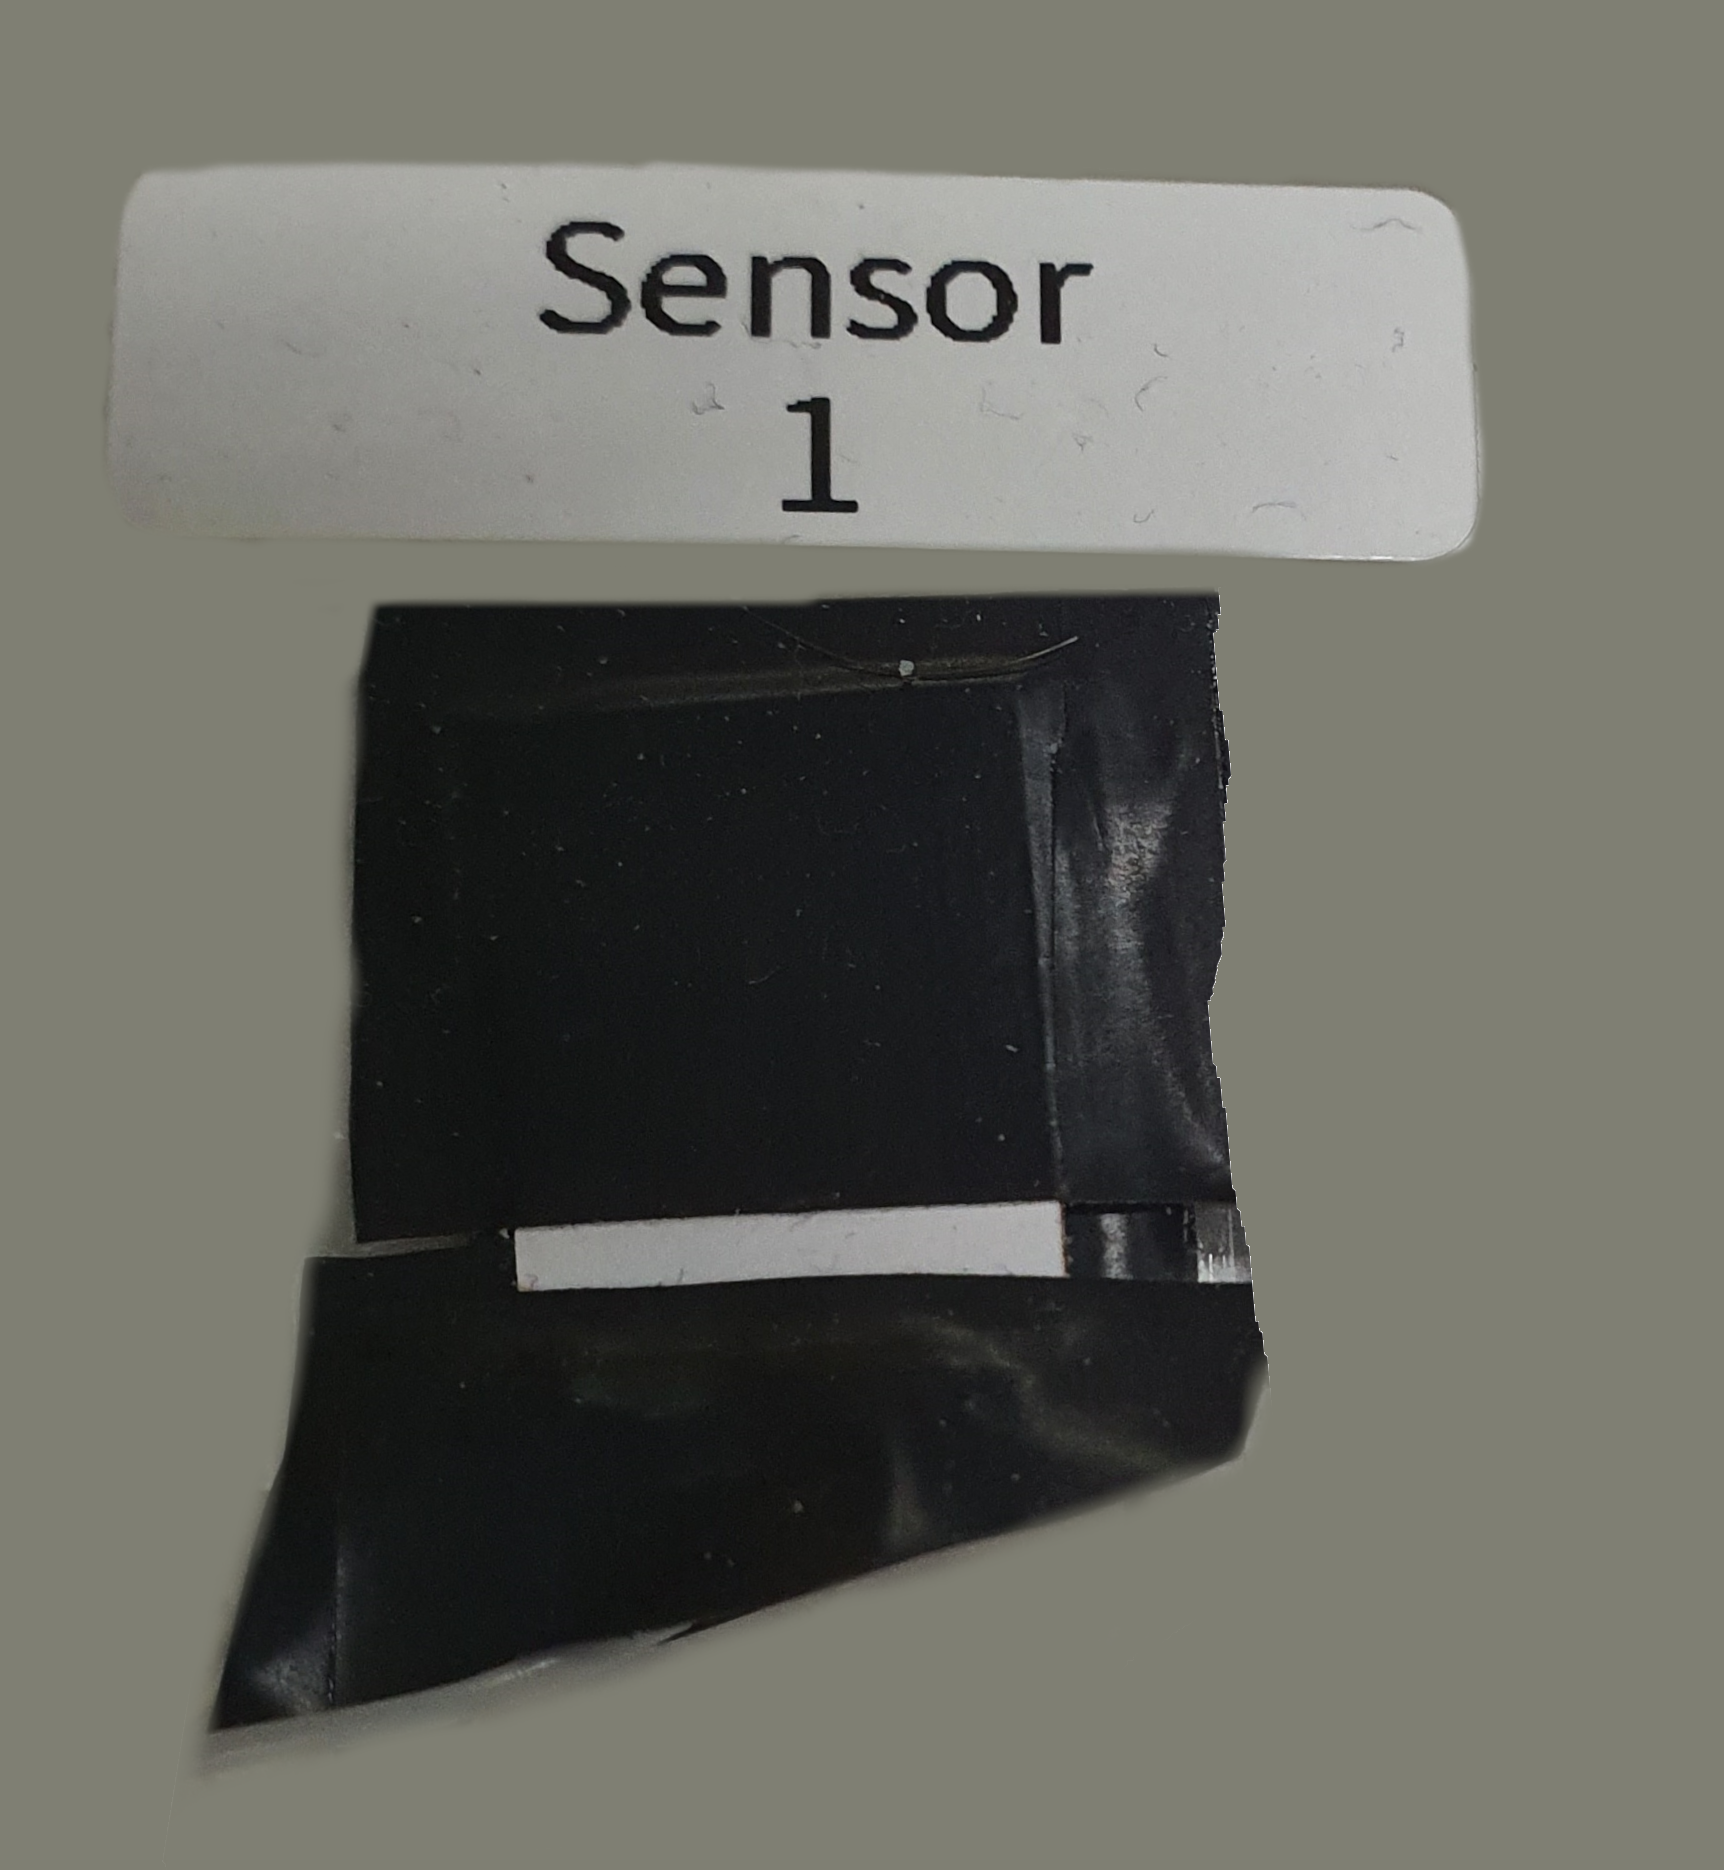
\includegraphics[height=5cm,width=1\textwidth,keepaspectratio]{sensors_grid.png}};

            % Create scope with normalized axes
            \begin{scope}[
                    x={($0.1*(image.south east)$)},
                    y={($0.1*(image.north west)$)}]
                \draw [green, very thick,
                    decorate,
                    decoration = {brace,
                            raise=5pt,
                            amplitude=5pt,
                            aspect=0.5}] (6,3.7) --  (3,3.7)
                node[pos=0.5,below=10pt,green]{$15\ mm$};

                \draw [green, very thick,
                    decorate,
                    decoration = {brace, mirror,
                            raise=5pt,
                            amplitude=5pt,
                            aspect=0.5}] (6,3.6) --  (6,6.4)
                node[pos=0.5,right=10pt,green]{$15\ mm$};

                \draw[green,step=1,xshift=34, yshift=43]  (0.5,0.5) grid +(3,3);

                \node[circle,fill=green,scale=0.4] at (3.3,6.27){\small 1};
                \node[circle,fill=green,scale=0.4] at (5.92,3.7){\small 16};
            \end{scope}

        \end{tikzpicture}
        \caption{Представление сенсора \\ как $4\times4$ сетка}
        \label{fig:sensor_grid}
    \end{subfigure}
    \caption{Представление места нажатия инструментом сенсора и сам инструмент}
\end{figure}

Impedance управление состоит из двух блоков -- модификация траектории для оси $z$, начиная с\eqref{eq:traj_mod}, и управление по скорости -- с \eqref{eq:vel_control}.

\begin{eqnarray}
    \label{eq:traj_mod}
    X_s^0 = 0, \dot{X}_s^0 =0,  X_g^k, \dot{X}_g^k \text{ -- goal state}, X_s = X_g - X_d \\
    X_g = X_g^0 + \frac{F_d}{\eta } \\
    \dot{X}_s + \eta  X_s = F^k \\
    X_s^k = odeint(X_s^{k-1},t,F^k), t = [0,dT] \\
    X_s^{k-1} = X_s^k;  \dot{X}_s = f(X_s,t,F^k) \\
    X_d = X_g - X_s; \dot{X}_d = \dot{X}_g - \dot{X}_s
\end{eqnarray}

\begin{eqnarray}
    \label{eq:vel_control}
    X_d = \begin{bmatrix}
        x_g \\ y_g \\ z_d
    \end{bmatrix} \\
    U = \dot{X}_d + K(X_d - X), \\ \text{ where } X=get\_state(); \\ 
    set\_speed(U)
\end{eqnarray}

На рисунке ниже \pic{fig:force_data_pos.png} представлен результат работы алгоритма на частоте 450 $Hz$. Необходимая сила нажатия --- $17\ H$.
\begin{figure}[h]
        \centering
         \begin{tikzpicture}
            % Include the image in a node
            \node [above right, inner sep=0] (image) at (0,0) 
            {\centering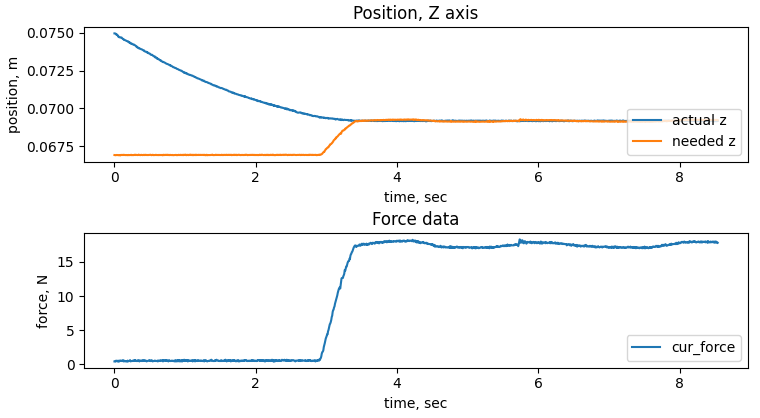
\includegraphics[height=5cm,width=1\textwidth,keepaspectratio]{force_data_pos.png}};          
            % Create scope with normalized axes
            \begin{scope}[
                x={($ 0.1*(image.south east)$)},
                y={($ 0.1*(image.north west)$)}]
                \draw[thick,green, dashed] (4.2,1) -- (4.2,8)
                node[above right,black,fill=white]{\tiny Касание с поверхностью};
            \end{scope}
        \end{tikzpicture}
        \caption{Графики зависимости силы и позиции по $z$ от времени во время эксперимента по исследованию Velostat}
        \label{fig:force_data_pos.png}
    \end{figure}


\subsection{Экспериментальная часть}
Было решено провести следующие эксперименты.
\begin{enumerate}
    \item \textbf{Статический эксперимент}. Цель — определить коэффициенты для мат. модели. Для этого на сенсор кладется известная нагрузка на 60 секунд и собираются данные с преобразователя.
          \item\textbf{Динамический эксперимент}. Цель — определить влияние показаний сенсора в зависимости от положения площадки контакта. Для этого преобразователь представляется в виде матрицы $4 \times 4$. Размер преобразователя в эксперименте 15 на 15 мм. Манипулятор нажимает на преобразователь с одинаковым давлением на протяжении всех экспериментов в различные позиции на преобразователе, используя пять различных концевых эффекторов (диаметр окружности от 2 мм до 15 мм) \pic{fig:sensor_grid}.
\end{enumerate}

Статическим экспериментом проверялась формула \eqref{eq:velostat_eqn}. Из-за гистерезиса необходимо учитывать время нажатия на объект.
\begin{eqnarray}
    \label{eq:velostat_eqn}
    V_{out} = V_0 + p[k_p + k_e(1-e^\frac{-(t-t_0)}{\tau_{res}})](1-e^{-\frac{A}{p}}) \\
    k_p = A_1e^{-A_2p}; \tau_{res} = B_0 + B_1e^{-\frac{p}{B_2}}
\end{eqnarray}
где,  $V_0$- начальное напряжение,$p,\ A_i,\ B_i,\ \tau_{res},\ k_i$  - настраиваемые константы, $t$ - текущее время, $t_0$ - время начала нажатия.
Для решения задачи регрессии использовался робастный нелинейный алгоритм наименьших квадратов. Результат представлен ниже \pic{fig:least_square_model.png}.

\begin{figure}[H]
    \centering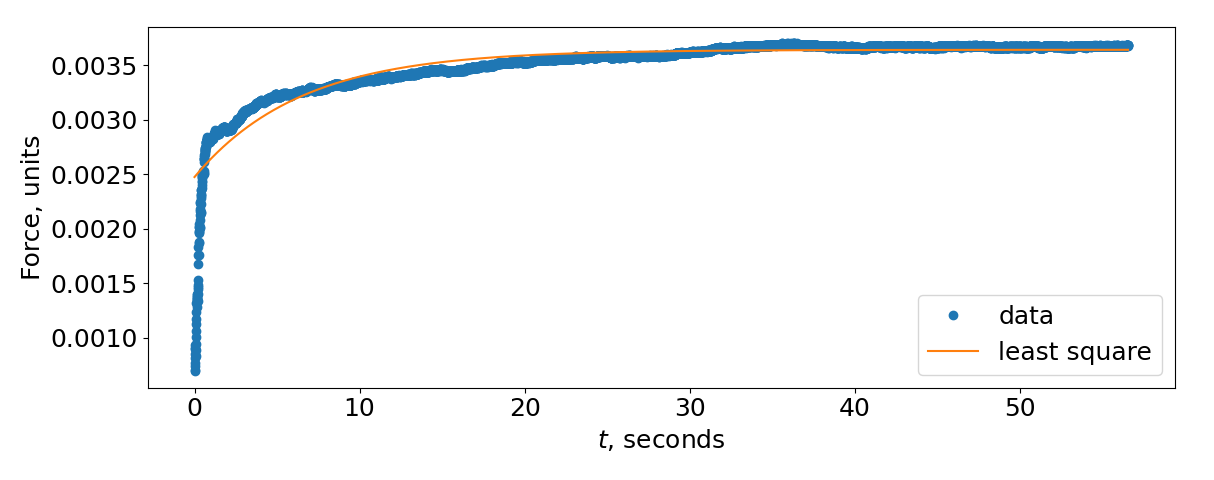
\includegraphics[height=2.8cm,width=1\textwidth,keepaspectratio]{least_square_model.png}
    \caption{Результаты статического эксперимента}
    \label{fig:least_square_model.png}
\end{figure}

Ниже \pic{fig:dynamics_exp} представлены некоторые результаты распределения ошибок по площади сенсора при взаимодействии с концевыми эффекторами разных размеров. Ошибки определялись как разница между показаниями калиброванного сенсора силы Futek и исследуемого преобразователя на базе Velostat. На рисунке \ref{fig:sens1_pike1} показаны ошибки для концевого эффектора диаметром 2 мм, а на рисунке \ref{fig:sens1_pike3} — для концевого эффектора диаметром 8 мм.

Можно заметить, что в \ref{fig:sens1_pike3} максимальная разница между Futek и Velostat не более 0.2 в одном месте. Остальные элементы сетки не превышают 10\%. Такая же тенденция продолжается как и при увеличении размера концевого эффектора, так и на других сенсорах.

\begin{figure}[H]
    \begin{subfigure}{0.49\textwidth}
        \centering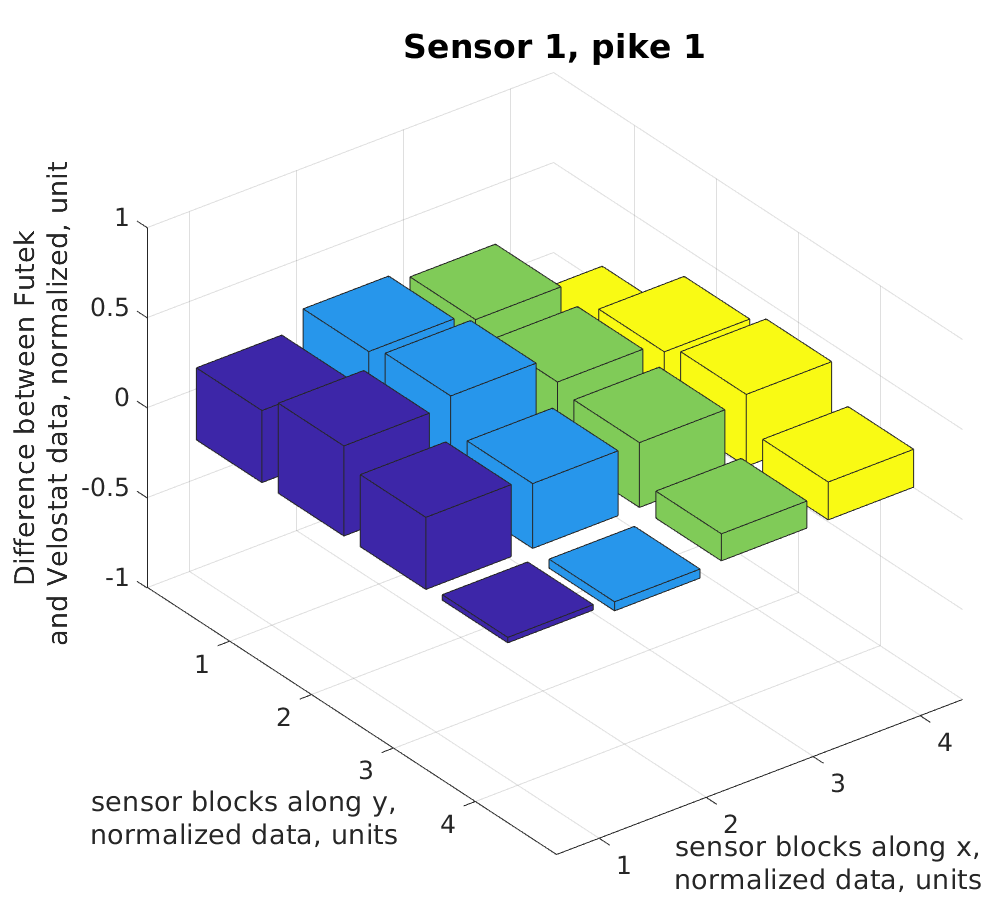
\includegraphics[height=4cm,width=1\textwidth,keepaspectratio]{sens1_pike1.png}
        \caption{диаметр концевого эффектора равный 2 мм }
        \label{fig:sens1_pike1}
    \end{subfigure}
    \begin{subfigure}{0.49\textwidth}
        \centering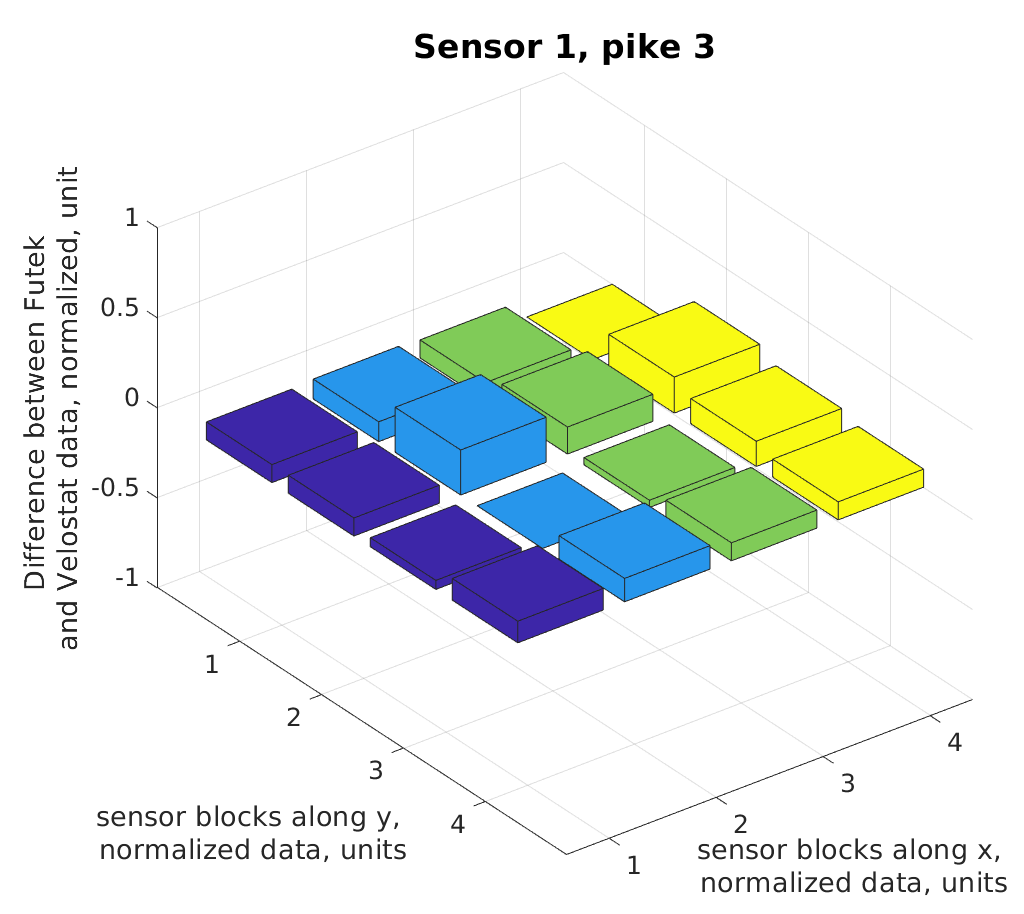
\includegraphics[height=4cm,width=1\textwidth,keepaspectratio]{sens1_pike3.png}
        \caption{Диаметр концевого эффектора равный 8 мм }
        \label{fig:sens1_pike3}
    \end{subfigure}
    \caption{Динамический эксперимент}
    \label{fig:dynamics_exp}
\end{figure}

\subsection{Вывод}
По результатам исследований показано, что характеристики преобразователя удовлетворяют требованиям к системе тактильного восприятия шагающего робота, когда ожидаемый размер площади контакта превышает половину размера преобразователя.

\textbf{\underline{Четвертая глава}} раскрывает детали определения профиля опорной поверхности, на основе информации о точках её касания ногами робота и внутренних датчиков, характеризующих механическое состояние аппарата. Вторая часть главы показывает определение с помощью робота физико-механических свойств опорной поверхности:
жесткости, упругости и пластичности.

\textbf{Первая задача:} имеется поверхность. Каждому набору координат $x,\ y$ соответствует одно и только одно значение координаты $z$. Необходимо с помощью ощупывания роботом поверхности получить плотное облако точек и полигональную сетку. 

Сделано предположение, что расстояние между ногами робота мало относительно размеров поверхности, следовательно, поверхность между ногами считается плоскостью.

Для получения облака точек касаний опорных поверхностей, относительно глобальной системы координат, необходима трансформация систем координат от глобальной, до конкретного сенсора на ноге. Этому соответствует прямая задача кинематики \pic{fig:StriRus_10_legs_15_angle_v4.png}, \eqref{eq:forw_kin} и задачи локализации.

\begin{figure}[H]
    \centering
     \begin{tikzpicture}
        % Include the image in a node
        \node [above right, inner sep=0] (image) at (0,0) 
        {\centering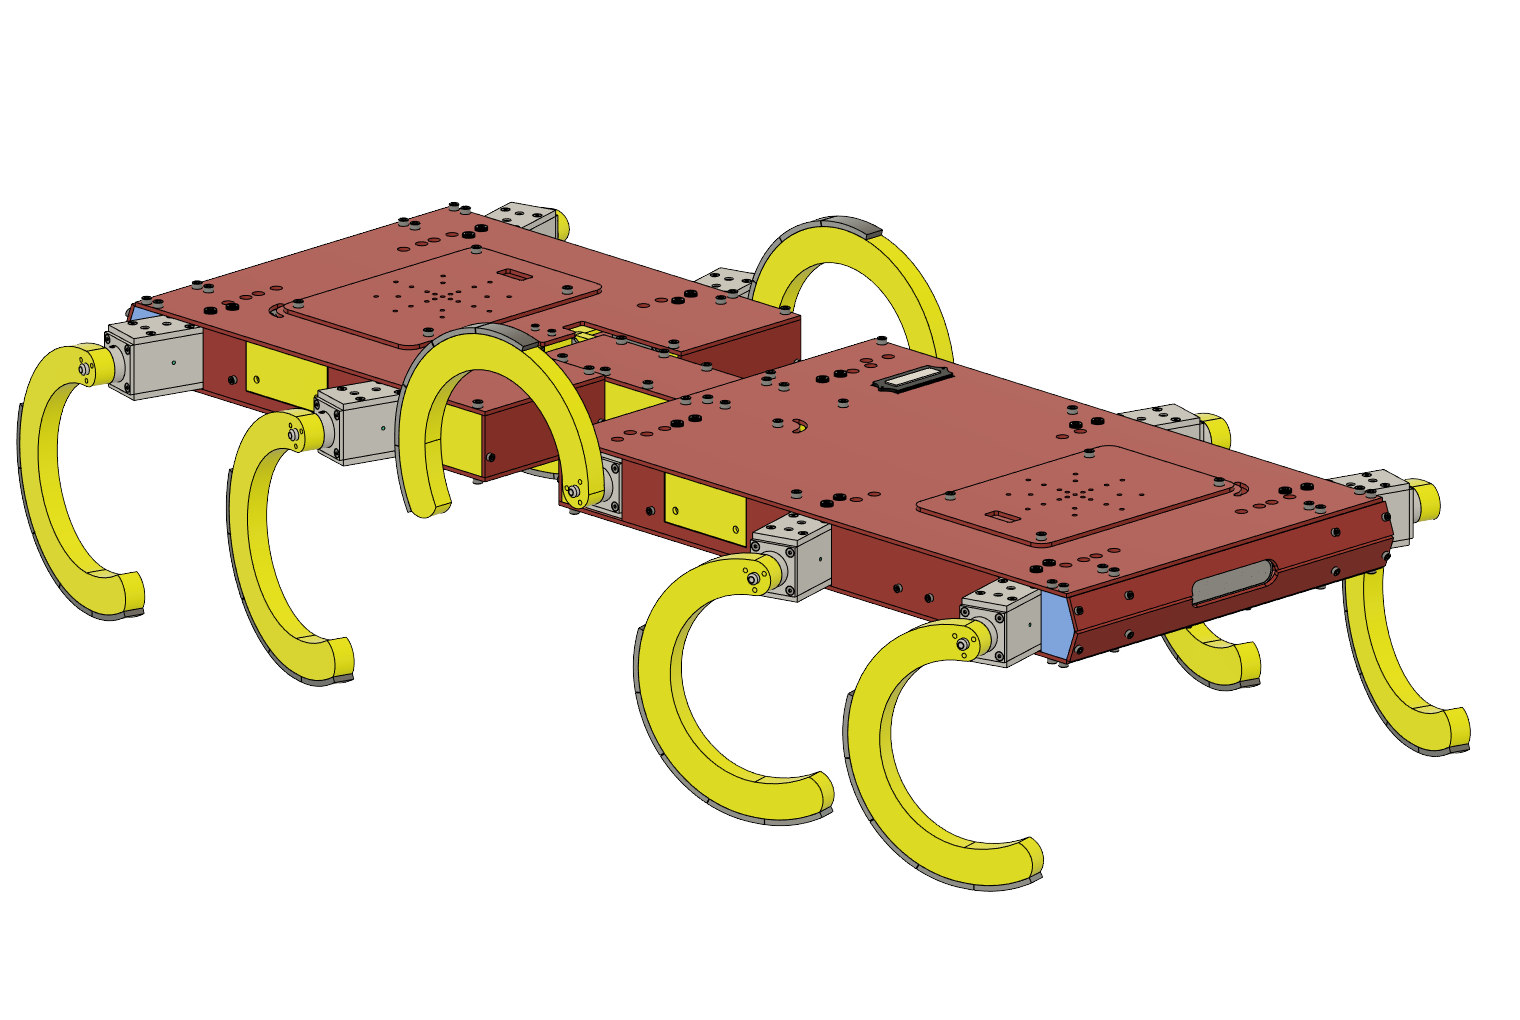
\includegraphics[height=5.5cm,width=1\textwidth,keepaspectratio]{StriRus_10_legs_15_angle_v4.png}};          
        % Create scope with normalized axes
        \begin{scope}[
            x={($ 0.1*(image.south east)$)},
            y={($ 0.1*(image.north west)$)}]
            % Grid and axes' labels
            % \draw[lightgray,step=1] (image.south west) grid (image.north east);
            % \foreach \x in {0,1,...,10} { \node [below] at (\x,0) {\x}; }
            % \foreach \y in {0,1,...,10} { \node [left] at (0,\y) {\y};}
 
            % Labels

            \coordinate (Xc) at (0.4415/2,-0.2347/2);
            \coordinate (Yc) at (-0.4512/2,-0.2156/2);
            \coordinate (Zc) at (0,0.5/2);
            % Labels
            \tikzstyle{origin} = [rounded corners=2pt, black, fill=gray!40, fill opacity=0.75, text opacity=1, scale=0.8,inner sep=1pt]
            \tikzstyle{transform_text} = [rounded corners=2pt, black, fill=white!85!gray, fill opacity=0.75, text opacity=1, scale=0.8,inner sep=1pt]
            \tikzstyle{transform_arrow} = [thick, green]
    
            % \coordinate (o_g) at (1,9);
            \node[circle,fill=green,scale=0.25] (o_g) at (1,9){};
            \draw[-stealth, very thick,blue] (o_g) -- ++(Xc);
            \draw[-stealth, very thick,green!70!black] (o_g) -- ++(Yc);
            \draw[-stealth, very thick,red] (o_g) -- ++(Zc);
            \node[origin,above right=3pt] at (o_g){\tiny $\mathbf{O_{glob}}$};
    
            % \coordinate (o_b) at (2.9,7.05);
            \node[circle,fill=green,scale=0.25] (o_b) at (2.9,7.05){};
            \draw[-stealth, very thick,blue] (o_b) -- ++(Xc);
            \draw[-stealth, very thick,green!70!black] (o_b) -- ++(Yc);
            \draw[-stealth, very thick,red] (o_b) -- ++(Zc);
            \node[origin,above right=2pt] at (o_b){\tiny $\mathbf{O_{base}}$};
    
            % \coordinate (o_1) at (2.9,6.6);
            \node[circle,fill=green,scale=0.25] (o_1) at (2.9,6.6){};
            \draw[-stealth, very thick,blue] (o_1) -- ++(Xc);
            \draw[-stealth, very thick,green!70!black] (o_1) -- ++(Yc);
            \draw[-stealth, very thick,red] (o_1) -- ++(Zc);
            \node[origin,above right=2pt] at (o_1){\tiny $\mathbf{O_{1}}$};
    
            % \coordinate (o_2) at (4,6);
            \node[circle,fill=green,scale=0.25] (o_2) at (4,6){};
            \draw[-stealth, very thick,blue] (o_2) -- ++(Xc);
            \draw[-stealth, very thick,green!70!black] (o_2) -- ++(Yc)
            node[origin,below=2pt]{\tiny $\mathbf{\alpha_3}$};
            \draw[-stealth, very thick,red] (o_2) -- ++(Zc);
            \node[origin,above right=2pt] at (o_2){\tiny $\mathbf{O_{2}=O_{3}}$};
    
            % \coordinate (o_4) at (7.0,4.55);
            \node[circle,fill=green,scale=0.25] (o_4) at (7.0,4.55){};
            \draw[-stealth, very thick,blue] (o_4) -- ++(Xc);
            \draw[-stealth, very thick,green!70!black] (o_4) -- ++(Yc);
            \draw[-stealth, very thick,red] (o_4) -- ++(Zc);
            \node[origin,above right=2pt] at (o_4){\tiny $\mathbf{O_{4}}$};
    
            % \coordinate (o_5) at (6.7,4.45);
            \node[circle,fill=green,scale=0.25] (o_5) at (6.7,4.45){};
            \draw[-stealth, very thick,blue] (o_5) -- ++(Xc);
            \draw[-stealth, very thick,green!70!black] (o_5) -- ++(Yc);
            \draw[-stealth, very thick,red] (o_5) -- ++(Zc);
            \node[origin,above left=3pt] at (o_5){\tiny $\mathbf{O_{5}=O_{6}}$};
    
            \coordinate (Xcr) at (0.49/2,0.07/2);
            % \coordinate (Ycr) at (-0.38/2,-0.32/2);
            \coordinate (Ycr) at (-0.24/2,-0.43/2);
    
            \draw[-stealth, very thick,blue] (o_5) -- ++(Xcr);
            \draw[-stealth, very thick,green!70!black] (o_5) -- ++(Ycr);
    
    
            % \coordinate (o_7) at (6.36,3.68);
            \node[circle,fill=green,scale=0.25] (o_7) at (6.36,3.68){};
            \draw[-stealth, very thick, blue] (o_7) -- ++(Xcr);
            \draw[-stealth, very thick, green!70!black] (o_7) -- ++(Ycr)
            node[origin,above left=2pt]{\tiny $\mathbf{\alpha_8}$};
            \draw[-stealth, very thick, red] (o_7) -- ++(Zc);
            \node[origin,below right=3pt] at (o_7){\tiny $\mathbf{O_{7}=O_{8}}$};
    
            \node[circle, draw ,fill=green,scale=0.4] (s_1) at (6.6,1.3){1};
            \node[circle,draw, fill=green,scale=0.4] (s_3) at (5.85,1.7){3};
            \node[circle,draw, fill=green,scale=0.4] (s_5) at (5.55,2.9){5};
    
            \draw[-stealth, transform_arrow] (o_g) -- (o_b)
            node[midway,below left=2pt, transform_text]{\tiny $\mathbf{H_{base}^{glob}}$};
    
            \draw[-stealth, transform_arrow] (o_b) -- (o_1)
            node[midway,left=3pt, transform_text]{\tiny $\mathbf{H_{1}^{base}}$};
    
            \draw[-stealth, transform_arrow] (o_1) -- (o_2)
            node[midway,below=2pt, transform_text]{\tiny $\mathbf{H_{2}^{1}}$};
    
            \draw[-stealth, transform_arrow] (o_2) -- (o_4)
            node[midway,below=2pt, transform_text]{\tiny $\mathbf{H_{4}^{3}}$};
    
            \draw[-stealth, transform_arrow] (o_4) -- (o_5)
            node[midway,below right=2pt, transform_text]{\tiny $\mathbf{H_{5}^{4}}$};
    
            \draw[-stealth, transform_arrow] (o_5) -- (o_7)
            node[midway,left=3pt, transform_text]{\tiny $\mathbf{H_{7}^{6}}$};
    
            \draw[-stealth, transform_arrow] (o_7) -- (s_1);
            \draw[-stealth, transform_arrow] (o_7) -- (s_3);
            \draw[-stealth, transform_arrow] (o_7) -- (s_5);
        \end{scope}
    \end{tikzpicture}
    \caption{Кинематическая схема для определения точки касания опорной поверхности роботом}
    \label{fig:StriRus_10_legs_15_angle_v4.png}
\end{figure}

\begin{multline}
    \label{eq:forw_kin}
        H_{leg}^{glob} = H(x_{glob},y_{glob},z_{glob},\alpha_{glob},\beta_{glob},\gamma_{glob})T_z(l_1)\\ T_x(l_2)R_y(\alpha_3)T_x(l_4)T_y(l_5)R_z(-15^{\circ})T_y(l_7)R_y(\alpha_8)
\end{multline}
Где каждая матрица представляет собой матрицу однородного преобразования, через $R_i$ обозначены однородные матрицы поворота, относительно соответствующей осеи, $T_i$ --- однородную матрицу перемещения.

Для получения плотного облака точек необходимо очистить оригинальное облако точек от шумов и усреднить близлежащие точки с помощью Voxel grid. Потом из него генерируется полигональная сетка с помощью 2D Триангуляции Делоне \pic{fig:delone_idea.png} (вогнутая оболочка \pic{fig:exp_concave_hull}). На ее основе получается необходимое плотное облако точек. 

\begin{figure}[ht!]
    \centering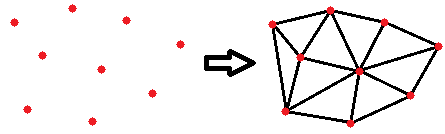
\includegraphics[height=2.5cm,width=1\textwidth,keepaspectratio]{delone_idea.png}
    \caption{2D Триангуляция Делоне (выпуклая оболочка)}
    \label{fig:delone_idea.png}
\end{figure}

Модификация триангуляции Делоне нужна, так как выпуклой оболочке \pic{fig:conv_convex.png} алгоритм построил карту местности там, где робот не ходил. При использовании вогнутой оболочки \pic{fig:conv_concave.png} данная проблема не наблюдается.

\begin{figure}[H]
    \begin{subfigure}[t]{0.32\textwidth}
        \centering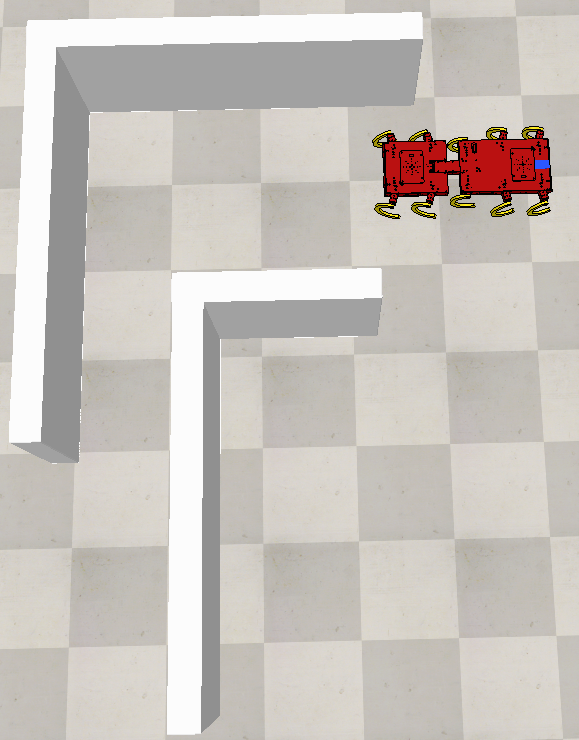
\includegraphics[height=3cm,width=1\textwidth,keepaspectratio]{convex_terr.png}
        \caption{Пример поля}
        \label{fig:convex_terr.png}
    \end{subfigure}
    \begin{subfigure}[t]{0.32\textwidth}
        \centering
        \begin{tikzpicture}
            % Include the image in a node
            \node [above right, inner sep=0] (image) at (0,0)
            {\centering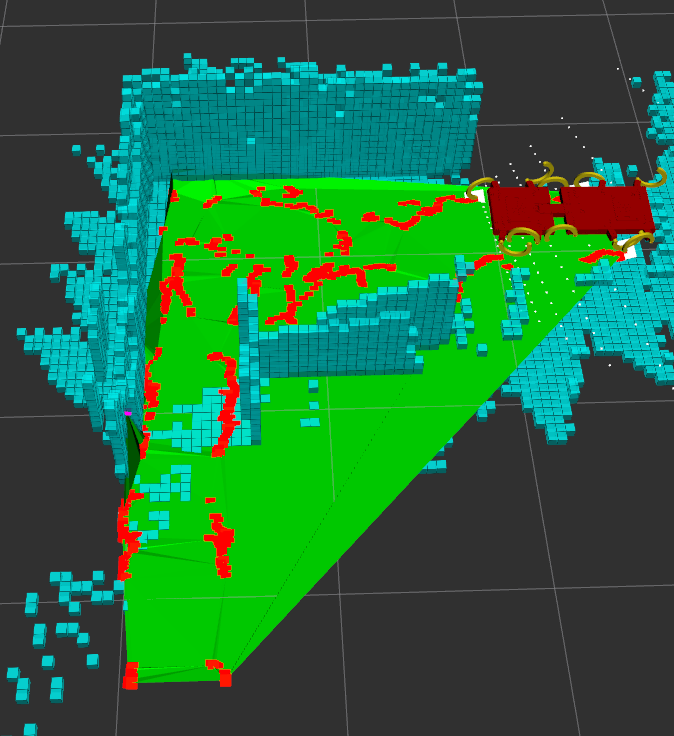
\includegraphics[height=4cm,width=1\textwidth,keepaspectratio]{conv_convex.png}};
            % Create scope with normalized axes
            \begin{scope}[
                x={($ 0.1*(image.south east)$)},
                y={($ 0.1*(image.north west)$)}]
            % Labels
            \draw[stealth-, very thick,green] (5.2,3.5) -- ++(0,-1)
            node[rounded corners=3pt,right,black,fill=white]{\tiny Полученная сетка};

            \draw[stealth-, very thick,green] (5.5,5.5) -- (6.4,4)
            node[rounded corners=3pt,right,black,fill=white]{\tiny Данные лидара};


            \draw[stealth-, very thick,green] (3.4,0.8) -- (5,1);
            \draw[stealth-, very thick,green] (3.4,2.6) -- (5,1)
            node[rounded corners=3pt,right,black,fill=white]{\tiny Следовая дорожка};
        \end{scope}
        \end{tikzpicture}
        \caption{Выпуклая оболочка}
        \label{fig:conv_convex.png}
    \end{subfigure}
    \begin{subfigure}[t]{0.32\textwidth}
        \centering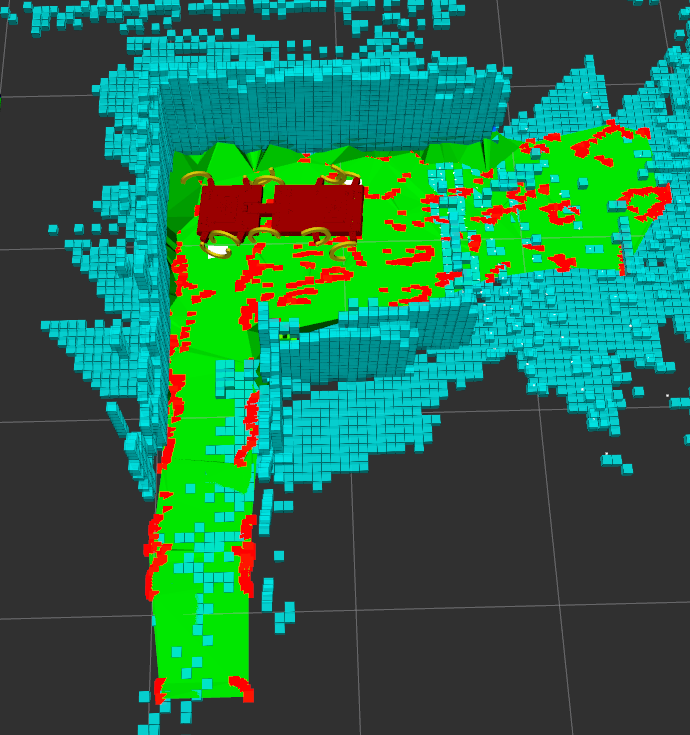
\includegraphics[height=4cm,width=1\textwidth,keepaspectratio]{conv_concave.png}
        \caption{Вогнутая оболочка}
        \label{fig:conv_concave.png}
    \end{subfigure}
    \caption{Объяснение необходимости модификации алгоритма Делоне}
    \label{fig:exp_concave_hull}
\end{figure}

Проверка алгоритма в симуляции (Рис. \ref{fig:unsolvable_case}), натурно \pic{fig:real_exp_map_creation}.

\begin{figure}[H]
    \begin{subfigure}[t]{0.49\textwidth}
            \centering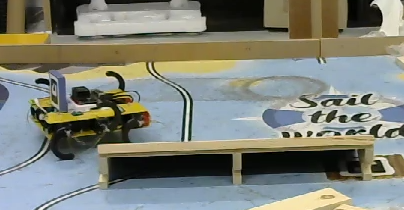
\includegraphics[height=6cm,width=1\textwidth,keepaspectratio]{real_robot_mesh_video_preview.png}
        \caption{Робот проходит препятствие}
        \label{fig:real_robot_mesh_video_preview.png}
    \end{subfigure}
    \begin{subfigure}[t]{0.49\textwidth}
        \centering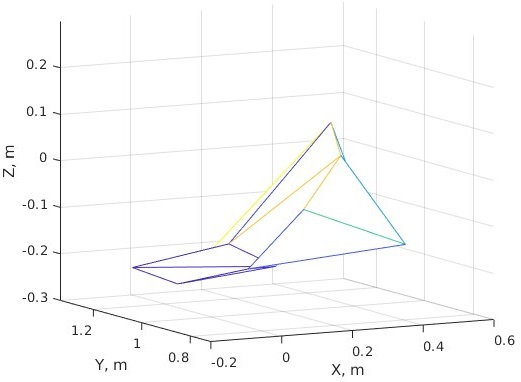
\includegraphics[height=3cm,width=1\textwidth,keepaspectratio]{real_mesh.jpg}
        \caption{Полученная полигональная сетка}
        \label{fig:real_mesh.jpg}
    \end{subfigure}
    \caption{Пример натурного эксперимента}
    \label{fig:real_exp_map_creation}
\end{figure}

Для оценки точности полученных данных использовались метрики Cloud to Cloud (C2C) \eqref{eqn:hauff} и Cloud to Mesh (C2M) \pic{fig:metrics}.

\begin{equation}
    \label{eqn:hauff}
    d_{H}(X,\;Y)=\sup _{m\in M}\left\{\,|\mathrm {dist} _{X}(m)-\mathrm {dist} _{Y}(m)|\,\right\}    
\end{equation}
Где $X,\ Y$ непустые подмножества метрического пространства $M$; $\mathrm {dist} _{X}\colon M\to \mathbb {R}$ $\mathrm {dist} _{X}\colon M\to \mathbb {R}$ обозначает функцию расстояния до множества $X$.


\begin{figure}[ht!]
    \begin{subfigure}[t]{0.49\textwidth}
        \centering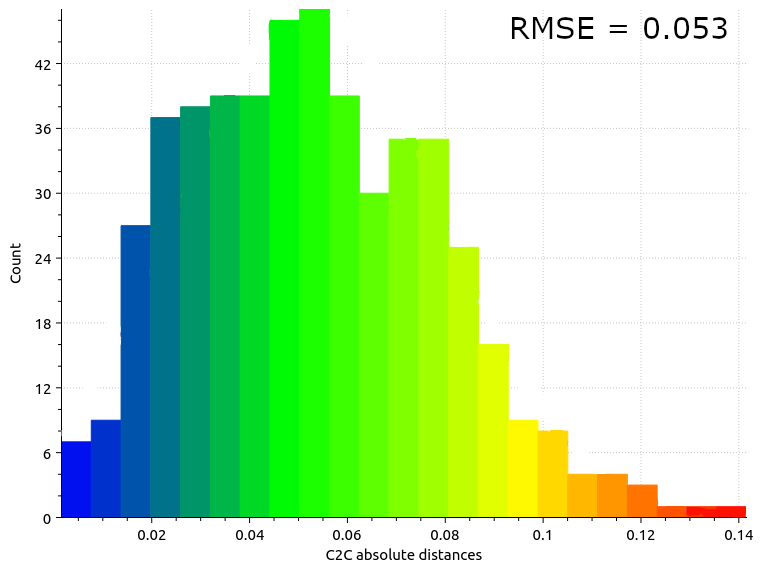
\includegraphics[height=3.5cm,width=1\textwidth,keepaspectratio]{pcd_hist.png}
        \caption{Метрика C2C: гистограмма ошибок (абсолютное расстояние от точки до ближайшей реферальной точки)}
        \label{fig:metric_c2c}
    \end{subfigure}
    \begin{subfigure}[t]{0.49\textwidth}
        \centering\includegraphics[height=3.5cm,width=1\textwidth,keepaspectratio]{mesh_hist.png}
        \caption{Метрика C2M: Гистограмма ошибок (относительное расстояние от точки до ближайшей реферальной точки)}
        \label{fig:metric_c2m}
    \end{subfigure}
    \caption{Метрики оценки точности полученной карты}
    \label{fig:metrics}
\end{figure}


Как итог, среднеквадратичная ошибка для C2C метрики была в среднем равна 5 см. А для C2M 1 см. В натурном эксперименте по метрике C2C --- 8 см.

\textbf{Вторая задача} это определение физико-механических свойств опорной поверхности. С точки зрения механики свойства поверхности с водятся к показателям упругости, вязкости и пластичности. Однако непосредственное измерение этих показателей затруднительно. В исследовании решалась задача классификации опорной поверхности с помощью искусственной нейронной сети. В качестве эталона жёсткой поверхности использовались крупные камни, эталоном упругой поверхности была принята резина, а эталоном поверхности с явно выраженными свойствами пластичности выступила песчаная почва. 

При движении робота по поверхности собираются данные с датчиков силы и с моторов. На основе предварительного обучения с помощью метода опорных векторов (SVM), данные обрабатываются и классифицируется.

Вектор с входными данными представлен следующим образом:
\begin{itemize}
    \item Элемент(1) --- Частота движения ног
    \item (2) --- Пиковая амплитуда давления с датчика силы
    \item (3) --- Ширина давления с датчика силы. Это расстояние между началом и концом акта движения. Такие отрезки складываются и получается ширина.
    \item (4) --- Площадь под кривой силы датчика
    \item (5) --- Пиковая амплитуда крутящего момента двигателя
    \item (6) --- Пиковый крутящий момент двигателя
    \item (7) --- Среднее давление на сенсорах
    \item (8) --- Средняя амплитуда крутящего момента
    \item (9) --- Средний крутящий момент двигателя
    \item (10) --- Ширина крутящего момента двигателя
    \item (11) --- Площадь под кривой крутящего момента двигателя
    \item (12-16) --- Индивидуальная пиковая амплитуда силы датчика силы 
\end{itemize}

В качестве причин выбора таких входных данных можно отметить следующие. Видно различное поведение сенсоров в зависимости от типа поверхности \pic{fig:s_shape_leg/TaxelIndForce_full.png}. Зависимость средней линейной скорости движения ноги на разных поверхностях при различных угловых скоростях \pic{fig:s_shape_leg/avg_lin_vel_rev_min.png}. 


\begin{figure}[ht!]
    \begin{subfigure}{0.99\textwidth}
        \centering\includegraphics[height=4.5cm,width=1\textwidth,keepaspectratio]{s_shape_leg/TaxelIndForce.png}
        \caption{Запись активных датчиков силы на разных поверхностях}
        \label{fig:s_shape_leg/TaxelIndForce_full.png}
    \end{subfigure}

    \begin{subfigure}{0.99\textwidth}
        \centering\includegraphics[height=3.5cm,width=1\textwidth,keepaspectratio]{s_shape_leg/avg_lin_vel_rev_min.png}
        \caption{Средняя линейная скорость робота}
        \label{fig:s_shape_leg/avg_lin_vel_rev_min.png}
    \end{subfigure}

\caption{Причины использования конкретных входных данных}
\end{figure}

В процессе обучения собранные данные были разделены на обучающее (80\% данных) и тестовое множества (20\%). Модель была обучена с использованием ядра на основе функции Пирсона VII (PUK). 

Для оценки эффективности модели использовался тестовый набор. Производительность измерялась с точки зрения точности классификации и F1-score.

Функция принятия решения для SVM-модели \eqref{eq:SVM}:

\begin{align}
    \label{eq:SVM}
    f(x) = w^T x + b
\end{align}

где $x$ --- входной вектор, $w$ является весовым вектором, и $b$ --- смещение.

Универсальное ядро на основе функции Пирсона VII \eqref{eq:PUK}:

\begin{align}
    \label{eq:PUK}
    K(x, y) = (1 + ((||x - y||^2)/\sigma^2)^\omega)^{(-1/\omega)}
\end{align}
Где $x$, $y$ --- векторы во входном пространстве, $||x - y|||$ обозначает евклидово расстояние между $x$ и $y$, $\sigma$ --- масштабный параметр, определяющий <<разброс>> ядра, $\omega$ --- это параметр формы, который влияет на форму границы принятия решения.

Данные собирались с установки, которая разрабатывалась так, чтобы было возможно быстро сменить тип поверхности, нога робота бесконечно могла совершать движения и узел с ногой был таким же как на реальном роботе \pic{fig:s_shape_leg/s_leg_setup.JPG}.

\begin{figure}[H]
    \begin{subfigure}{0.39\textwidth}
        \centering
        \begin{tikzpicture}
            % Include the image in a node
            \node [above right, inner sep=0] (image) at (0,0)
            {\centering\includegraphics[height=5cm,width=1\textwidth,keepaspectratio]{s_shape_leg/s_leg_setup.JPG}};
            % Create scope with normalized axes
            \begin{scope}[
                x={($ 0.1*(image.south east)$)},
                y={($ 0.1*(image.north west)$)}]
            \draw[stealth-, very thick,green] (3.5,2.5) -- (3,1.5)
            node[rounded corners=3pt,below,black,fill=white]{\tiny Стол для поверхностей};
    
            \draw[stealth-, very thick,green] (7.1,5.4) -- (7.4,7)
            node[rounded corners=3pt,above right,black,fill=white]{\tiny Контроллер};
    
            \draw[very thick,green] (6,6.1) rectangle (8.5,3.5)
            node[above left,black,fill=green]{\tiny S leg};
        \end{scope}
        \end{tikzpicture}
        \caption{Общий вид экспериментальной установки}
    \end{subfigure}
        \begin{subfigure}{0.20\textwidth}
            \centering\includegraphics[height=5cm,width=1\textwidth,keepaspectratio]{s_shape_leg/socks_new.jpg}
            \caption{Расположение сенсоров на ноге робота}
            \label{fig:s_shape_leg/socks.jpg}
        \end{subfigure}
        \begin{subfigure}{0.39\textwidth}
            \centering\includegraphics[height=5cm,width=1\textwidth,keepaspectratio]{s_shape_leg/leg_design.png}
            \caption{Схематическое расположение сенсоров на ноге установки}
            \label{fig:s_shape_leg/leg_design.png}
        \end{subfigure}

    \caption{Экспериментальная установка}
    \label{fig:s_shape_leg/s_leg_setup.JPG}
\end{figure}


Результат обучения представлен в виде таблицы \tab{tabular:prob_terrain_classification}.

\begin{table}[H]
    \caption{Вероятность определения типа поверхности}
    \label{tabular:prob_terrain_classification}
    \centering
\begin{tabular}{|c|c|c|c|c|} 
    \cline{3-5}
    \multicolumn{1}{l}{} & \multicolumn{1}{l|}{} & \multicolumn{3}{c|}{\textbf{Предсказанный класс}} \\ 
    \cline{3-5}
    \multicolumn{1}{l}{} &  & Камень & Резина & Земля \\ 
    \hline
    \multirow{3}{*}{{\textbf{Истинный класс}}} & Камень & {\cellcolor[rgb]{0.741,0.843,0.929}}84.0\% & 2.56\% & 13.44\% \\ 
    \hhline{|~----|}
     & Резина & 20.1\% & {\cellcolor[rgb]{0.741,0.843,0.929}}67.8\% & 12.1\% \\ 
    \hhline{|~----|}
     & Земля & 1.0\% & 18.9\% & {\cellcolor[rgb]{0.741,0.843,0.929}}80.1\% \\
    \hline
    \end{tabular}
\end{table}

Полученные результаты показывают, что в подавляющем большинстве случаев, удаётся корректно определить класс опорной поверхности. Ошибочные результаты классификации как правило не являются критичными, поскольку определение класса поверхности при движении робота осуществляется многократно в каждой точке касания. И, например, ошибка 20 \% при определении класса означает, что в среднем в каждой пятой точке касания робот будет определять поверхность как более жёсткую, чем она есть на самом деле.

Разработанный метод определения физико-механических свойств поверхности показал достаточно высокий результат классификации поверхностей по трём классам, и может быть применим для более детальной классификации.
\section*{\underline{Заключение}}
%% Согласно ГОСТ Р 7.0.11-2011:
%% 5.3.3 В заключении диссертации излагают итоги выполненного исследования, рекомендации, перспективы дальнейшей разработки темы.
%% 9.2.3 В заключении автореферата диссертации излагают итоги данного исследования, рекомендации и перспективы дальнейшей разработки темы.

Основной  научный  результат  диссертации --- методы построения определения геометрических и физико-механических свойств опорной поверхности на базе многоногого шагающего аппарата с тактильным очувствлением без использования оптических сенсоров.

Данное решение подходит для первичного исследования замкнутых труднодоступных пространств, где отсутствует освещение, обилие грязи, пыли, а так же водных препятствий. Алгоритмы и концепты навигации данной системы могут быть использованы как резервная система навигации для других робототехнических систем, когда главная система, которая является более точной, из-за природы использованных датчиков, вышла из строя.


При  проведении  исследований  и  разработок  в  диссертационной  работе  получены следующие результаты.
\begin{enumerate}
  \item Был проведен обзор и анализ робототехнических систем и условия их применения. Обобщая, была проведена классификация машин, использующих ноги в качестве движителя. Наиболее полно были рассмотрены машины с циклическими движителями. В литературный обзор вошли роботы, которые могут быть использованы для исследования пещер. Была предложена их классификация.

  Более того, для понимания условий применений разрабатываемой робототехнической системы, было описаны параметры исследуемых пещер и их особенности.

  Для разработки системы, важной частью которой является сенсорные устройства, был проведен глубокий их обзор и классификация. Так же был проведен литературный обзор алгоритмической части работы с сенсорами, к примеру обзор алгоритмов по триангуляцию.

  Выводом обзора является описание разработанной системы.
  \item Разработан метод оптимизации конструкции многоногих шагающих роботов с цикловыми движителями с одной степенью свободы по критериям проходимости (длина робота), детализации (количества ног), пройденного пути.

  Данный метод основан на применении генетического алгоритма OpenAI-ES, где были разработаны и реализованы операции скрещивания и мутации. Была разработана математическая модель робота, которая была реализована в GazeboSim. 
  
  Для генерации семейства роботов было предложено геометрическое представление объекта. Так же пришлось разработать способ для генерирования местности, которую будет проходить экземпляр робота.

  Помимо оптимизации конструкции по предложенным выше критериям, был разработан метод оптимизации конструкции робота для прохождения узких участков. Это важный концепт, так как по обзору пещер стало ясно, что пещеры имеют очень большую девиацию в ширину.
  \item Изучив существующие тактильные сенсоры было решено разработать и исследовать преобразователь силы на основе Velostat. Для этого пришлось физические создать преобразователь, адаптировать его под конкретное применение.

  В течение разработки сенсора были найдена особенность, что при одинаковой силе нажатия на сенсор, возникают различные результаты, в зависимости от места нажатия и площади нажатия. Для исследования данного феномена был разработан автоматизированный экспериментальный стенд. 
  
  По результатам поставленных экспериментов, характеристики преобразователя удовлетворяют требованиям к системе тактильного восприятия шагающего робота, когда ожидаемый размер площади контакта превышает 25 процентов площади преобразователя.
  \item Был разработан метод определения геометрических свойств поверхности с помощью ощупывания. Он основан на алгоритме вогнутой Триангуляции Делоне с использованием альфа формы. Для первичной проверки гипотез была разработана сцена в симуляторе CoppeliaSim.

  Так же результат интеллектуальной деятельности проверялся на в натурном эксперименте и была получена точность в 8 см, что является приемлемой для данной задачи.
  \item Для получение максимально полной информации о проходимой поверхности, необходимо знать еще ее физико-механические свойства. Это было реализовано с помощью алгоритмов машинного обучения, а все данные были получены из натурных экспериментов. Как результат, стало возможно определять процентное соотношение твердых, упругих и пластинчатых свойств пройденной поверхности.
\end{enumerate}

\pdfbookmark{Литература}{bibliography}                                % Закладка pdf
\insertbiblioauthorgrouped

\ifdefmacro{\microtypesetup}{\microtypesetup{protrusion=true}}{}
\urlstyle{tt}        


%%% Выходные сведения типографии
\newpage\thispagestyle{empty}

\vspace*{0pt plus1fill}

\small
\begin{center}
    \textit{\thesisAuthor}
    \par\medskip

    \thesisTitle
    \par\medskip

    Автореф. дис. на соискание ученой степени \thesisDegreeShort
    \par\bigskip

    Подписано в печать \blank[\widthof{999}].\blank[\widthof{999}].\blank[\widthof{99999}].
    Заказ № \blank[\widthof{999999999999}]

    Формат 60\(\times\)90/16. Усл. печ. л. 1. Тираж 70 экз.
    %Это не совсем формат А5, но наиболее близкий, подробнее: http://ru.wikipedia.org/w/index.php?oldid=78976454

    Типография \blank[0.5\linewidth]
\end{center}
\cleardoublepage

\end{document}
